%% \chapter[htoc-titlei][hhead-titlei]{htitlei}
%% -----------------------------------------------------------------------------
\chapter[B-L stop search][B-L stop search]{B-L stop search}
\label{ch:bl_stop}

{\color{red}A lot of this chapter is just going to be lifted from the CONF note
  and then expanded upon. The section headings are mostly the same}

{\color{red} TODO add brief overview to the beginning of the chapter}
{\color{red} TODO the weights and scale factors have not been described yet!!!}

\begin{figure}[ht]
  \centering
  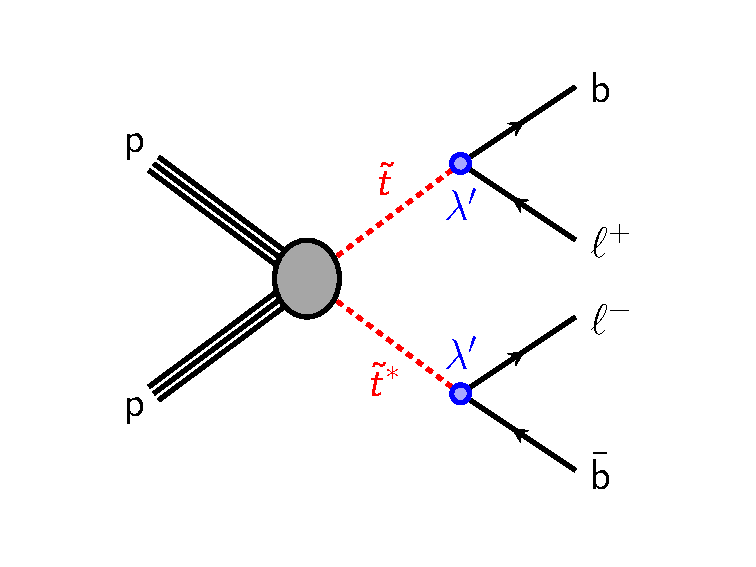
\includegraphics[width=0.60\textwidth]{figs/blstop/b_minus_l_stop_stop.pdf}
  \caption{Simplified model of pair production of stop quarks, with decay to a
    charged lepton and $b$-quark.
  }
  \label{fig:blstop_diagram}
\end{figure}

%% -----------------------------------------------------------------------------
\section{Object selection}
\label{sec:object_selection}

Events are required to have at least two light leptons (electrons or muons)
with opposite charge, and two $b$-tagged jets.
The object selection is performed in multiple steps. First, lepton and jet
objects are reconstructed using detector signatures as described in
Sections~\ref{sec:elctrons},~\ref{sec:muons},~and~\ref{sec:jets}.
Baseline requirements are applied to remove poorly reconstructed objects.
Also, all baseline objects are required to have $\ET(\pt) \geq 40 \GeV$ since the
stop signatures of interest tend to produce high momentum decay products.

%% - - - - - - - - - - - - - - - - - - - - - - - - - - - - - - - - - - - - - - -
%% baseline electrons
%% - - - - - - - - - - - - - - - - - - - - - - - - - - - - - - - - - - - - - - -
Baseline electrons must satisfy the \texttt{Medium++} identification
requirement and have $|\eta| \leq 2.47$.
A requirement of $\DZEROSIG \leq 3$ and $\ZZEROSINTHETA \leq 0.4$ mm
is placed on the impact parameter to reject electrons coming from secondary
vertices.
The baseline electron requirements are outlined in
Table~\ref{tab:baseline_el_def}.

\begin{table}[ht]
\caption{Baseline electron requirements.}
\label{tab:baseline_el_def}
\centering{
  \begin{tabular}{cc}
    \toprule
    Quality        & \texttt{Medium++} \\
    $p_T$          & $\geq 40 \GeV$    \\
    $|\eta|$       & $\leq 2.47$       \\
    \DZEROSIG      & $\leq 3$          \\
    \ZZEROSINTHETA & $\leq 0.4$ mm     \\
    \bottomrule
  \end{tabular}
}
\end{table}

%% - - - - - - - - - - - - - - - - - - - - - - - - - - - - - - - - - - - - - - -
%% baseline muons
%% - - - - - - - - - - - - - - - - - - - - - - - - - - - - - - - - - - - - - - -
Baseline muons are selected from the \texttt{STACO} muon collection, and
required to pass the \texttt{Loose} identification requirement. The baseline
muons must also have $|\eta| \leq 2.5$ 
Impact parameter requirements of $\DZEROSIG \leq 3$ and
$\ZZEROSINTHETA \leq 1$ mm are applied to reduce the contamination of muons
from secondary vertices and cosmic rays.
Additional requirements are applied on the number of hits in the ID to ensure
high quality tracks.
These  hit requirements include at least one hit on track in both the B layer
and the Pixel detector.
The ID track must also have at least 5 hits in the SCT, at most 2 missing 
hits-on-track (holes) in both the Pixel detector and the SCT. 
If the muon has $|\eta| \leq 1.9$, there must additionally be at least 6 TRT
hits, of which no more than 90\% are outliers.
Otherwise, no requirement is placed on the number of TRT hits.
The baseline muon requirements are outlined in Table~\ref{tab:baseline_mu_def}.

\begin{table}[ht]
  \caption{Baseline muon requirements.}
  \label{tab:baseline_mu_def}
  \centering{
    \begin{tabular}{cc}
      \toprule
      Quality              & \texttt{Loose} \\
      $p_T$                & $\geq 40 \GeV$ \\
      $|\eta|$             & $\leq 2.5$     \\
      Number B layer hits  & $\geq 1$       \\
      Number Pixel hits    & $\geq 1$       \\
      Number SCT hits      & $\geq 5$       \\
      Number Silicon holes & $\leq 2$       \\
      TRT hits             & See text       \\
      \DZEROSIG            & $\leq 3$       \\
      \ZZEROSINTHETA       & $\leq 1$ mm    \\
      \bottomrule
    \end{tabular}
  }
\end{table}

%% - - - - - - - - - - - - - - - - - - - - - - - - - - - - - - - - - - - - - - -
%% baseline jets
%% - - - - - - - - - - - - - - - - - - - - - - - - - - - - - - - - - - - - - - -
Baseline jets are selected from the AntiKt4LCTopo jet collection, and required
to have $|\eta| \leq 4.9$.
The baseline jet requirements are outlined in Table~\ref{tab:baseline_jet_def}.

\begin{table}[ht]
    \caption{Baseline jet requirements.}
    \label{tab:baseline_jet_def}
  \centering{
    \begin{tabular}{cc}
      \toprule
      $p_T$    & $\geq 40 \GeV$ \\
      $|\eta|$ & $\leq 4.9$     \\
      \bottomrule
    \end{tabular}
  }
\end{table}

%% - - - - - - - - - - - - - - - - - - - - - - - - - - - - - - - - - - - - - - -
%% overlap removal
%% - - - - - - - - - - - - - - - - - - - - - - - - - - - - - - - - - - - - - - -
After selecting baseline leptons and jets, overlap between baseline objects are
is removed to prevent a single detector signature from being included in
multiple particle collections. 

\begin{enumerate}
  \item $\Delta R(e,e) \le 0.05$: If two baseline electrons fall
    within a cone of $\Delta R(e,e) \le 0.05$, the electron with the
    lower \ET\ is removed from the event.
  \item $\Delta R(e,\mathrm{jet}) \le 0.20$: If a remaining electron and a jet
    are within a cone of $\Delta R(e,\mathrm{jet}) \le 0.20$, it is
    assumed that the electron is also reconstructed as a jet, and the
    jet is removed from the event.
  \item $\Delta R(\ell,\mathrm{jet}) \le 0.40$: If remaining lepton (electron
    or muon) and a remaining jet are within a cone of
    $\Delta R(\ell,\mathrm{jet}) \le 0.40$, the reconstructed lepton is assumed
    to be a constituent of the jet, and is removed from the event.
  \item $\Delta R(e,\mu) \le 0.01$: If a remaining electron and a remaining muon
    are within $\Delta R(e,\mu) \le 0.01$, both are removed from the event.
  \item $\Delta R(\mu,\mu) \le 0.05$: If two remaining muons are within
    $\Delta R(\mu,\mu) \le 0.05$, both are removed from the event.
\end{enumerate}

To reject leptons coming from low mass resonances, the invariant mass of any
remaining same-flavor lepton pairs with opposite charge is computed.
If the invariant mass of any of these pairs is less than 12~\GeV, both leptons
are removed from the event.

%% - - - - - - - - - - - - - - - - - - - - - - - - - - - - - - - - - - - - - - -
%% signal object definitions
%% - - - - - - - - - - - - - - - - - - - - - - - - - - - - - - - - - - - - - - -
Additional requirements are placed on the leptons and jets after overlap
removal to select the final ``signal'' objects.
The scalar sum of the momentum of all tracks with $\pt \geq 400 \GeV$
within a cone of $\Delta R \leq 0.30$ of a lepton ($\pt^\mathrm{cone30}$) is
used to determine if the lepton is isolated.
Both electrons and muons require
$\nicefrac{\pT^{\mathrm{cone30}}}{\min(p_T, 60 \GeV)} \leq 0.1$ in order
to be declared signa leptons.
Jets must pass a tighter cut of $|\eta| \leq 2.4$, and be tagged as a $b$-jet
using the 80\% working point of $\mathrm{MV1} \geq 0.3511$

Events are required to have at least two signal leptons and two $b$-tagged jets.
If more are found, the event is kept, but only the two signal leptons and two
$b$-tagged jets with the highest \pt\ are selected.
Furthermore, the two highest \pt\ leptons are required to have opposite charge.

%% - - - - - - - - - - - - - - - - - - - - - - - - - - - - - - - - - - - - - - -
%% pairing
%% - - - - - - - - - - - - - - - - - - - - - - - - - - - - - - - - - - - - - - -
To construct the mass of each of the $b\ell$ pairs, the leptons and $b$-tagged
jets must be paired.
It is possible to exploit the fact that in the target signal model, each
$b\ell$ pair comes from a resonant decay of a stop particle, and should
reconstruct the same invariant mass.
Therefore, the pairing which minimizes the difference in mass between the two
$b\ell$ pairs is selected as follows.

The two signal leptons and two $b$-jets are labeled $\ell_0$, $\ell_1$, $b_0$,
and $b_1$.

% Define some colors for this section to make changing colors easier
\colorlet{pairing_l_0}{green!50!white}
\colorlet{pairing_l_1}{green!20!white}
\colorlet{pairing_b_0}{red!50!white}
\colorlet{pairing_b_1}{red!20!white}
%
\begin{center}
  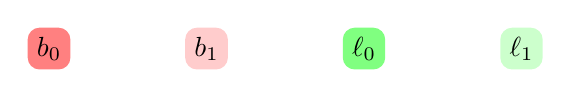
\begin{tikzpicture}
    \node[rectangle, rounded corners=1ex, fill=pairing_b_0, text=black] (b0) at (-3,0) {$b_0$};
    \node[rectangle, rounded corners=1ex, fill=pairing_b_1, text=black] (b1) at (-1,0) {$b_1$};
    \node[rectangle, rounded corners=1ex, fill=pairing_l_0, text=black] (l0) at (+1,0) {$\ell_0$};
    \node[rectangle, rounded corners=1ex, fill=pairing_l_1, text=black] (l1) at (+3,0) {$\ell_1$};
  \end{tikzpicture}
\end{center}
%
There are two possible choices of pairings for these four objects.
%
\begin{center}
  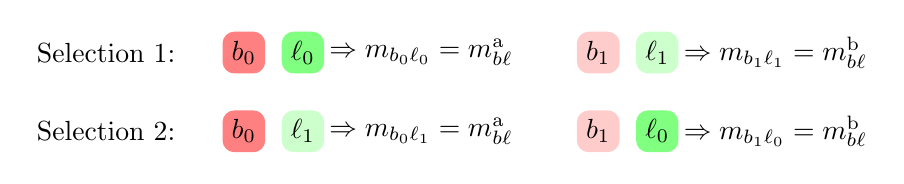
\begin{tikzpicture}
    \node[rectangle, text=black] (sel1) at (-5.0,+0.5) {Selection 1:};
    \node[rectangle, text=black] (sel2) at (-5.0,-0.5) {Selection 2:};

    \node[rectangle, rounded corners=1ex, fill=pairing_b_0, text=black] (b1) at (-3.25,+0.5) {$b_0$};
    \node[rectangle, rounded corners=1ex, fill=pairing_l_0, text=black] (l0) at (-2.50,+0.5) {$\ell_0$};
    \node[rectangle, rounded corners=1ex, fill=pairing_b_1, text=black] (b1) at (+1.25,+0.5) {$b_1$};
    \node[rectangle, rounded corners=1ex, fill=pairing_l_1, text=black] (l1) at (+2.00,+0.5) {$\ell_1$};
    \node[rectangle, text=black] (m00) at (-1.0,+0.5) {$\Rightarrow m_{b_0\ell_0} = m_{b\ell}^\mathrm{a}$};
    \node[rectangle, text=black] (m11) at (+3.5,+0.5) {$\Rightarrow m_{b_1\ell_1} = m_{b\ell}^\mathrm{b}$};

    \node[rectangle, rounded corners=1ex, fill=pairing_b_0, text=black] (b0) at (-3.25,-0.5) {$b_0$};
    \node[rectangle, rounded corners=1ex, fill=pairing_l_1, text=black] (l1) at (-2.50,-0.5) {$\ell_1$};
    \node[rectangle, rounded corners=1ex, fill=pairing_b_1, text=black] (b1) at (+1.25,-0.5) {$b_1$};
    \node[rectangle, rounded corners=1ex, fill=pairing_l_0, text=black] (l0) at (+2.00,-0.5) {$\ell_0$};
    \node[rectangle, text=black] (m01) at (-1.0,-0.5) {$\Rightarrow m_{b_0\ell_1} = m_{b\ell}^\mathrm{a} $};
    \node[rectangle, text=black] (m10) at (+3.5,-0.5) {$\Rightarrow m_{b_1\ell_0} = m_{b\ell}^\mathrm{b} $};
  \end{tikzpicture}
\end{center}

The masses of all pairings are calculated, and the pairing which gives the 
smallest difference in the mass $|\MBL^\mathrm{a} - \MBL^\mathrm{b}|$
is chosen.
The pairs are then ordered, and relabeled such that the higher mass pair has a
mass of $\MBL^{0}$, and the lower mass pair has a mass of $\MBL^{1}$.
This ensures $\MBL^{0} \geq \MBL^{1}$ by definition.

This heuristic correctly identifies at least one correct pairing of $b$-tagged
jets and leptons in roughly 65-90\% of events in the simulated signal samples
depending on the mass of the simulated stop. The efficiency, shown in
Figure~\ref{fig:pairing_eff}, improves once a cut is applied on the mass
asymmetry of the two $b\ell$ pairs as described in Section
\ref{sec:signal_regions}.

\begin{figure}[ht]
  \centering
  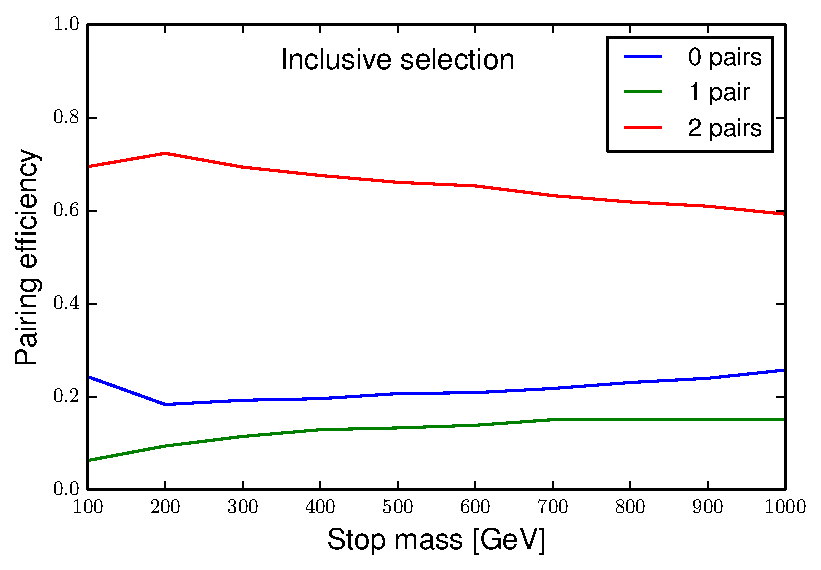
\includegraphics[width=0.60\textwidth]
    {figs/blstop/PairingEfficiencies/pairing_eff__inclusive.pdf}
  \caption{The efficiency of correctly pairing $b$-tagged jets and leptons
    using the pairing heuristic described in Section~\ref{sec:object_selection}
    for the different stop masses which are considered.
    The different lines show the fraction of events where zero, one, or two
    pairs are grouped correctly.
    The scenario where one pair is identified correctly corresponds to events
    where one pair is grouped correctly, but at least of of the $b$-tagged jets
    or one of the leptons is not matched to a stop parent.
    {\color{red} TODO remake this plot with 1.1~\TeV\ mass point. Add data
    points to plot}
  }
  \label{fig:pairing_eff}
\end{figure}

%% -----------------------------------------------------------------------------
\section{Event cleaning}
\label{sec:event_cleaning}

All sub-systems of the ATLAS detector are required to be operating acceptably
during data-taking. 
This data quality requirement is implemented using a good runs list (GRL)
provided by the Data Preparation group.\footnote{The GRL version
\texttt{data12\_8TeV.periodAllYear\_DetStatus-v61-pro14-02\_DQDefects-00-01-00\_PHYS\_StandardGRL\_All\_Good}
is used.}
By applying the GRL requirement, the total integrated luminosity is reduced
from 21.4~\ifb\ to 20.3~\ifb.
The uncertainty on the luminosity is $\pm 2.8$\%.
It is derived following the same methodology as that detailed
in Ref.~\cite{Lumi}.
The GRL requirement is applied to data events only; the MC simulation samples
are scaled to match the target luminosity.

% Several other detector errors can lead to an event being rejected.
In the event of a certain detector busy condition, the TTC may be restarted in
order to recover the detector without a full run-restart. In the lumi-block
after a TTC restart, it is possible for stored events to be incomplete.
For this reason, events stored immediately after a TTC restart are rejected.
Furthermore, events are rejected if either the LAr or tile calorimeter is
flagged as having an error.
During periods G-J several events are corrupt in a single channel of the tile
calorimeter, but not flagged as having a tile calorimeter error.
These events are also rejected using the \texttt{TileTripTool}.
During period B a hot spot developed in the tile calorimeter.
As this can negatively impact the jet calibration and the \met calculations,
events with a jet pointing toward this hot spot in the tile calorimeter are
rejected.

Jet cleaning is performed to flag jets which are formed from various sources
such as hardware problems, LHC beam conditions, or cosmic ray showers rather
than real energy deposits in the calorimeter.
If any of these bad jets remain after the overlap removal procedure, the event
is rejected.
Additionally, during periods E-H, a region of the LAr
calorimeter ($-0.1\le\eta\le1.5$ and $-0.9\le\phi\le-0.5$) malfunctioned
resulting in a hole in the sub-detector.
This resulted in energy not being collected from electrons and jets close to
this hole, and indirectly changing the \met\ measurement.
A correction is applied to jets to account for the energy loss in the hole,
however, if the correction is too large (greater than 0.05) and the \met\ is
close to the jet ($\Delta\phi(\met, \text{jet}) \le 0.3$), it is assumed the
\met\ is mismeasured, and the event is rejected.

In addition to the impact parameter requirement on muons discussed in
Section~\ref{sec:object_selection}, an additional requirement of
$|d_0| \leq 0.2$~mm is applied to muons passing the overlap removal to reject
muons from cosmic rays. Any event failing this selection requirement is
rejected.
In order to ensure muons are well measured, any event containing a muon after
overlap removal with $\sigma_{q/p}/|q/p| > 0.2$ is rejected.
These poorly measured muons can arise from the MS and ID reconstructing
different momenta for the same muon.

Each event is also required to have at least one primary vertex with at least
5 associated tracks.

An additional requirement is applied to MC simulation events to avoid double
counting backgrounds with heavy flavor quarks in the final state, the heavy
flavor overlap removal procedure, described in Section~\ref{sec:jet_matching},
is applied.

Events in data are taken from both the \texttt{egamma} and \texttt{muons} data
streams.
It is possible for the same event to exist in both streams, leading to the
possibility of double counting events.
To prevent this double counting of data events, the data stream is chosen based
on the flavor of the leading signal lepton in the event.
If the highest \pt\ event is an electron, the event is required to be found in
the \texttt{egamma} data stream.
Similarly, if the highest \pt\ lepton is a muon, the event is required to be
found in the \texttt{muons} data stream.
Events found in the wrong stream, are rejected.

%% -----------------------------------------------------------------------------
\section{Trigger selection}
\label{sec:trigger_selection}

A combination of four single-lepton triggers are used to select events.
The specific triggers used depend on the flavor channel of the event.
Di-electron(muon) events are required to pass at least one of the two single
electron (muon) triggers, while electron-muon events may pass any one of the
four triggers.
The specific triggers used for each flavor channel are outlined in
Table~\ref{tab:triggers}, and the trigger requirements are described in
Table~\ref{tab:trigger_defs}.

\begin{table}[ht]
  \caption{Trigger selection for each final state. If the event passes any of
    the triggers for the given final state, the event is accepted.
  }
  \label{tab:triggers}
  \centering{
    \begin{tabular}{cc}
      \toprule
      Final state & Trigger \\
      \midrule
      \multirow{2}{*}{$ee$bb}     &  \texttt{EF\_e24vhi\_medium1} \\
                                  &  \texttt{EF\_e60\_medium1}    \\
      \midrule
      $\mu\mu$bb                  &  \texttt{EF\_mu24i\_tight}    \\
      $\mu\mu$bb                  &  \texttt{EF\_mu36\_tight}     \\
      \midrule
      \multirow{3}{*}{$e\mu$bb}   &  \texttt{EF\_e24vhi\_medium1} \\
                                  &  \texttt{EF\_e60\_medium1}    \\
                                  &  \texttt{EF\_mu24i\_tight}    \\
                                  &  \texttt{EF\_mu36\_tight}     \\
      \bottomrule
    \end{tabular}
  }
\end{table}

\begin{table}[ht]
    \caption{Requirements for the triggers used in this analysis.  }
    \label{tab:trigger_defs}
  \centering{
    \begin{tabular}{c|cc}
      \toprule
      Trigger & \pt\ threshold & Other requirements \\
      \midrule
      \multirow{2}{*}{\texttt{EF\_e24vhi\_medium1}}
      & \multirow{2}{*}{$\pt^{e} \geq 24 \GeV$}
      & hadronic core isolation $\leq 1 \GeV$ \\
      & & $\nicefrac{\pt^\mathrm{cone20}}{\pt} < 0.1$ \\
      \texttt{EF\_e60\_medium1} & $\pt^{e} \geq 60 \GeV$ & -- \\
      \texttt{EF\_mu24i\_tight}
      & $\pt^{e} \geq 24 \GeV$
      & $\nicefrac{\pt^\mathrm{cone20}}{\pt} < 0.12$ \\
      \texttt{EF\_mu36\_tight}  & $\pt^{e} \geq 36 \GeV$ & -- \\
      \bottomrule
    \end{tabular}
  }
\end{table}

At least one of the reconstructed leptons is required to be within 
$\Delta R \leq 0.15$ of the detector signature found by the trigger.
The expected trigger efficiencies for simulated stop events are shown
for each trigger individually in Figure~\ref{fig:single_trigger_efficiency}.
The two muon triggers have roughly the same trigger efficiency, of about 93\% 
for $\mu\mu$ events and 75\% for $e\mu$ events, for all stop masses.
The two electron triggers, however, have dramatically different shapes, with
the \texttt{EF\_e24vhi\_medium1} trigger being highly efficient for $ee$ and
$e\mu$ events low mass from low mass stop, which decrease for higher
stop masses. 
The \texttt{EF\_e60\_medium1} trigger is not efficient for lower stop
masses, but quickly reaches approximately efficiencies above 95\% efficiency for
$ee$ and $e\mu$ events.

The dependence on the stop mass is a result of the \ET\ dependence of the
electron triggers.
The decay products of lighter stops tend to have lower momentum.
As a result, the electrons from the very light stops ($\leq 300~\GeV$) do not 
are more likely have \ET\ less than the threshold for the
\texttt{EF\_e60\_medium1} trigger.
Similarly, high-\HT\ electrons will deposit more energy into the calorimeter,
and some of this energy will reach the hadronic calorimeter.
As the electron \HT\ increases, the probability that the energy deposition into
the hadronic calorimeter is enough to fail hadronic core isolation requirement
of the \texttt{EF\_e24vhi\_medium1} trigger increases.
The \ET\ dependence of the two electron triggers, shown in
Figure~\ref{fig:electron_trigger_pt_dependence}, is consistent with the expected
dependence.

\begin{figure}[ht]
  \centering
  \subbottom[\texttt{EF\_e24vhi\_medium1}]{
    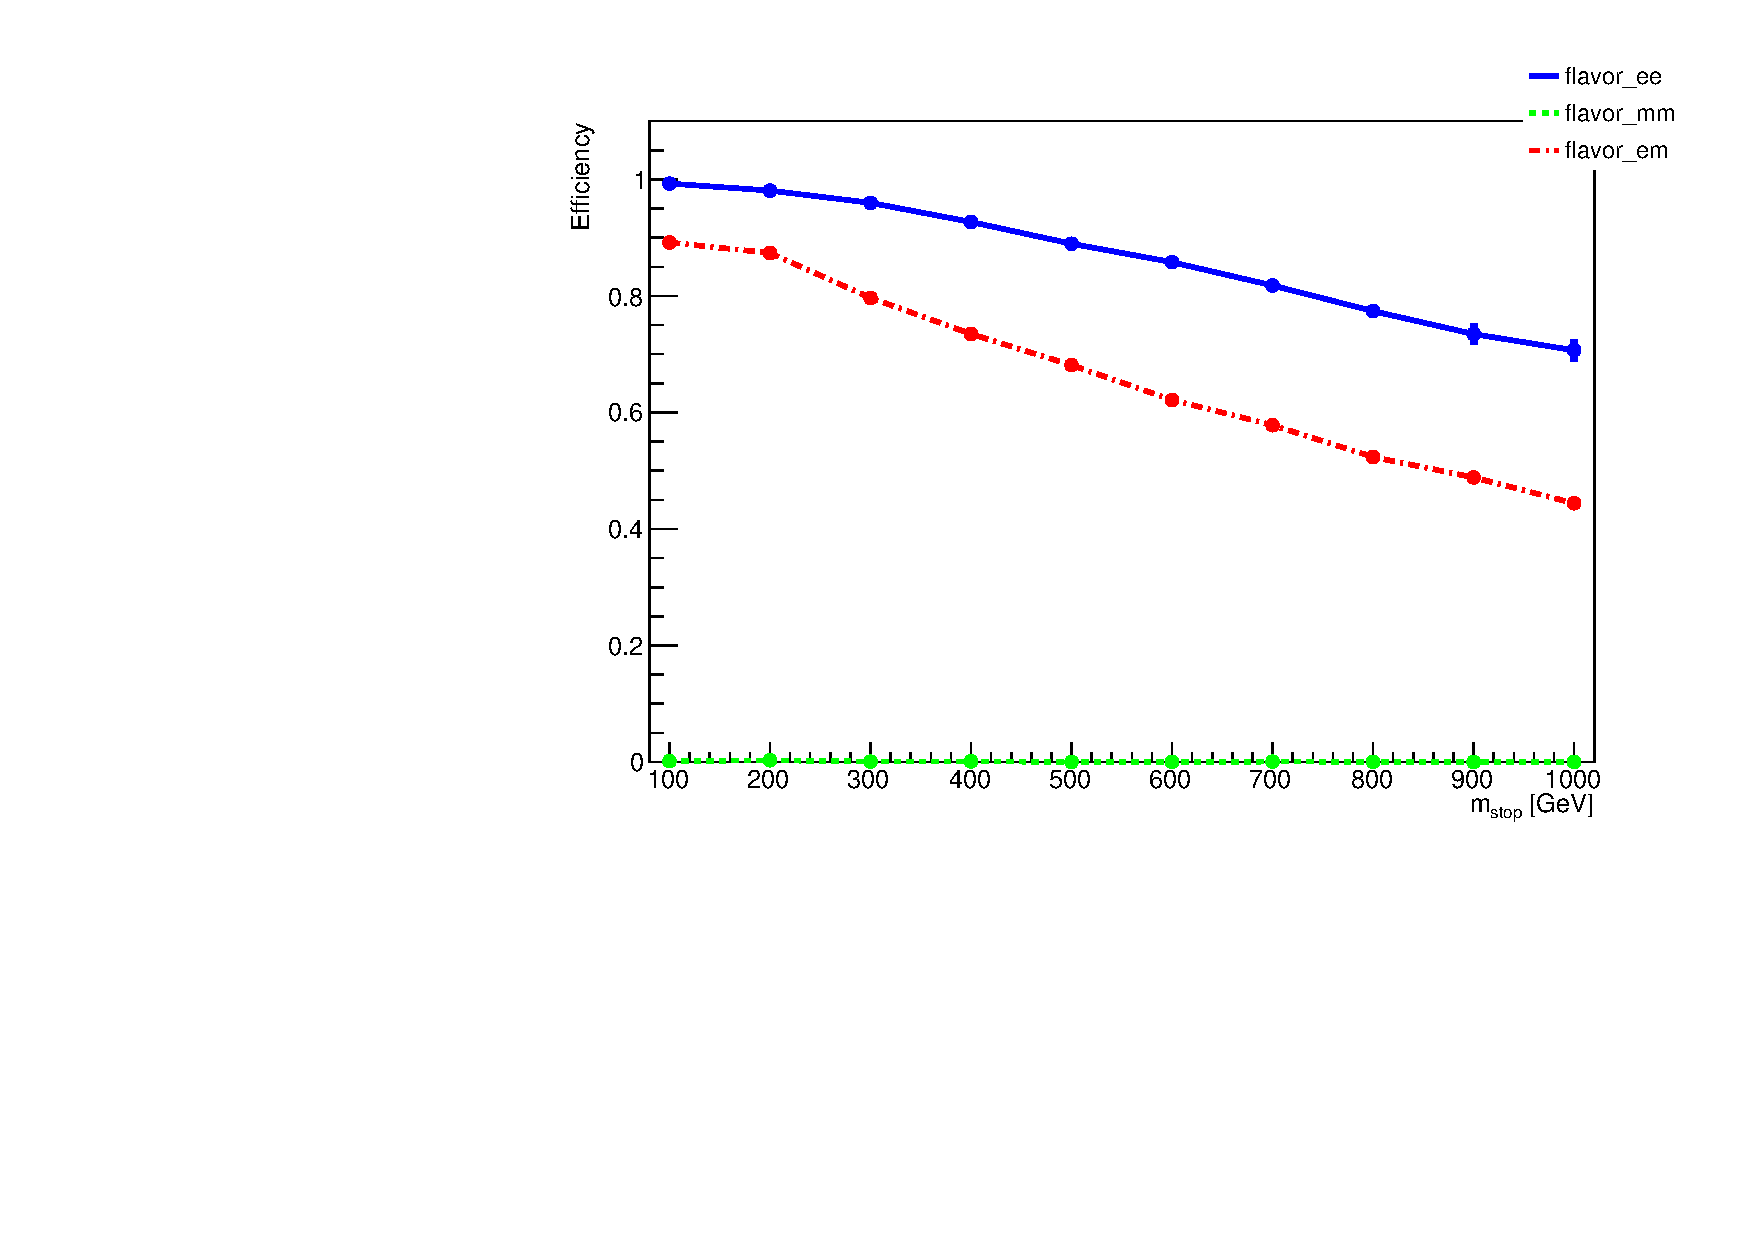
\includegraphics[width=0.48\textwidth]
      {figs/trigger/EF_e24vhi_medium1.pdf}
  }
  \subbottom[\texttt{EF\_e60\_medium1}]{
    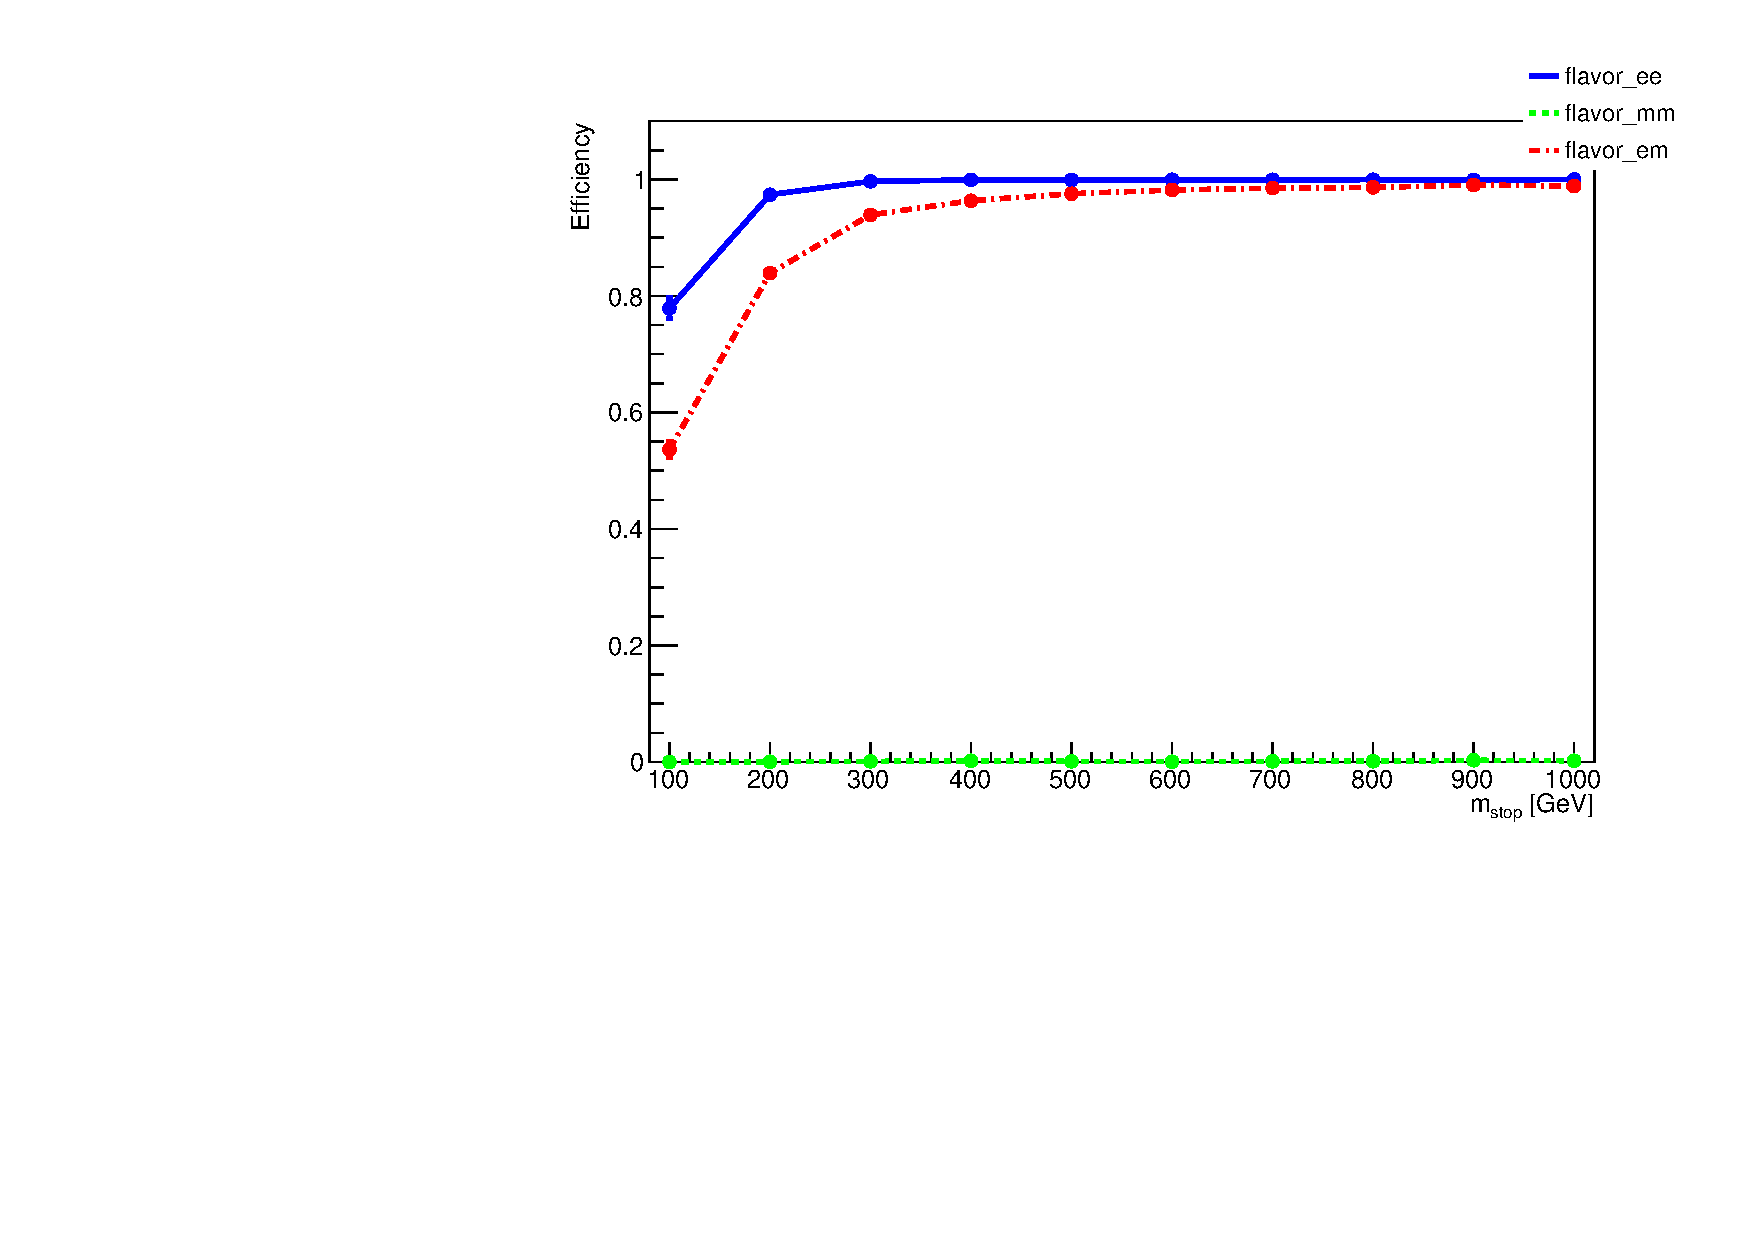
\includegraphics[width=0.48\textwidth]
      {figs/trigger/EF_e60_medium1.pdf}
  }
  \subbottom[\texttt{EF\_mu24i\_tight trigger}]{
    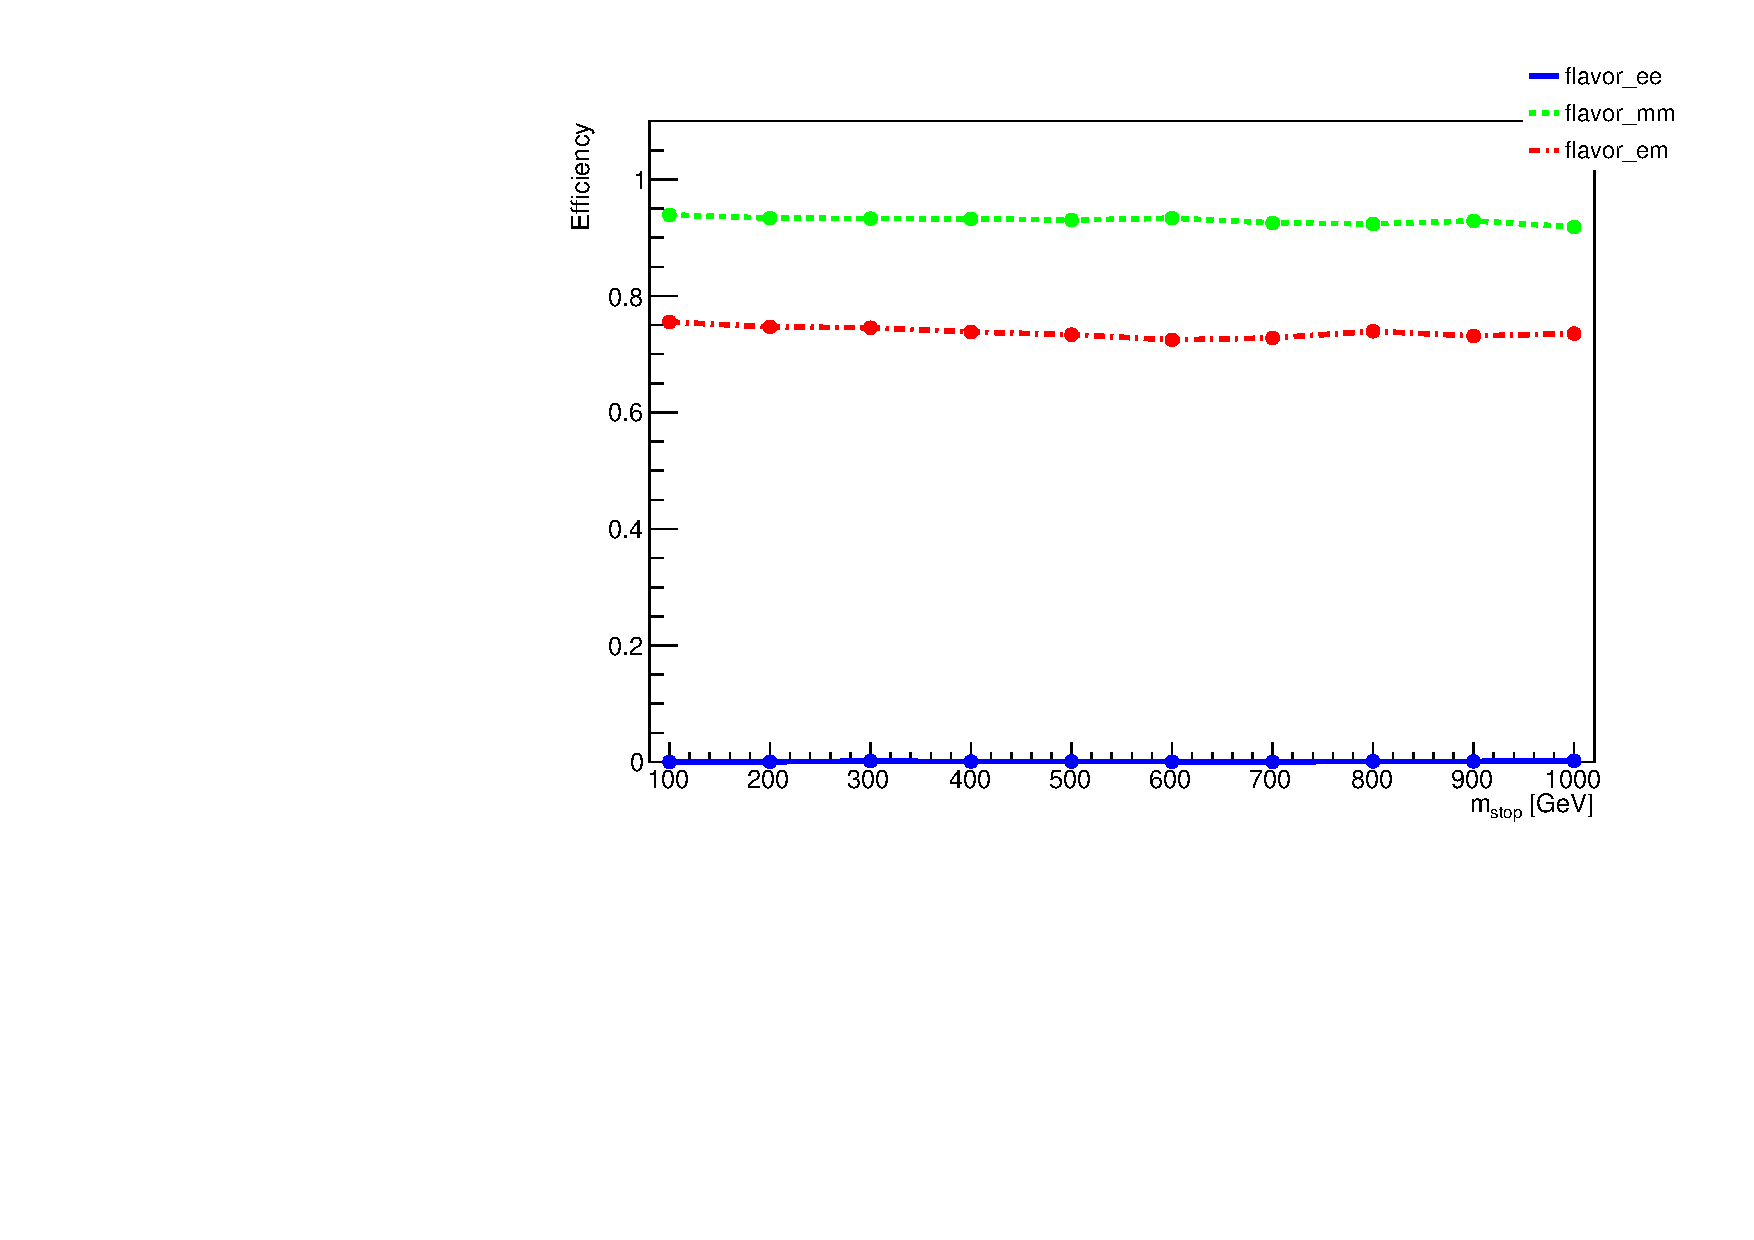
\includegraphics[width=0.48\textwidth]
      {figs/trigger/EF_mu24i_tight.pdf}
  }
  \subbottom[\texttt{EF\_mu36\_tight}]{
    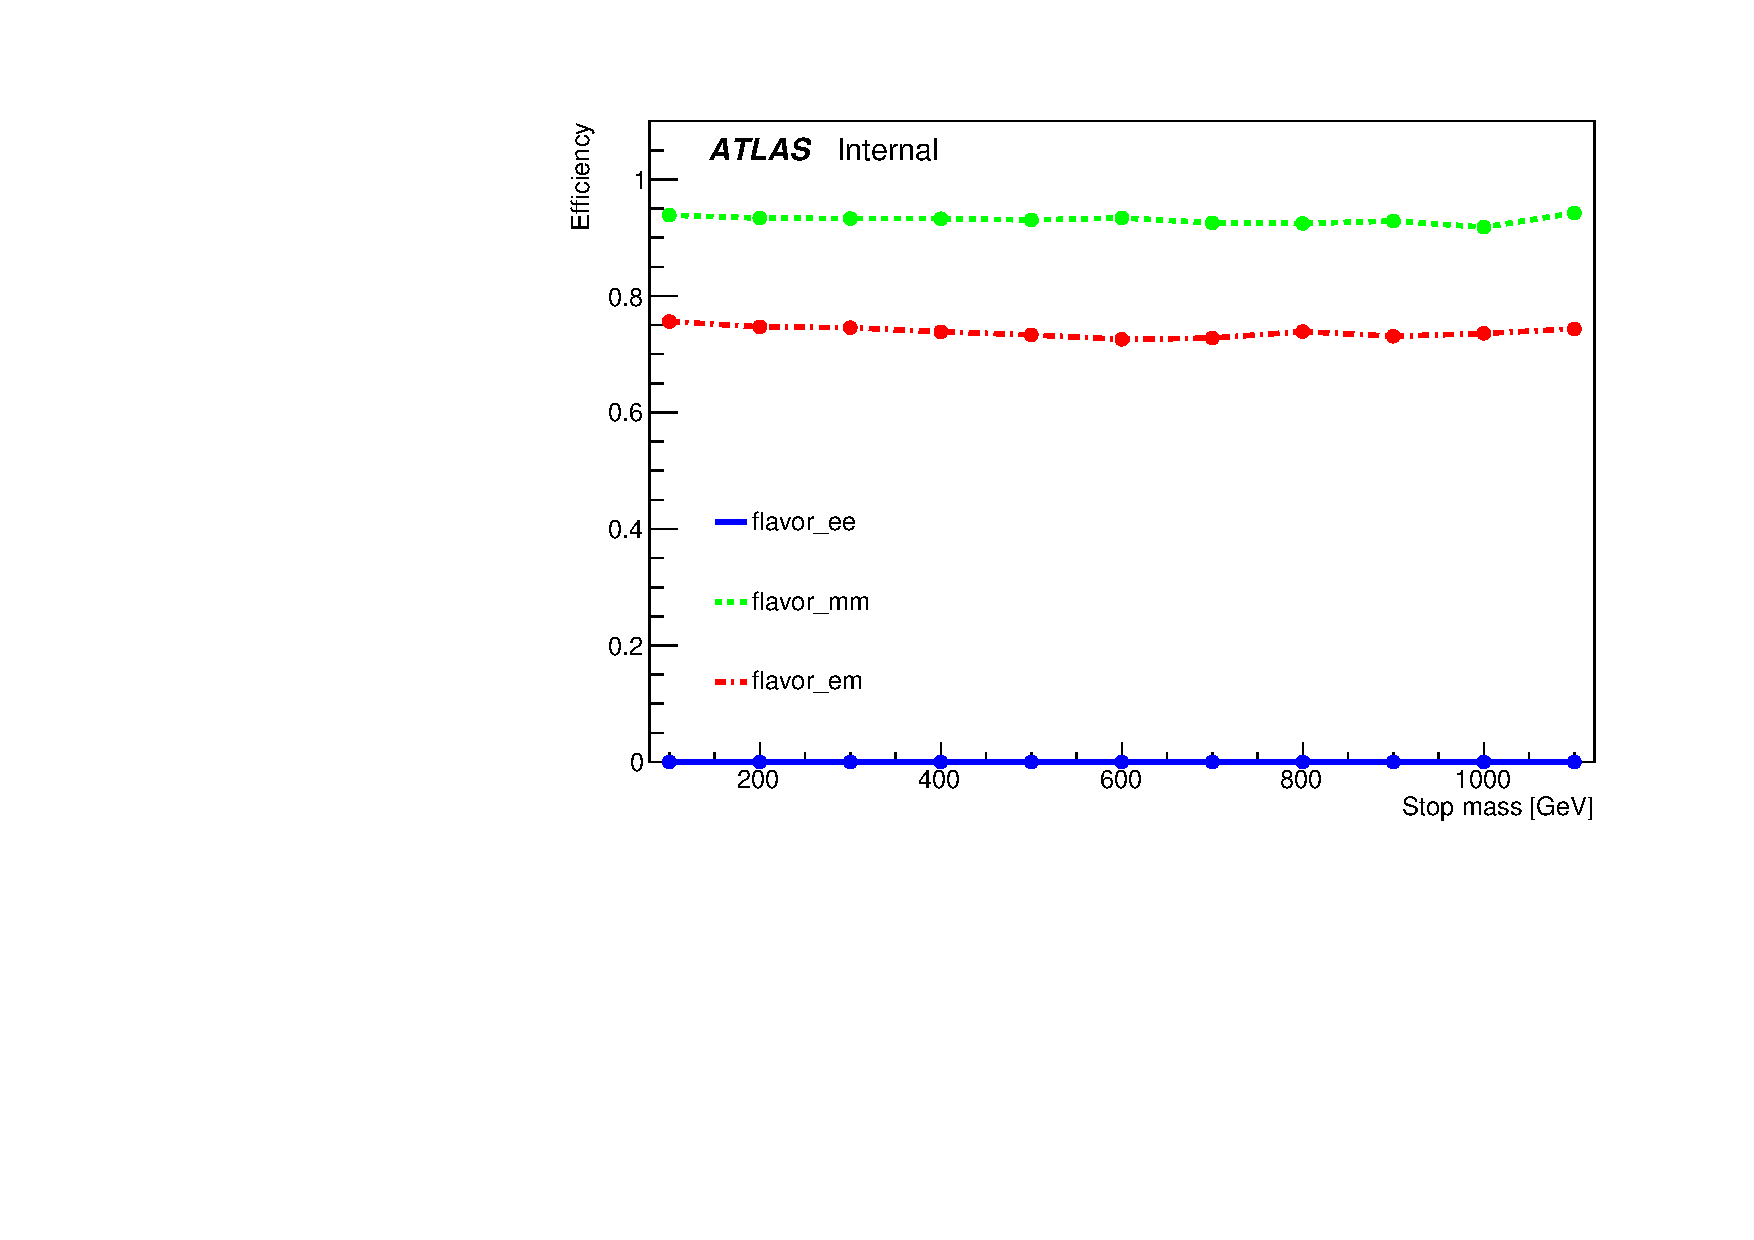
\includegraphics[width=0.48\textwidth]
      {figs/trigger/EF_mu36_tight.pdf}
  }
  \caption{Efficiency of simulated stop events passing each single lepton
    trigger broken down by flavor channel.
    The two single electron triggers have different shapes, which the 
    \texttt{EF\_e24vhi\_medium1} trigger being more efficient for low stop
    masses and the \texttt{EF\_e60\_medium1} trigger more efficient for
    higher stop masses.
    The two single muon triggers have roughly equal efficiency for all stop
    masses.
    Due to the trigger requirement, and the overlap removal procedure, $ee$
    events do not pass the single muon triggers, and $\mu\mu$ events do not
    pass the single electron triggers.
    {\color{red} TODO re-make these plots with overlap removal turned on and
    the 1100 \GeV\ point added}
  }
  \label{fig:single_trigger_efficiency}
\end{figure}

\begin{figure}[ht]
  \centering
  \subbottom[\texttt{EF\_e24vhi\_medium1}]{
    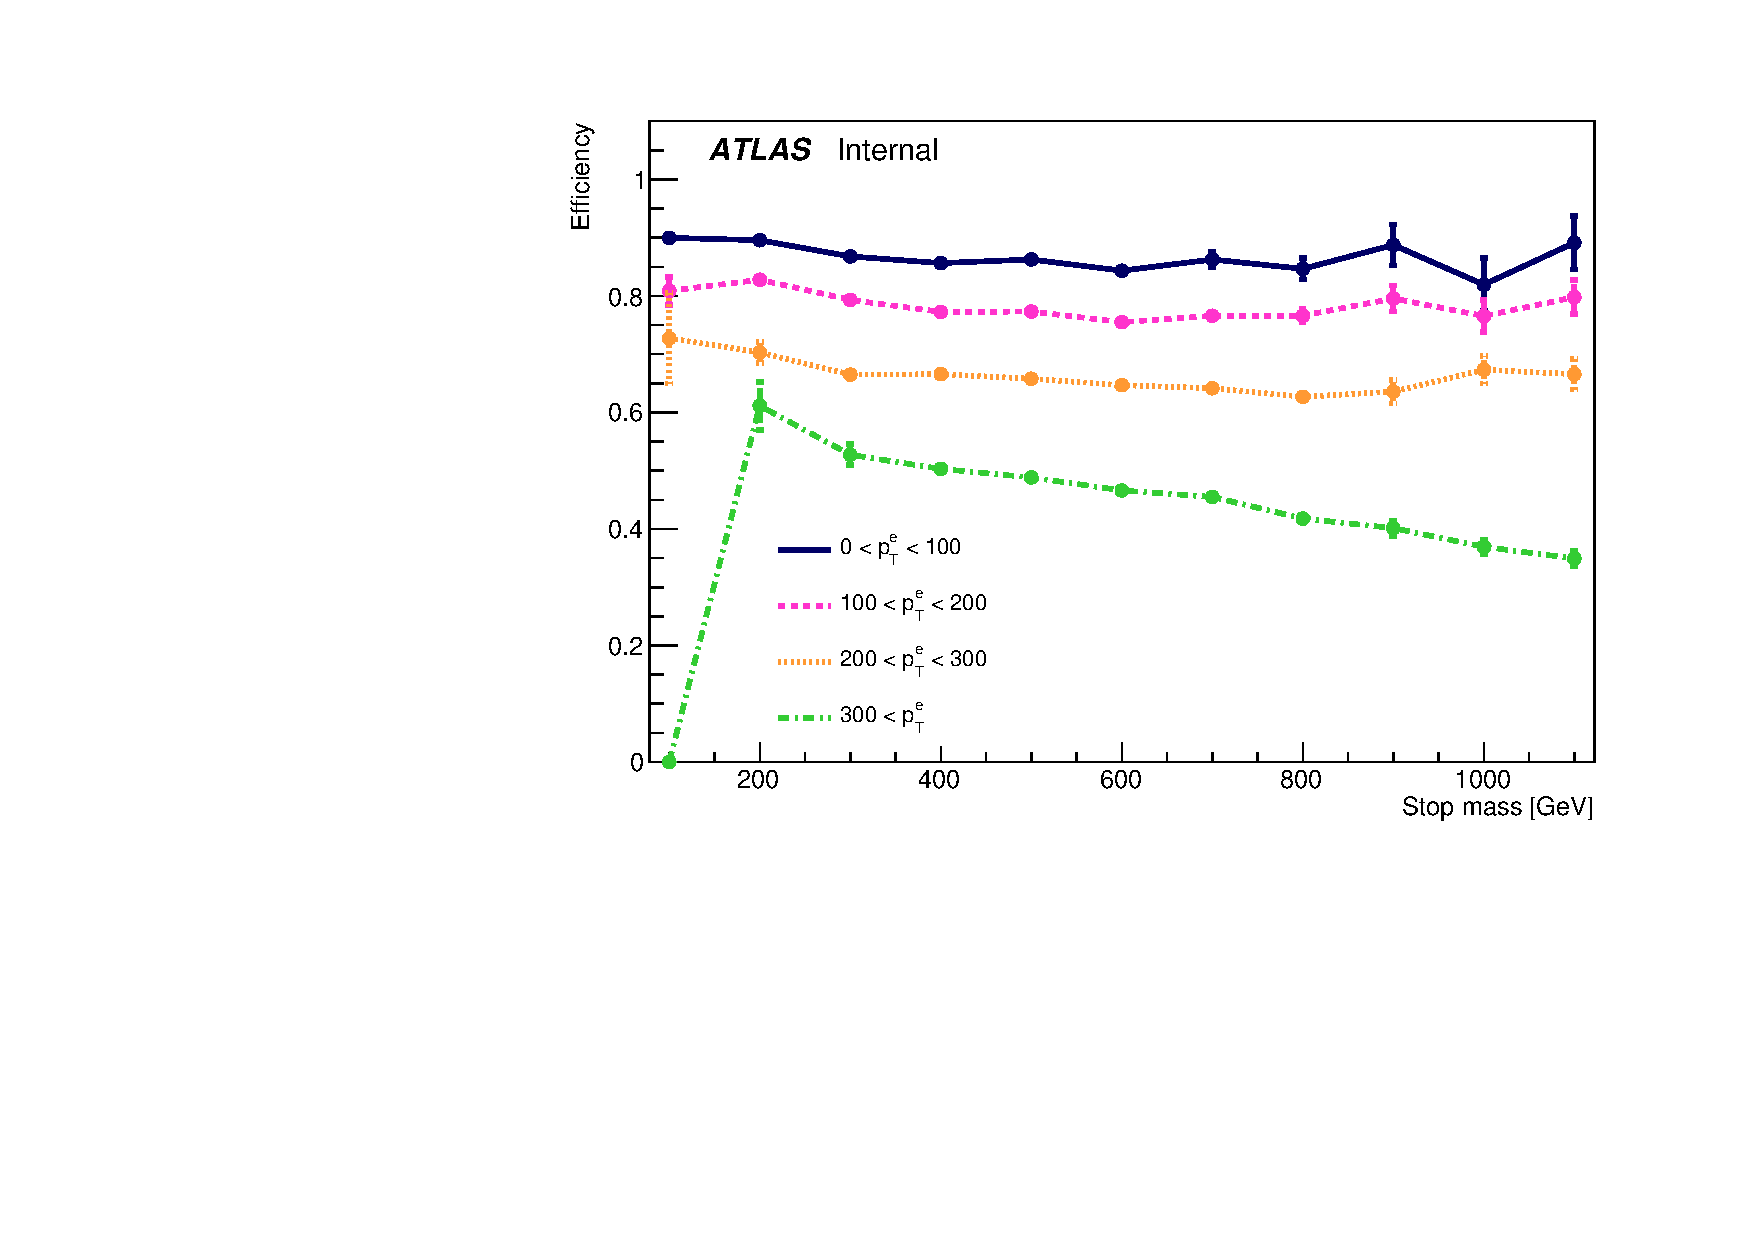
\includegraphics[width=0.48\textwidth, clip=true, trim=0 0 1cm 0]
      {figs/trigger/EF_e24vhi_medium1__el_pt.pdf}
  }
  \subbottom[\texttt{EF\_e60\_medium1}]{
    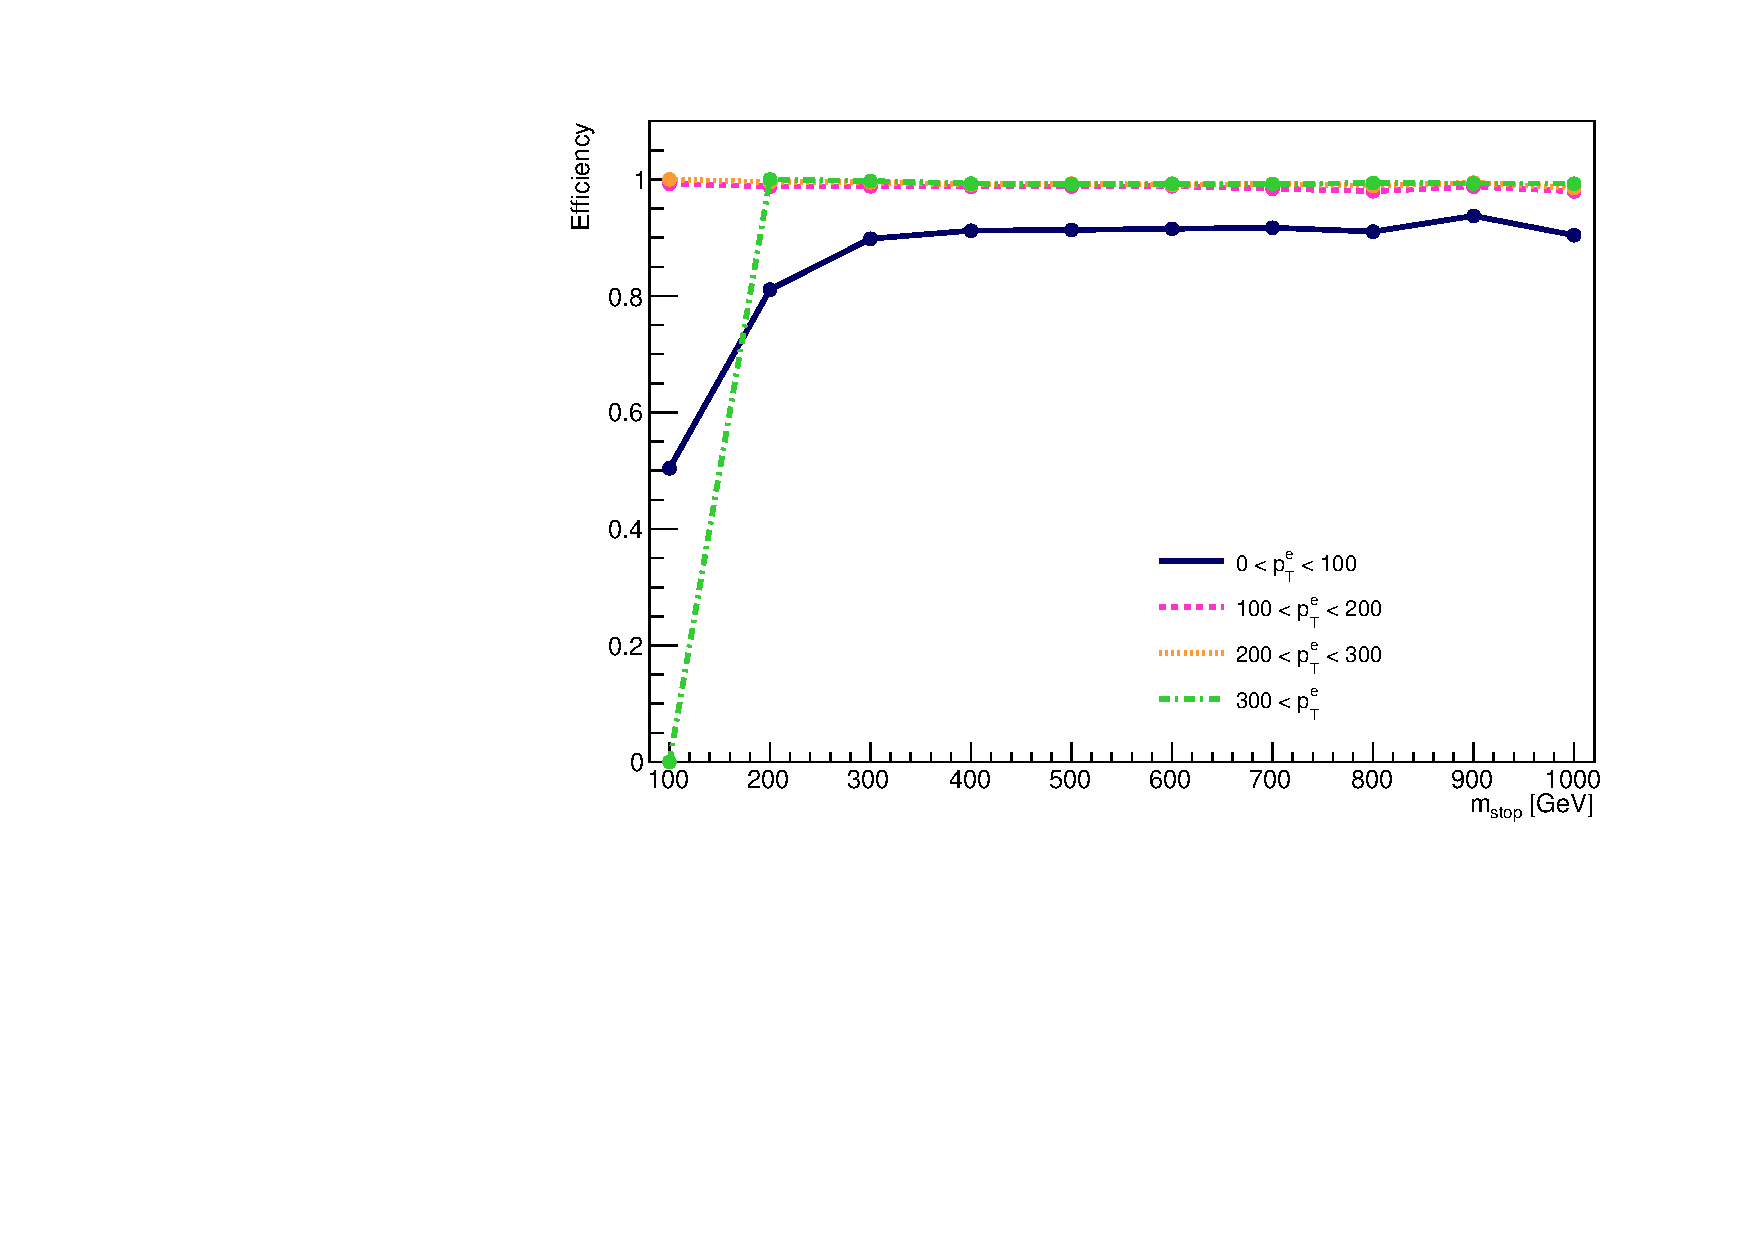
\includegraphics[width=0.48\textwidth, clip=true, trim=0 0 1cm 0]
      {figs/trigger/EF_e60_medium1__el_pt.pdf}
  }
  \caption{Efficiency of simulated stop events passing each of the single
    electron triggers for several ranges of electron \ET.
    Only $e\mu$ events are shown in order to show to isolate the effect of
    the electron \ET\ on the single electron trigger efficiency.
    These plots show the trigger efficiency dependence on the stop mass,
    observed in Figure~\ref{fig:single_trigger_efficiency} is due to a
    dependence on the electron \HT.
    The \texttt{EF\_e24vhi\_medium1} trigger has the high efficiency for low
    \HT\ electrons, while the \texttt{EF\_e60\_medium1} trigger is more
    efficient for high \HT\ electrons.
    {\color{red} TODO re-make these plots with overlap removal turned on and
    the 1100 \GeV\ point added}
  }
  \label{fig:electron_trigger_pt_dependence}
\end{figure}

The full trigger requirement is highly efficient for signal-like events; between
93\% and 98\% of simulated signal events pass the trigger selection depending
on the flavor channel as shown in Figure~\ref{fig:full_trigger_efficiency}.

\begin{figure}[ht]
  \centering
  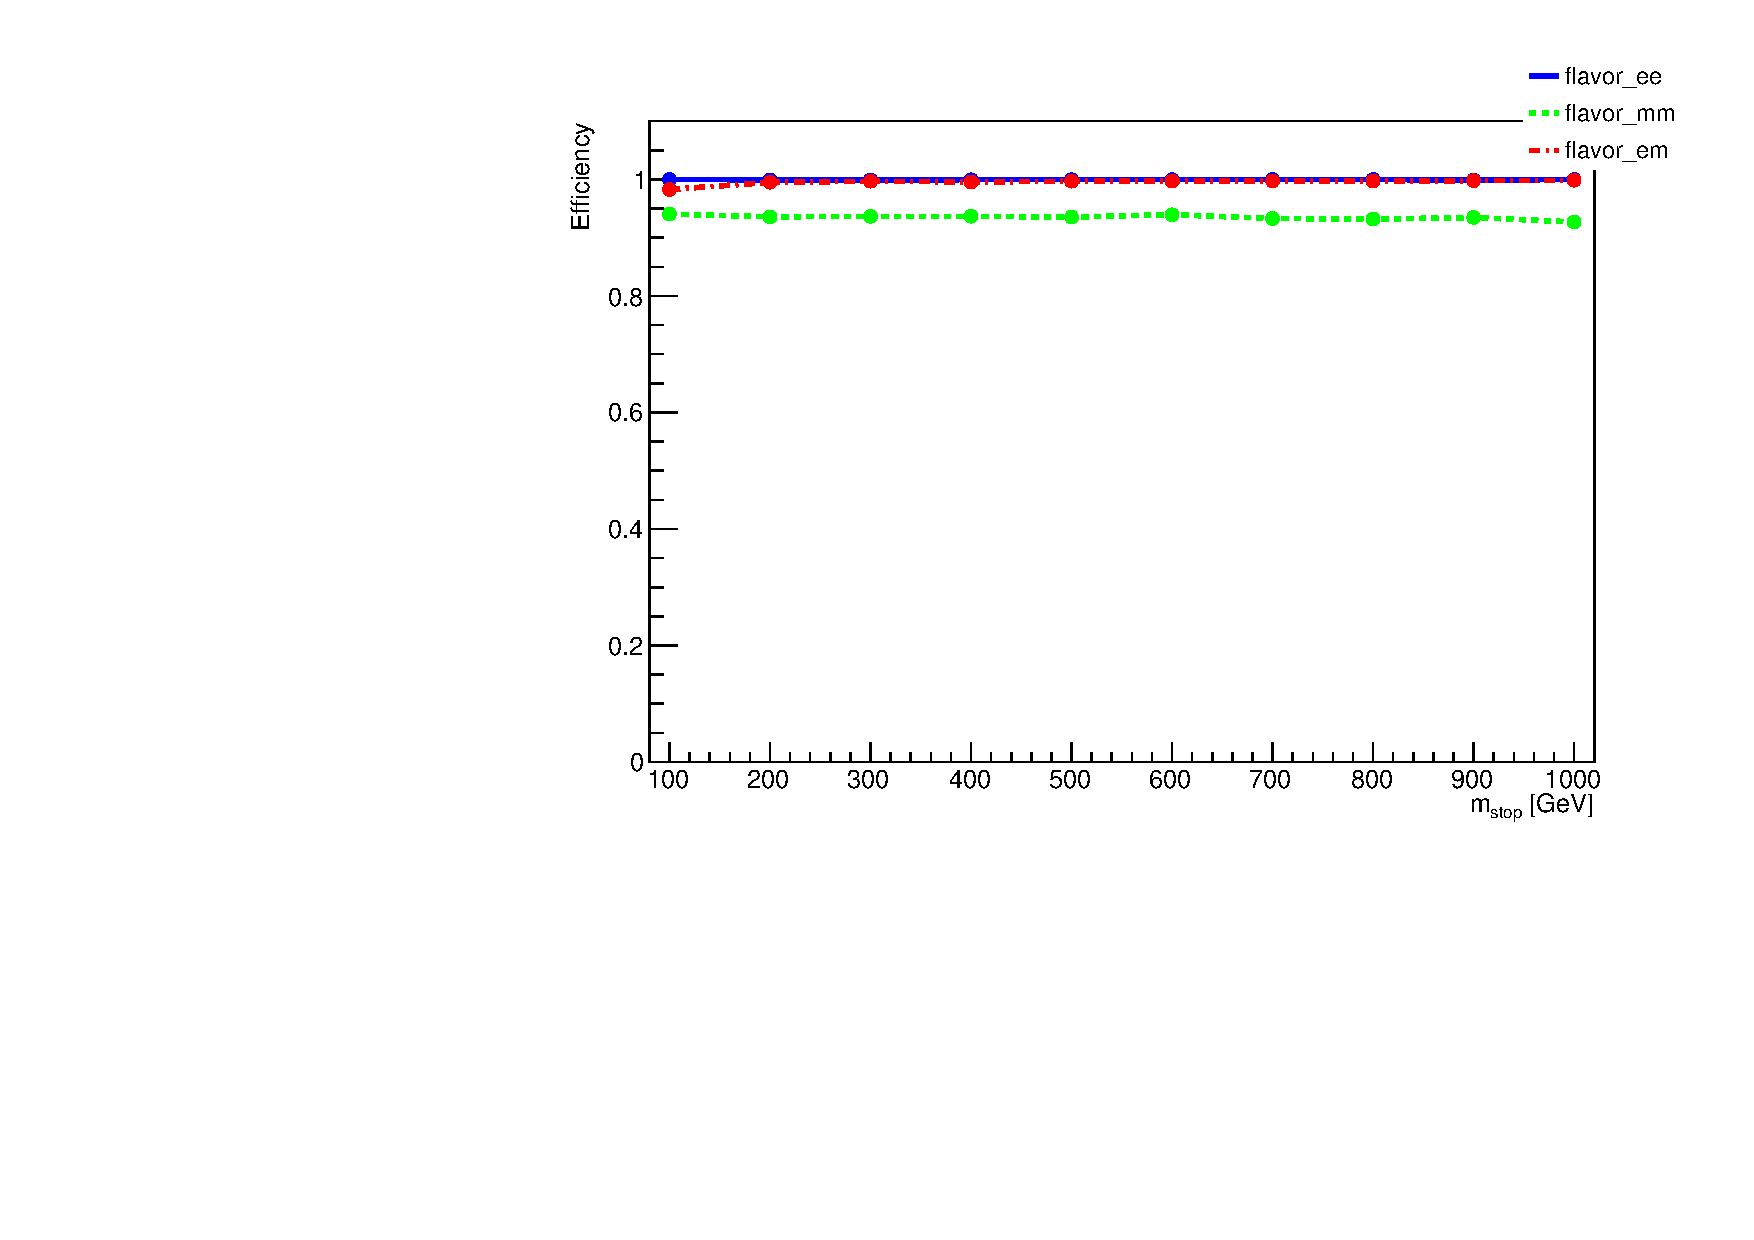
\includegraphics[width=0.60\textwidth]
    {figs/trigger/EF_e24vhi_medium1_OR_EF_e60_medium1_OR_EF_mu36_tight.pdf}
  \caption{Efficiency of simulated stop events passing the full trigger
    selection broken down by flavor channel.
    When the full trigger selection is considered, the trigger efficiency does
    not depend on the stop mass.
    {\color{red} TODO remake this plot using or of all four triggers (currently
      only shows the two electron triggers and the mu36 trigger). Also, include
      the 1100 GeV mass point.
    }
  }
  \label{fig:full_trigger_efficiency}
\end{figure}

%% -----------------------------------------------------------------------------
\section{Signal regions}
\label{sec:signal_regions}

This analysis targets a wide range of stop masses, which differ greatly in the
expected cross sections and the expected event kinematics.
For this reason, two overlapping signal regions (SRs) are defined to search for
an excess of signal-like events, which are inconsistent with the prediction from
the SM alone.
The two signal regions target the low stop mass and high stop mass regions
separately.

One of the major sources of SM background come from \ZGAMMAJETS.
To reduce this background, events where the two leptons have the same
flavor, and reconstruct an invariant mass consistent with the mass of the $Z$
boson ($|m_{\ell\ell} - m_{Z}| \leq 10 \GeV$) are rejected.

The scalar sum of the \pt\ of the two $b$-tagged jets and two leptons (\HT) 
effectively separates the signal processes from the major sources of
Standard Model background.
The stops of interest are extremely massive, so all the decay products tend to
have a large amount of energy, resulting in a high \HT.
SM processes, such as \TTBAR\ and \ZGAMMAJETS, do not have as large \HT.

For the signal model, the two $b\ell$ pairs making up the final state are the
decay products of the stop/anti-stop, and therefore have the same mass.
The mass asymmetry variable is defined as
\begin{equation}
  \MBLASYM = 
  \frac{\MBL^0-\MBL^1}{\MBL^0+\MBL^1}.
\end{equation}
Events from stop decays are expected to have low \MBLASYM\ as the mass
difference in the two pairs is expected to be small, while the masses of the
$b\ell$ pairs coming from SM processes are roughly uncorrelated, and there is
no preference for \MBLASYM.
The asymmetry is used rather than the simple difference in the masses so a
single cut value can be used for all stop masses which are considered.
Furthermore, events from SM background processes tend to have low \MBL\ for
both pairs.
The $\MBL^0$ variable can also provide additional discrimination power.
The expected \MLL, \HT, \MBLASYM\, and $\MBL^{0}$ distributions for SM
background processes and three signal models is shown in an inclusive region
after event cleaning and selecting two $b$-tagged jets and two leptons in
Figure~\ref{fig:no_data__no_k__inclusive_flavor_all__kinematic_dists}.

\begin{figure}
  \centering
  \subbottom[\MLL]{
    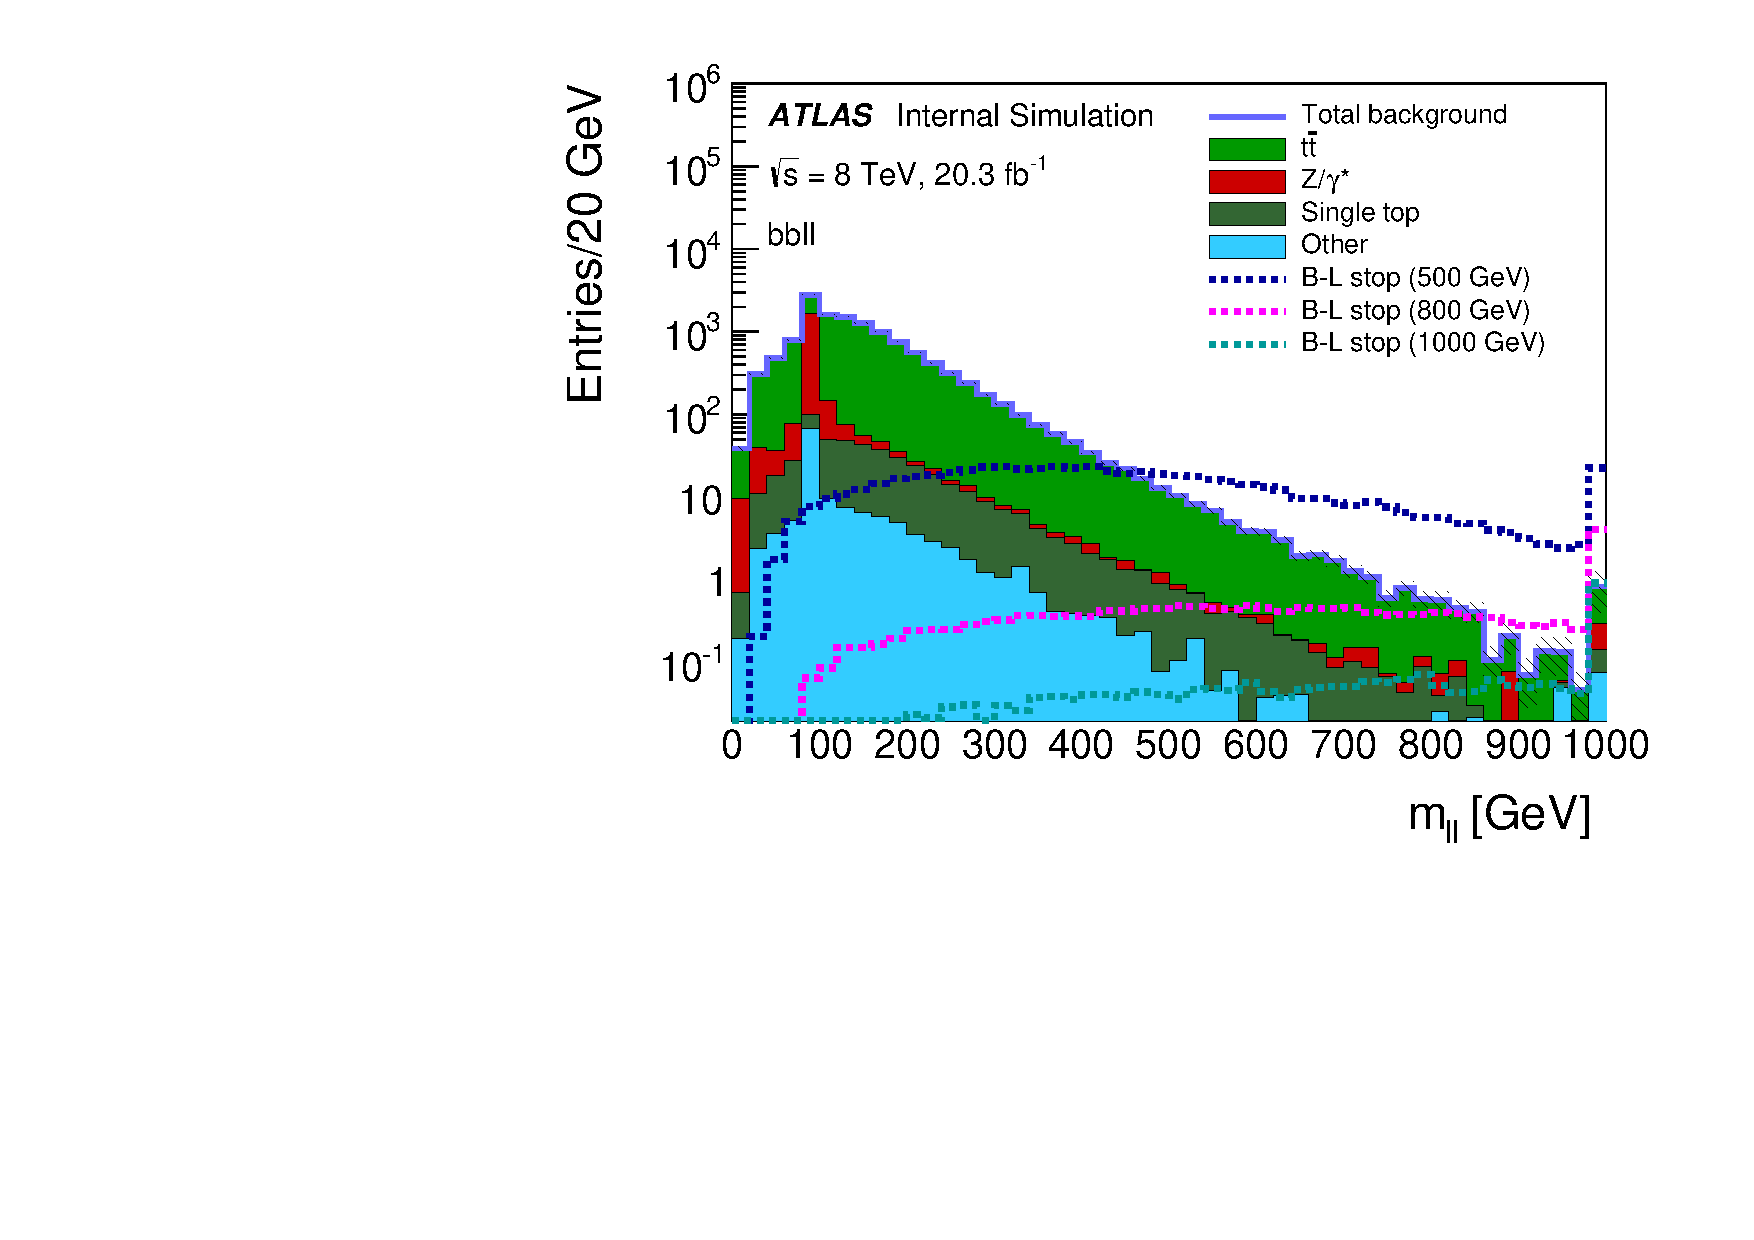
\includegraphics[width=0.48\textwidth, clip=true, trim=0 0 1cm 0]
    {figs/blstop/no_data__no_k_factor__dists/flavor_all__mll__BMINUSL_BL_PAIRING__log.pdf}
  }
  \subbottom[\HT]{
    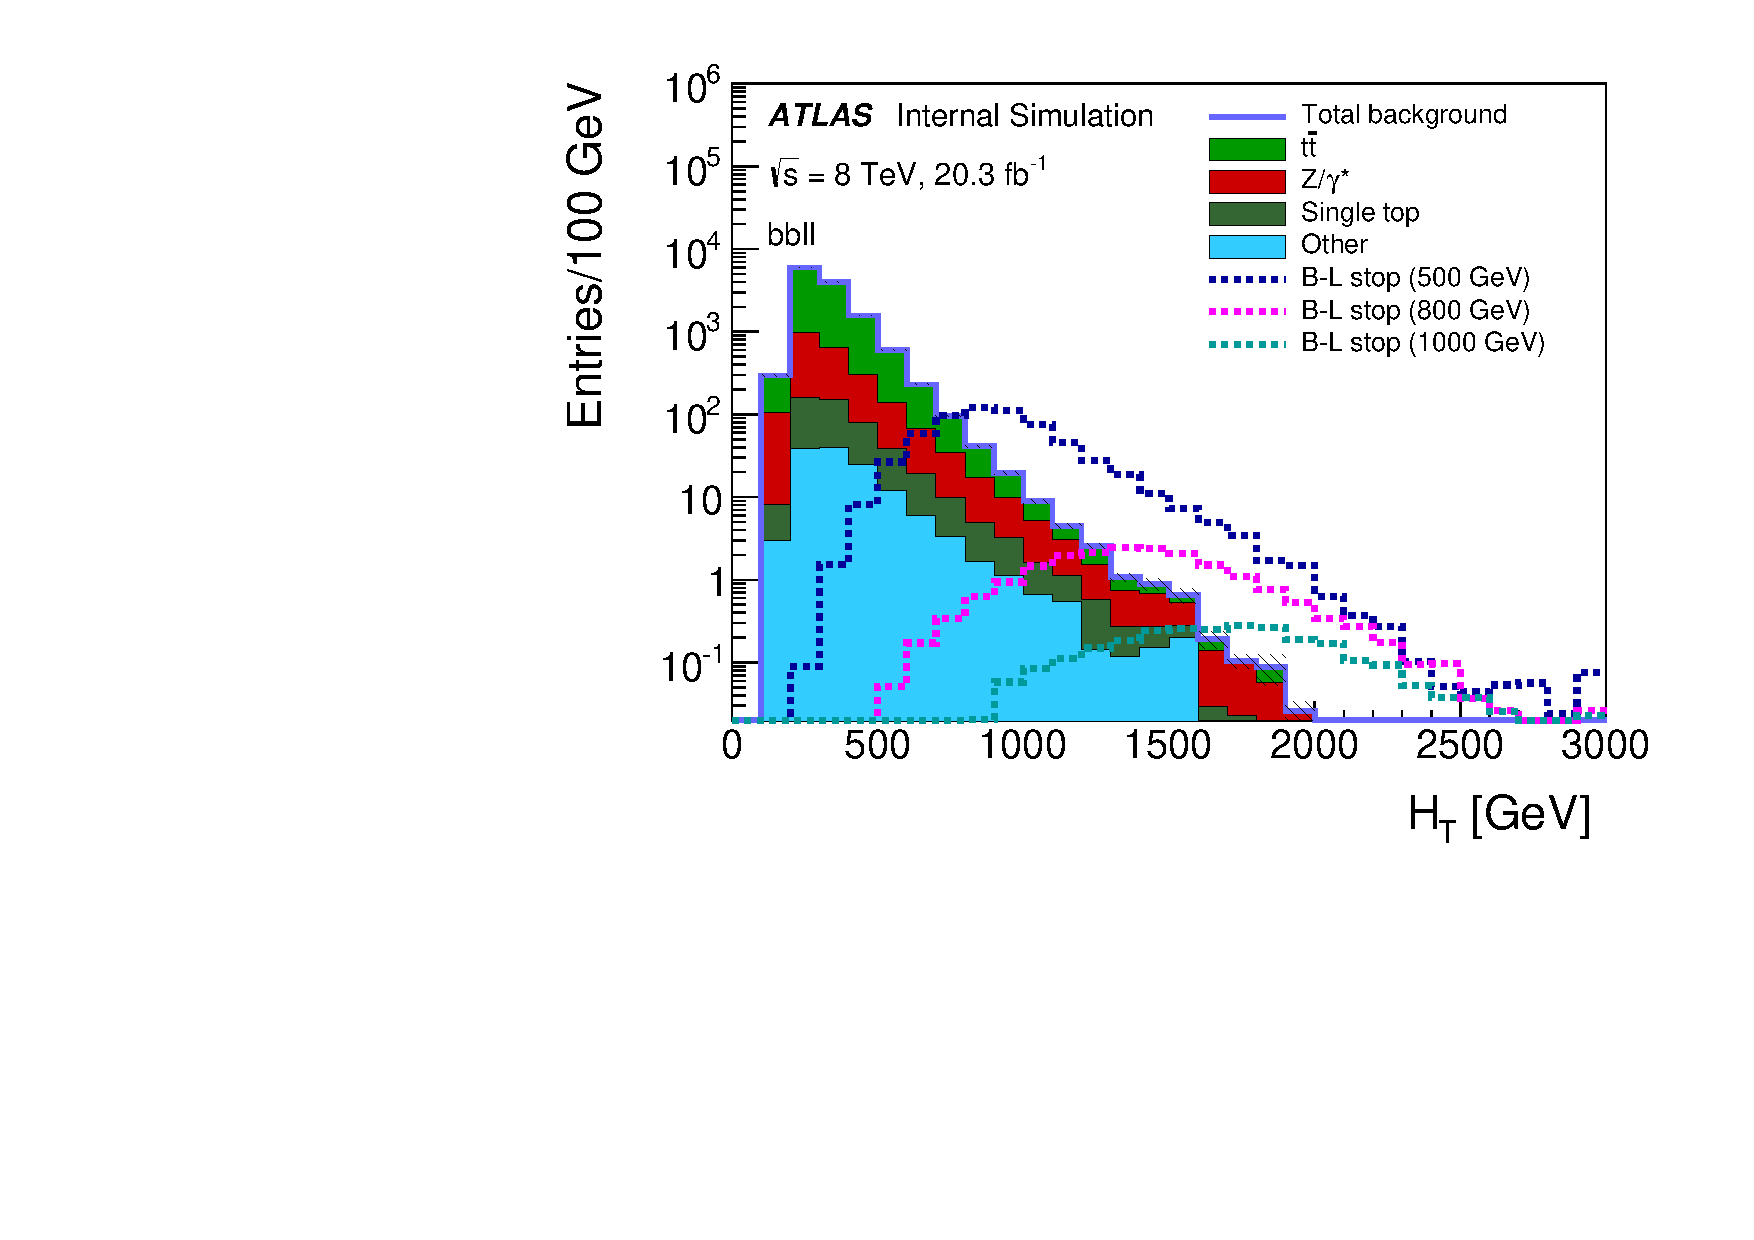
\includegraphics[width=0.48\textwidth, clip=true, trim=0 0 1cm 0]
    {figs/blstop/no_data__no_k_factor__dists/flavor_all__ht_signal__BMINUSL_BL_PAIRING__log.pdf}
  }
  \subbottom[\MBLASYM]{
    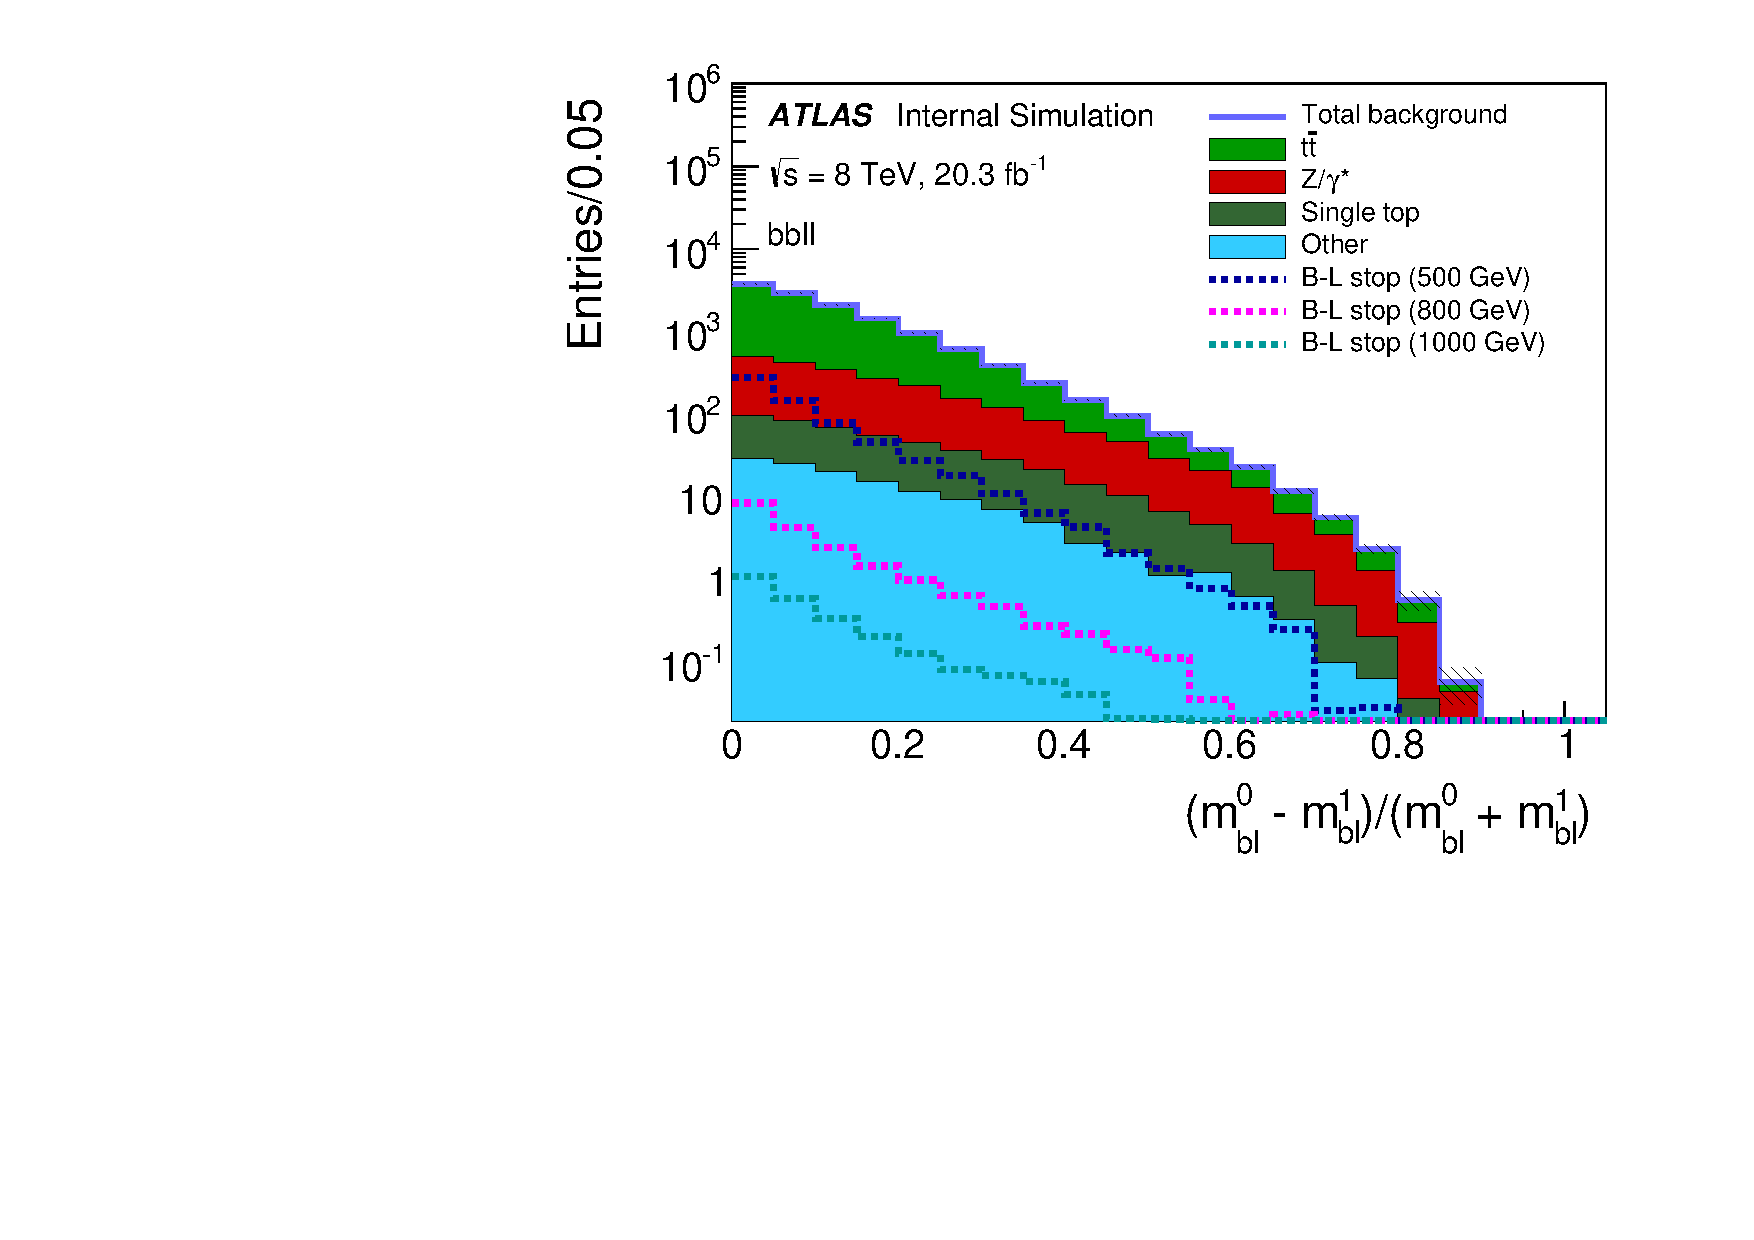
\includegraphics[width=0.48\textwidth, clip=true, trim=0 0 1cm 0]
    {figs/blstop/no_data__no_k_factor__dists/flavor_all__mbl_asym__BMINUSL_BL_PAIRING__log.pdf}
  }
  \subbottom[$\MBL^0$]{
    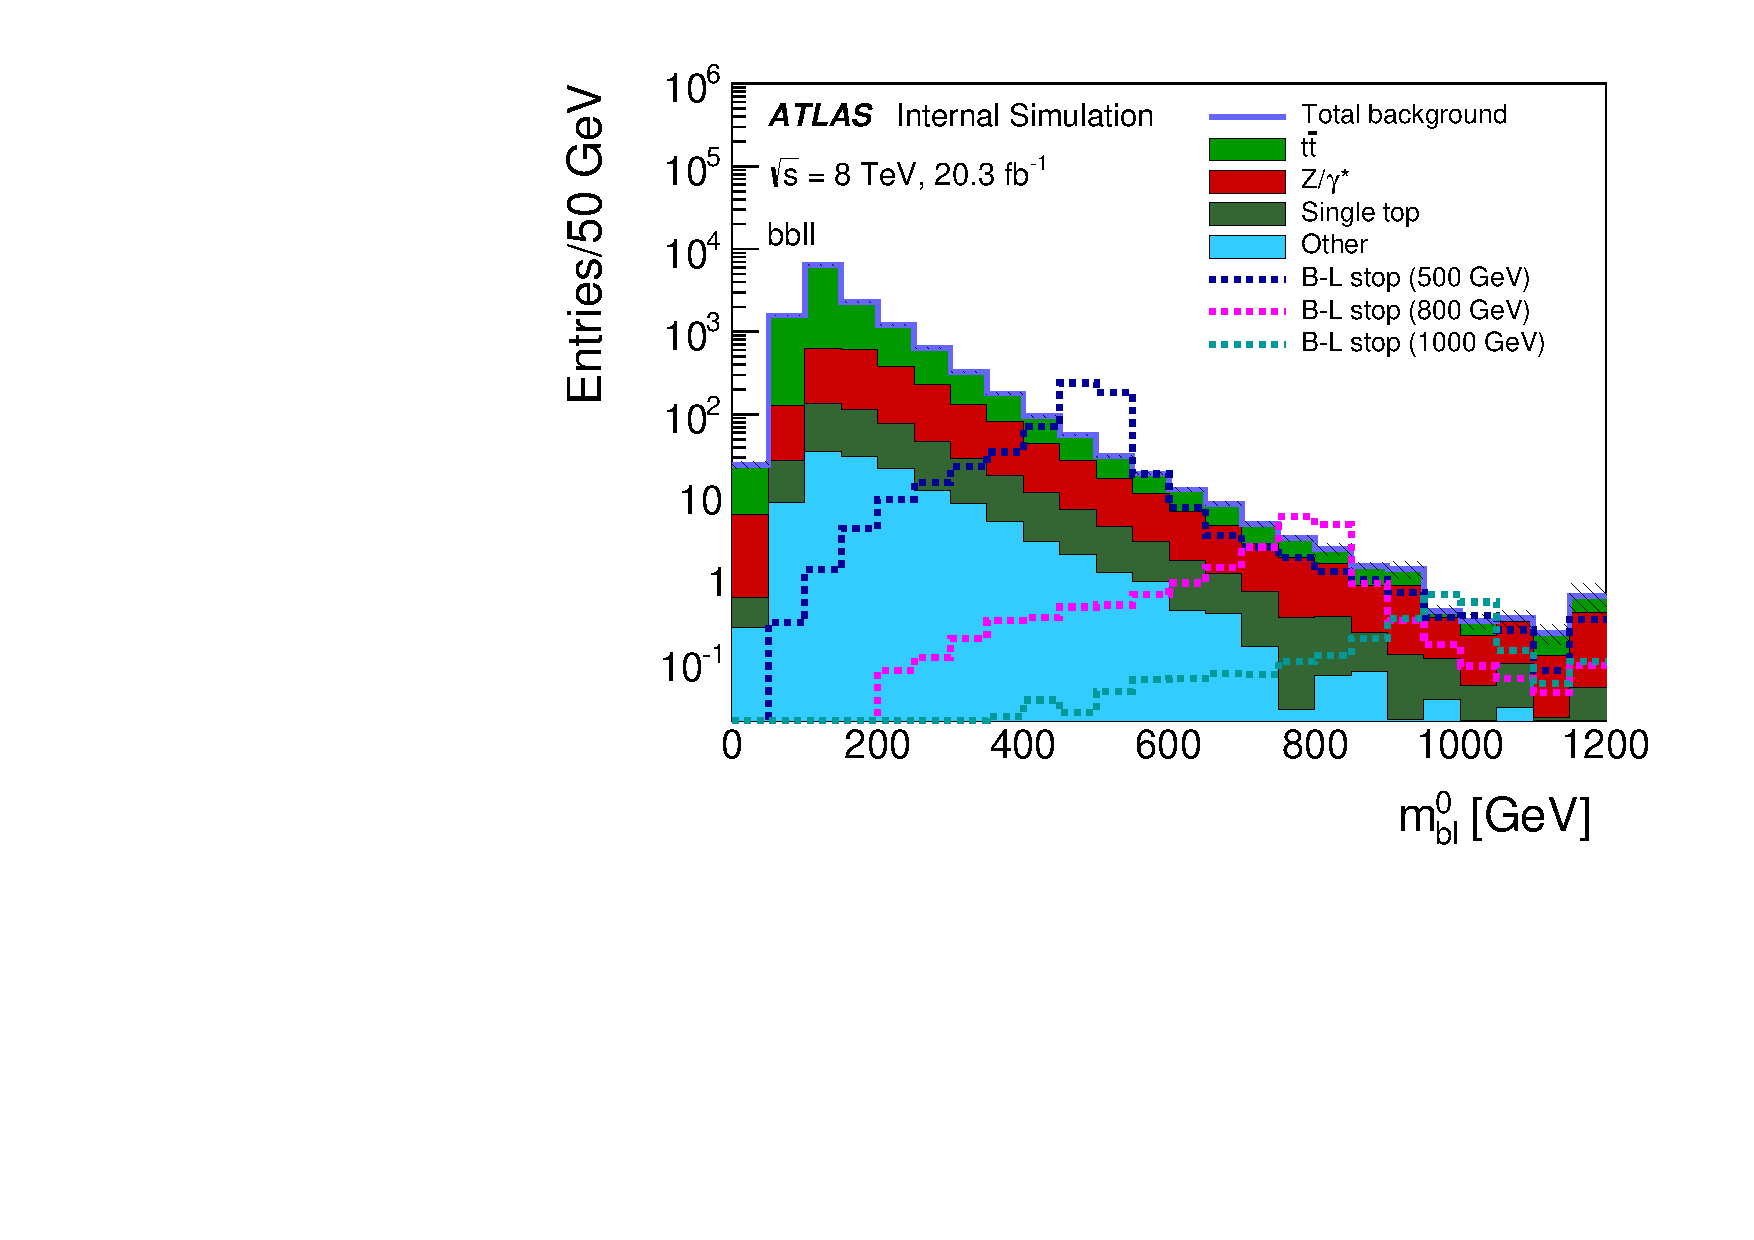
\includegraphics[width=0.48\textwidth, clip=true, trim=0 0 1cm 0]
    {figs/blstop/no_data__no_k_factor__dists/flavor_all__mbl_0__BMINUSL_BL_PAIRING__log.pdf}
  }
  \caption{Expected \MLL, \HT, \MBLASYM, and $\MBL^0$ distributions for SM
    background processes and three simulated stop samples with different masses.
    Basic event cleaning is applied and the events are required to pass the
    trigger selection, as described in
    Sections~\ref{sec:event_cleaning}~and~\ref{sec:trigger_selection}, and the
    events are required to have at least two $b$-tagged jets and two light
    leptons (electrons or muons).
    In each plot, the last bin includes the overflow for values beyond the
    maximum shown. The hashed error bands show only the statistical
    uncertainty on the background MC simulation samples. The signal
    models have an assumed
    $Br(\STOP\rightarrow~be)~=~Br(\STOP\rightarrow~b\mu)~=~0.5$.
  }
  \label{fig:no_data__no_k__inclusive_flavor_all__kinematic_dists}
  %%
\end{figure}

In order to achieve a large expected signal to background ratio in the signal
regions, MC simulation is used to optimize the selection requirements.
The optimization is performed assuming a stop branching fraction of
$Br(\STOP\rightarrow~be)~=~Br(\STOP\rightarrow~b\mu)~=~0.5$.
A single SR selection criteria is obtained for both the \HT\ and
\MBLASYM\ variables which perform reasonably well for all mass above 500 \GeV.
Events in both SRs are required to have $\HT \geq 1100~\GeV$ and
$\MBLASYM \leq 0.2$.
$\MBL^0$ is used to define the two SRs.
SR~400 has a requirement of $\MBL^0 \geq 400 \GeV$, and is optimal for lower
stop masses, while SR~600, with a requirement of $\MBL^0 \geq 600 \GeV$, is
optimal for higher stop masses.

Events in the SRs are required to have \HT\ above 1100~\GeV.
Events with two same-flavor leptons with invariant mass within 10~\GeV\ of the
$Z$-boson mass are vetoed to reduce the backgrounds from $Z$-boson production.
The SRs require a mass asymmetry of less than or equal to 0.2.
Finally, $\MBL^0$ is used to define the two SRs.
SR~400 has a requirement of $\MBL^0 \geq 400 \GeV$, and is optimal for lower
stop masses, while SR~600 has a requirement of $\MBL^0 \geq 600 \GeV$, and is
optimal for higher stop masses.
The full selection criteria for the analysis regions, including the Control and
Validation regions, described in Section~\ref{sec:bkg}, is outlined in
Table~\ref{tab:regions} and Figure~\ref{fig:region_coverage}.

%% - - - - - - - - - - - - - - - - - - - - - - - - - - - - - - - - - - - - - - -
\begin{table}[ht]
  \caption{Summary of signal, control, and validation regions used for this
    analysis.
    The control and validation regions are explained in Section~\ref{sec:bkg}.
    All regions require two $b$-tagged jets and two oppositely charged
    leptons. An event is in the $Z$ window if it contains two same-flavored
    leptons with an invariant mass within 10~\GeV\ of the mass of the $Z$ boson.
  }
  \label{tab:regions}
  %
  \centering{
    \begin{tabular}{l|ccccc}
      \toprule
      Region &
      $\MBL^0$ [\GeV] &
      \HT [\GeV] &
      \METSIG\ [$\GeV^{1/2}$] &
      \MBLASYM &
      $Z$ window \\
      \midrule
      SR~400   & $\geq 400$  & $\geq 1100$ & --       & $\leq 0.2$ & Veto   \\
      SR~600   & $\geq 600$  & $\geq 1100$ & --       & $\leq 0.2$ & Veto   \\
      \midrule
      Top CR   & $\geq 200$  & $\leq 500$  & $\geq 4$ & $\leq 0.2$ & Veto   \\
      $Z$ CR   & $\geq 200$  & $\leq 500$  & $\leq 4$ & $\leq 0.2$ & Select \\
      \midrule
      Top VR 1 & $\geq 200$  & $\leq 500$  & $< 4$    & $\leq 0.2$ & Veto   \\
      Top VR 2 & $\geq 200$  & $\leq 500$  & -        & $>    0.2$ & Veto   \\
      Top VR 3 & $\geq 200$  & $>   500$   & $> 4$    & $>    0.2$ & Veto   \\
      $Z$ VR   & $\geq 200$  & $>   500$   & --       & $\leq 0.2$ & Select \\
      \bottomrule
    \end{tabular}
  }
\end{table}

%% - - - - - - - - - - - - - - - - - - - - - - - - - - - - - - - - - - - - - - -
\begin{figure}[ht]
  \centering
  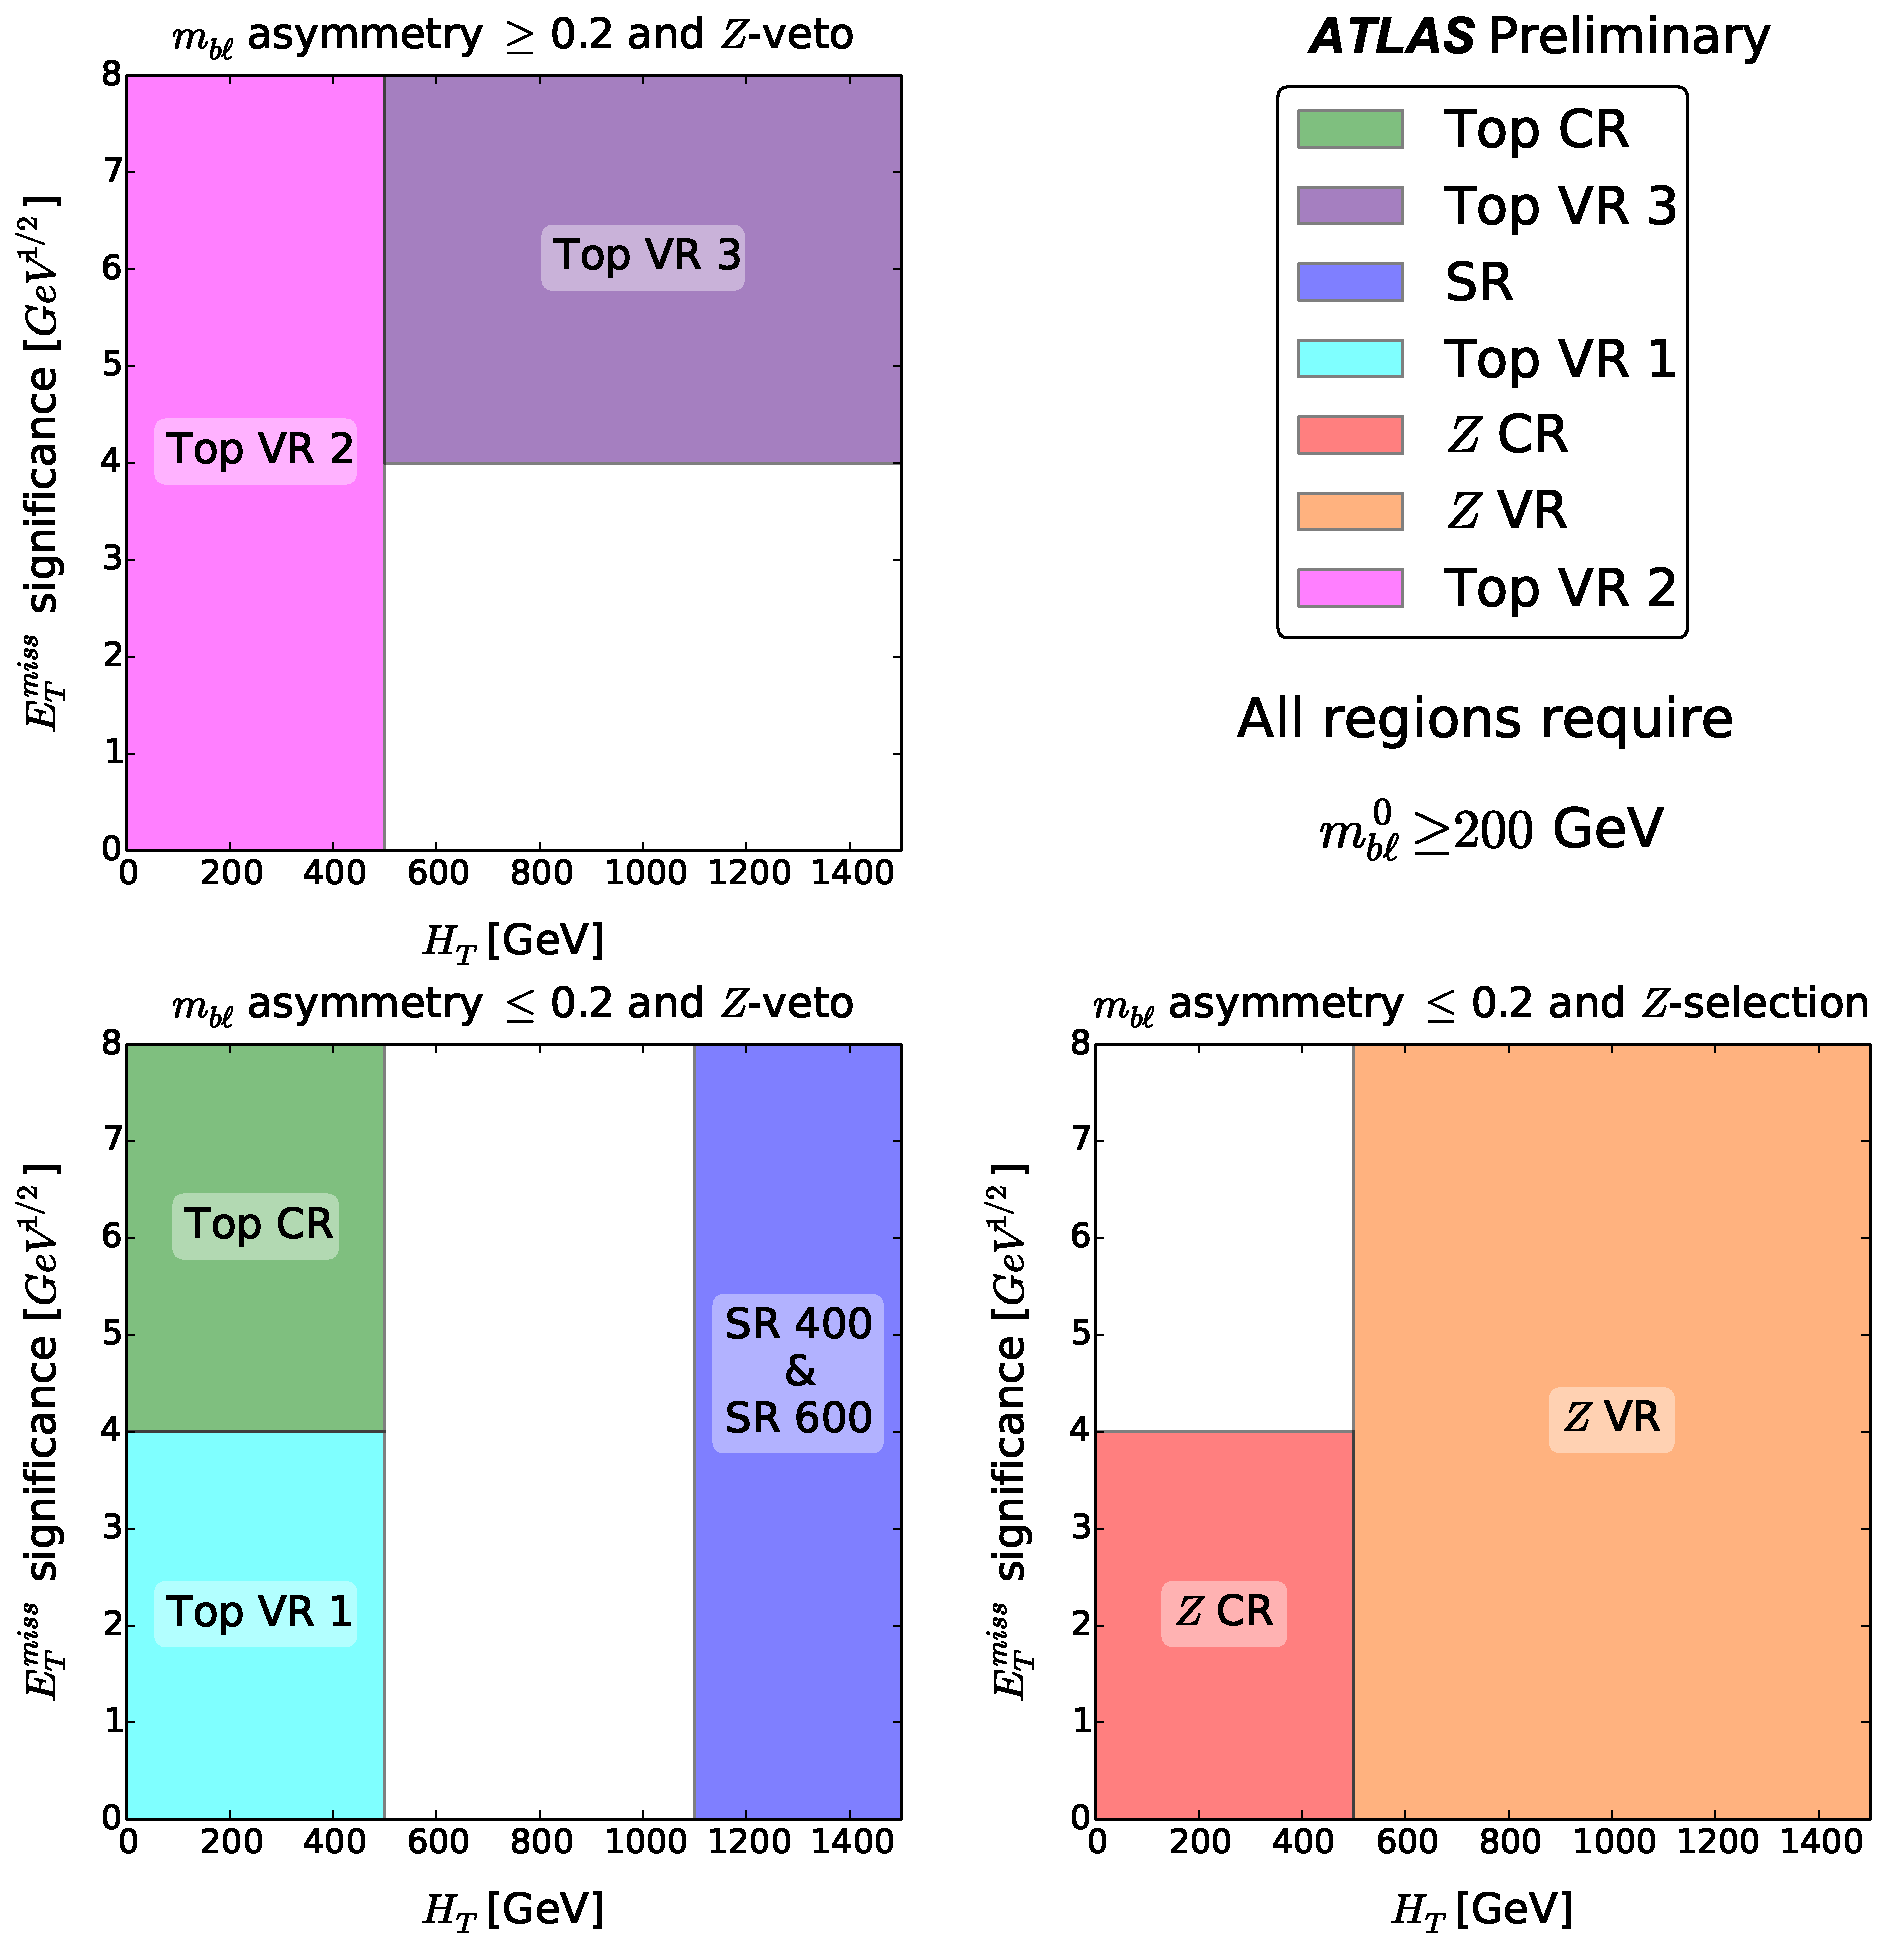
\includegraphics[width=\textwidth]{figs/blstop/regions__met_sig__ht_plane.pdf}
  \caption{Position of the regions in the \METSIG\ versus \HT\ space.
    The two left plots show the \METSIG-\HT~plane after vetoing events within
    the $Z$ window, with the top plot requiring $\MBLASYM \geq 0.2$ and the
    bottom requiring $\MBLASYM \leq 0.2$.
    The right plot shows the plane when requiring events be within the $Z$
    window.
    The two SRs apply a different requirement on the
    invariant mass of the higher-mass $b\ell$ pair. SR~400 requires
    $\MBL^{0} \geq 400 \GeV$, and SR~600 requires $\MBL^{0} \geq 600 \GeV$.
  }
  \label{fig:region_coverage}
\end{figure}

Figure~\ref{fig:n_minus_one_sr} shows the expected \HT, \MBLASYM, and $\MBL^0$
distributions after applying all the SR selection criteria except that on the
variable being shown.
This figure includes the simulated background processes and three signal models.
The number of expected signal events (for the same three signal models)
passing each selection requirement is shown in Table~\ref{tab:sr_cutflow}.
The estimates shown in Figure~\ref{fig:n_minus_one_sr} and
Table~\ref{tab:sr_cutflow} are taken from MC simulation, and the event
yields are normalized to 20.3 \ifb.

\begin{figure}
  \centering
  \subbottom[\HT]{
    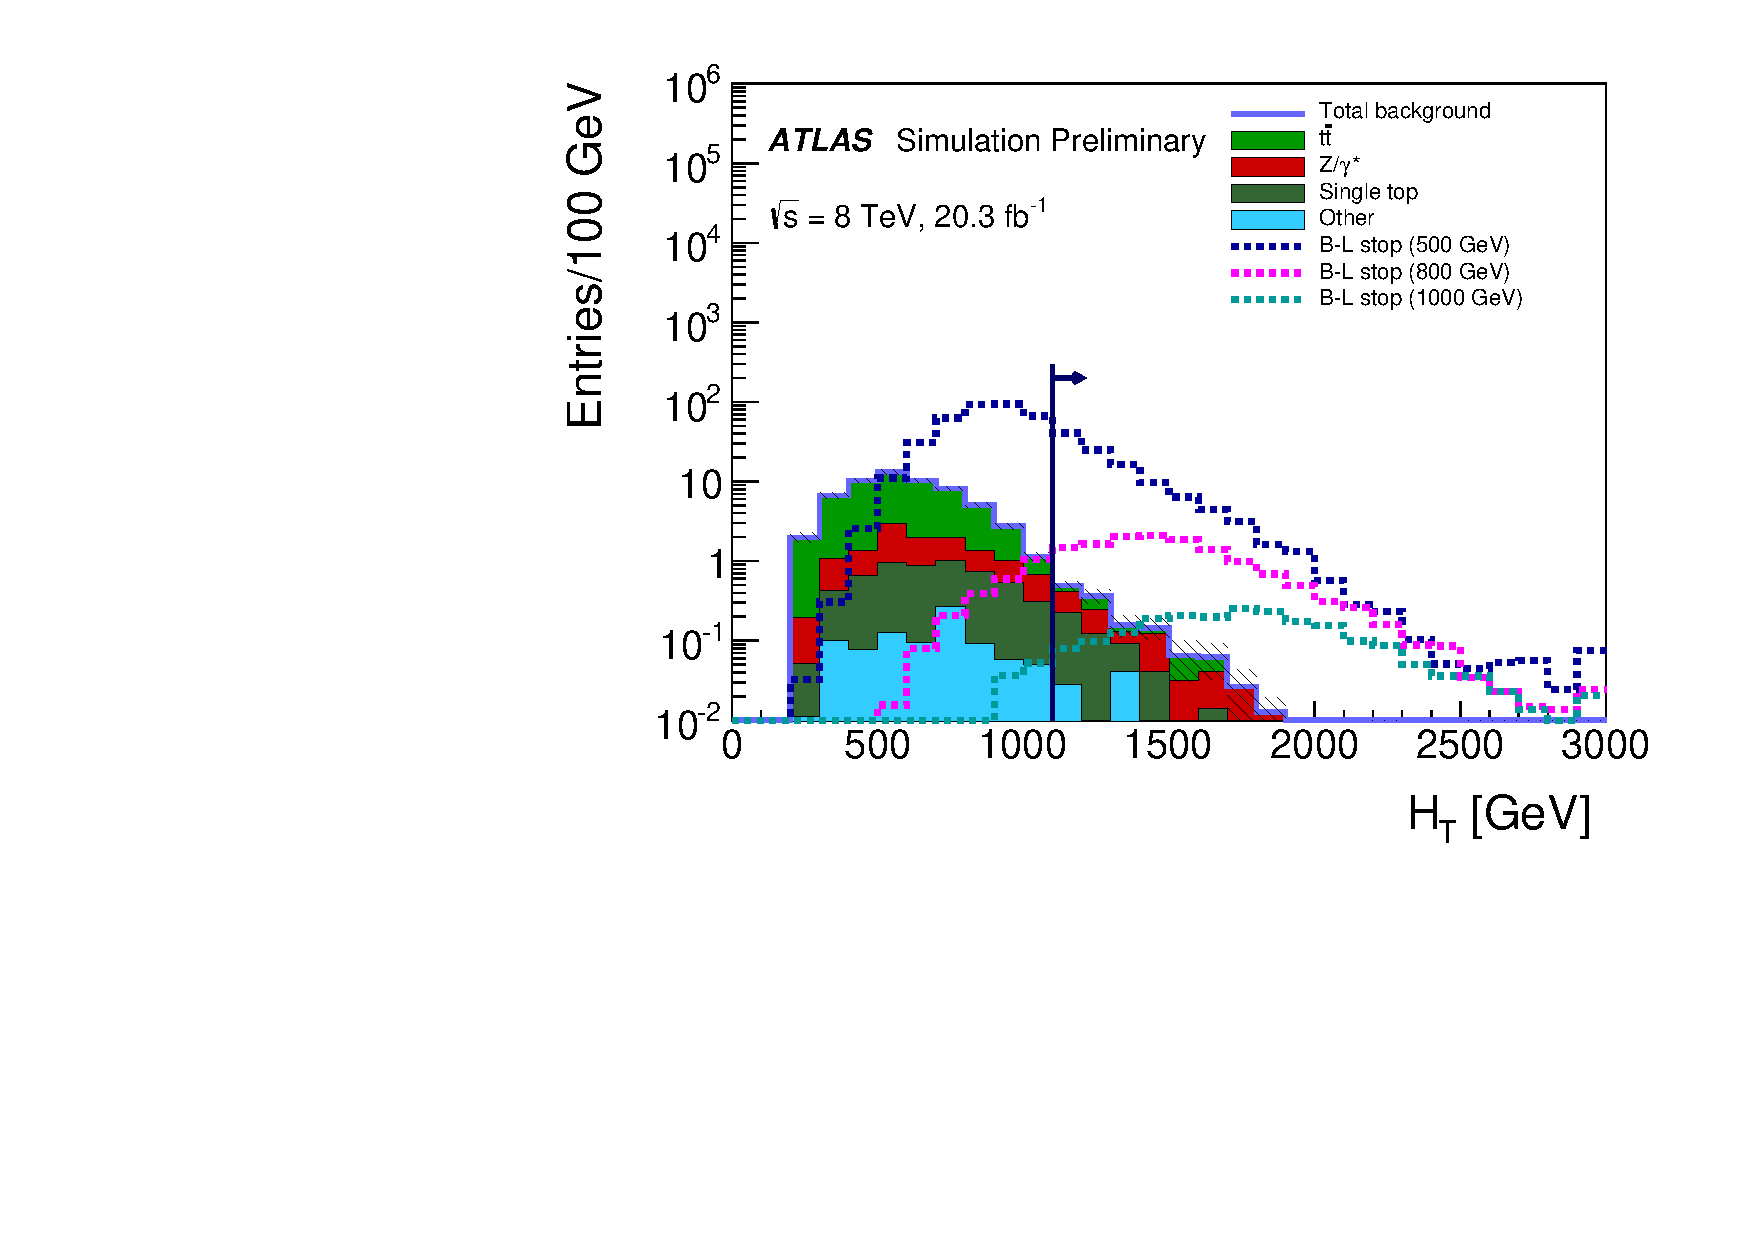
\includegraphics[width=0.48\textwidth, clip=true, trim=0 0 1cm 0]
      {figs/blstop/ht_sr_400_minus_ht.pdf}
  }
  \subbottom[\MBLASYM]{
    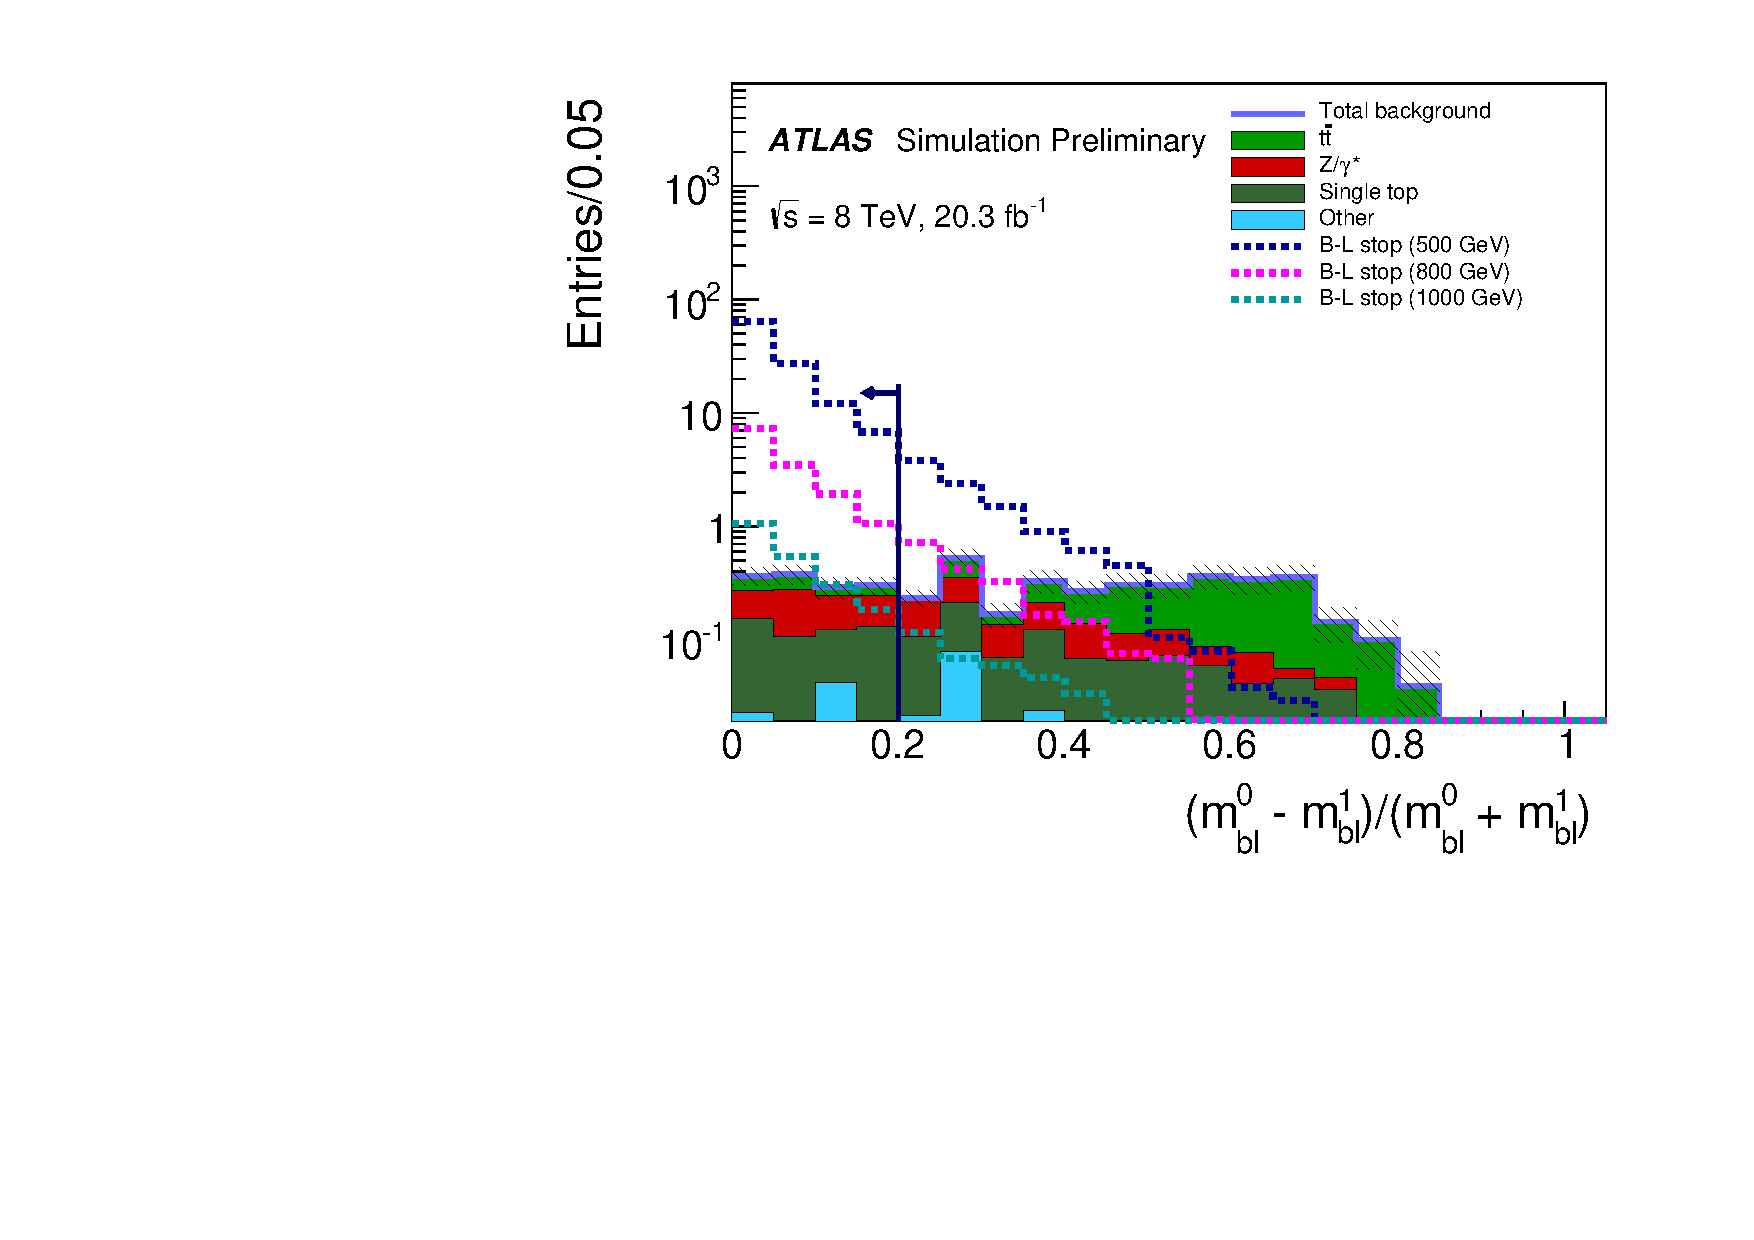
\includegraphics[width=0.48\textwidth, clip=true, trim=0 0 1cm 0]
      {figs/blstop/mbl_asym_sr_400_minus_mbl_asym.pdf}
  }
  \subbottom[$\MBL^0$]{
    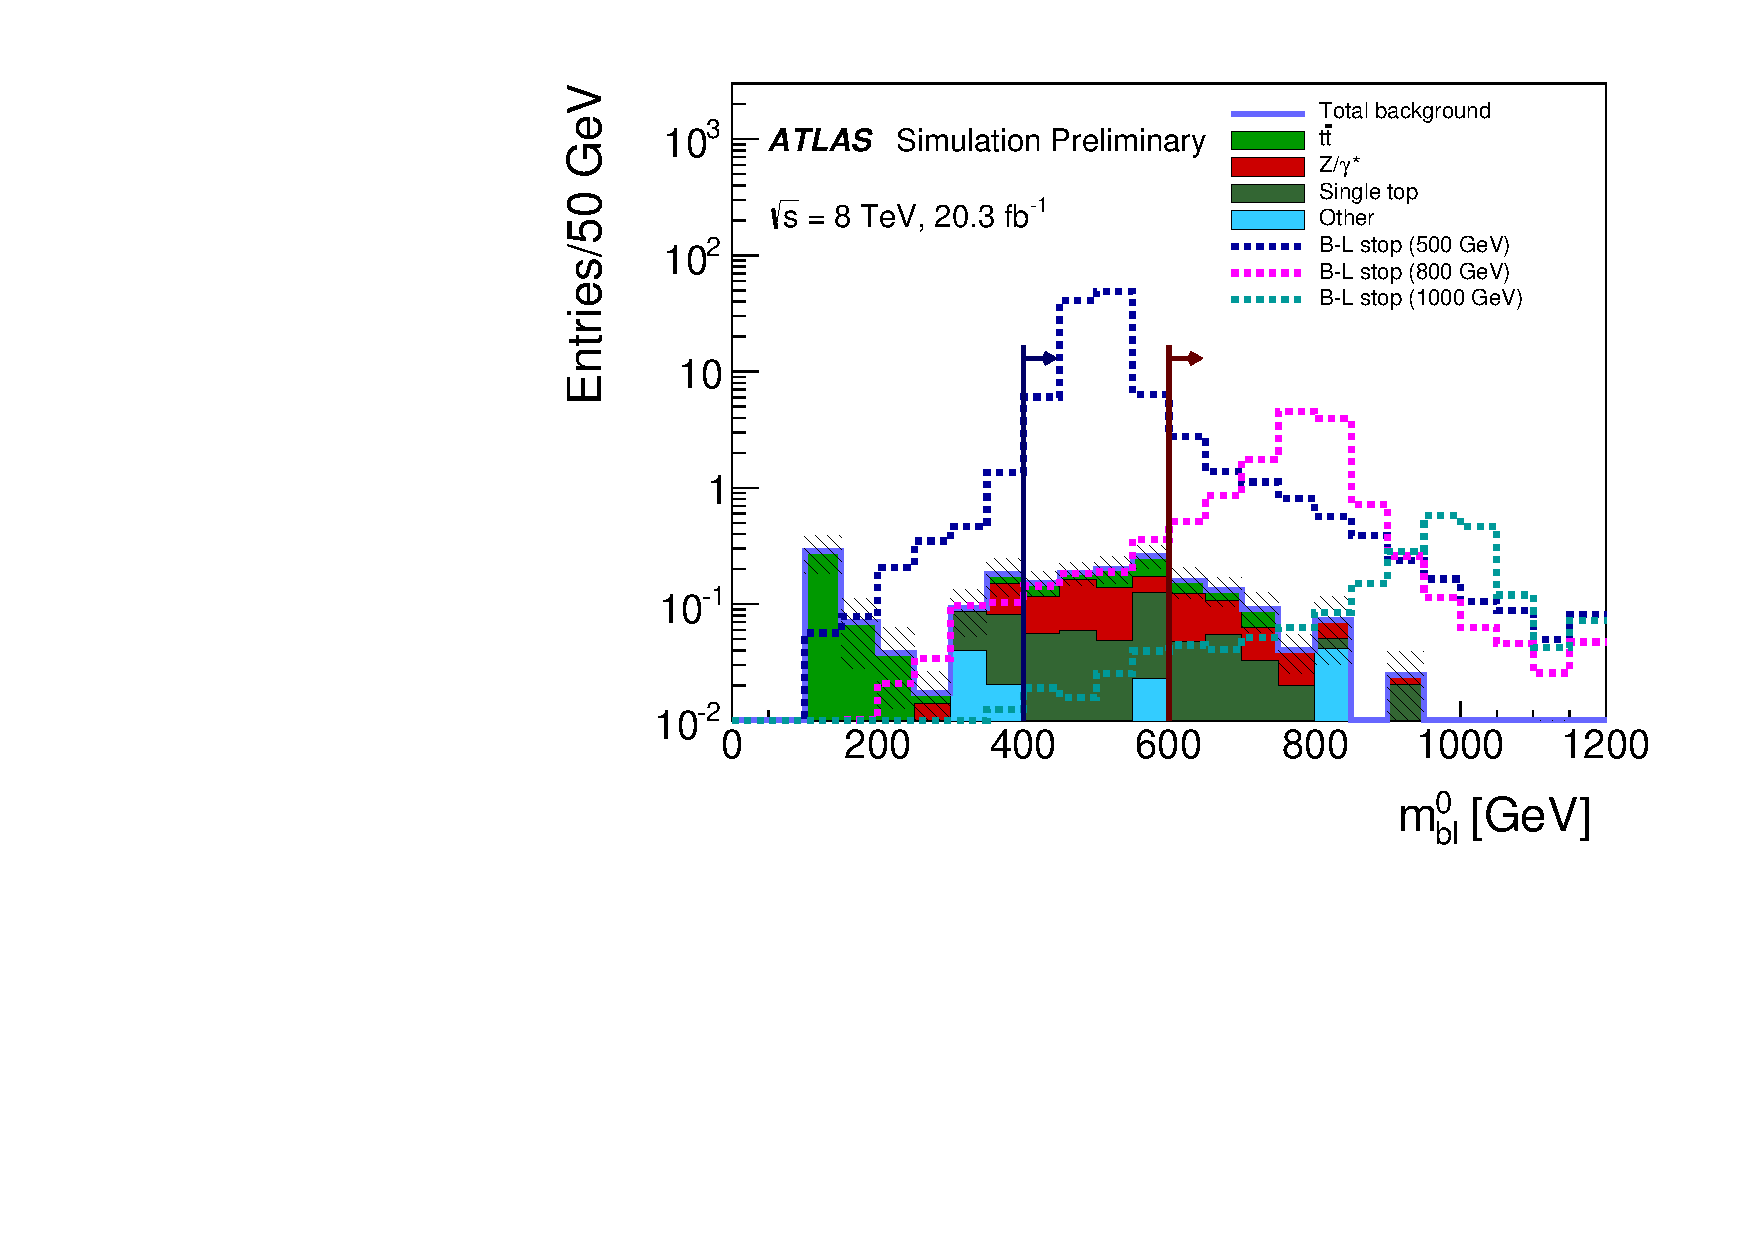
\includegraphics[width=0.48\textwidth, clip=true, trim=0 0 1cm 0]
      {figs/blstop/mbl_0_sr_minus_mbl.pdf}
  }
  \caption{Distributions of the variables which are used to define the SRs.
    These plots show the MC simulated background samples and three signal
    models, and are made after applying all the SR selection criteria except for
    that on the variable shown.
    The top two plots show the \HT\ and \MBLASYM\ variables, and the bottom
    plot shows the $\MBL^0$ distribution.
    The arrows show the SR requirement on the variable being shown.
    In each plot, the last bin includes the overflow for values beyond the
    maximum shown.
    The hashed error bands show only the statistical uncertainty on the
    background MC simulation samples.
    The signal models have an assumed
    $Br(\tilde{t}\rightarrow be) = Br(\tilde{t}\rightarrow b\mu) = 0.5$.
  }
  \label{fig:n_minus_one_sr}
  %%
\end{figure}

\begin{table}[ht]
  \caption{The number of expected signal events pasing each of the signal
    region cuts.
    This is shown for stop masses of 500~\GeV, 800~\GeV, and 1000~\GeV.
    The estimated yields are taken from MC simulation, and are normalized
    to 20.3~\ifb, and the uncertainty given is the MC statistical uncertainty.
    The signal models have an assumed branching fraction of
    $Br(\tilde{t}\rightarrow be) = Br(\tilde{t}\rightarrow b\mu) = 0.5$.
  }
  \label{tab:sr_cutflow}
  %
  \centering{
    \begin{tabular}{l|ccc}
      \toprule
      Selection                        & $m_{\tilde{t}} = 500 \GeV$ & $m_{\tilde{t}} = 800 \GeV$ & $m_{\tilde{t}} = 1000 \GeV$ \\
      \midrule
      $\sigma \cdot L$                 & $1750 \pm 260$             & $59 \pm 12$                & $8.9 \pm 2.5$ \\
      \midrule
      $bb\ell\ell$                     & $624 \pm 4$                & $19.65 \pm 0.18$           & $2.68 \pm 0.05$   \\
      $Z$ veto                         & $619 \pm 4$                & $19.62 \pm 0.18$           & $2.68 \pm 0.05$   \\
      $H_{T} \ge 1100 \GeV$            & $122.9 \pm 1.8$            & $16.01 \pm 0.17$           & $2.50 \pm 0.04$   \\
      $m_{b\ell}$ asymmetry $\leq 0.2$ & $112.8 \pm 1.7$            & $14.00 \pm 0.15$           & $2.11 \pm 0.04$   \\
      \midrule
      $m_{b\ell} \geq 400 \GeV$        & $110.3 \pm 1.7$            & $13.74 \pm 0.15$           & $2.09 \pm 0.04$   \\
      $m_{b\ell} \geq 600 \GeV$        & $7.7 \pm 0.4$              & $12.86 \pm 0.15$           & $1.99 \pm 0.04$   \\
      \bottomrule
    \end{tabular}
  }
\end{table}

%% -----------------------------------------------------------------------------
\section{Background estimate}
\label{sec:bkg}

The final state targeted by this analysis is two $b$-tagged jets and two light
leptons.
The three largest sources of SM background which contribute to this final state
are \TTBAR, \ZGAMMAJETS, and single top production.
Other sources, such as di-boson and Higgs boson production, contribute as
background events as well, however in much smaller amounts.
The full list of MC simulation samples used to estimate the background
contribution from SM processes is given in Section~\ref{sec:mc_samples}.
The background estimates for the \TTBAR\ and the \ZGAMMAJETS\ backgrounds use
MC simulation normalized in dedicated data control regions (CRs).
Several validation regions (VRs) are defined to validate the extrapolation of
the fitted background estimate in the CRs to regions with different kinematics.
The remaining backgrounds are estimated using MC simulation only, and the
normalization is scaled based on the cross section of the production process and
the integrated luminosity collected in data.
The CRs and VRs are described in more detail in
Sections~\ref{sec:cr}~and~\ref{sec:vr} respectively.

The \TTBAR\ and \ZGAMMAJETS\ normalization factors are determined using a
simultaneous fit to the data in th CRs, allowing the normalization of each
background to float independent of one another to obtain the best agreement
between the prediction and observation in the CRs.
The background fit procedure and results are described in
Section~\ref{sec:bkg_fit}.
In addition to the statistical uncertainty, several sources of systematic
uncertainty, described in Section~\ref{sec:systematics}, are considered when
performing the simultaneous fit.

%% -----------------------------------------------------------------------------
\subsection{Monte Carlo simulation samples}
\label{sec:mc_samples}

Monte Carlo simulation samples are used to estimate the selection efficiency
and kinematic distributions for SM processes.
When constructing plots and tables, the \TTBAR, \ZGAMMAJETS, and single top
production processes are kept separate, while all the other SM background
processes are grouped into an ``other'' category.
The \TTBAR\ background is modeled using the next-to-leading order (NLO)
generator \POWHEG\ 
revision~2129~\cite{Nason:2004rx, Frixione:2007vw, Alioli:2010xd,
Frixione:2007nw} with NLO PDF set CTEQ 6L1~\cite{Nadolsky:2008zw}, and 
showered with \PYTHIA\ version 6.426,
When using the baseline \POWHEG+\PYTHIA\ \TTBAR production sample,
events are reweighted in bins of the transverse mass (\pt) of the
$t\bar{t}$ system to match the top quark
pair differential cross section observed in ATLAS
data~\cite{Aad:2012hg,Aad:2014zka}.
The $Wt$-channel and $s$-channel of the single top background are
modeled using \POWHEG\ revision~1556~\cite{Alioli:2009je}
with \PYTHIA\ version 6.426, while the $t$-channel is modeled using
\acermc\ version 3.8~\cite{Kersevan:2004yg} with \PYTHIA\ version 6.426,
both with PDF set CTEQ 6L1~\cite{Nadolsky:2008zw}.
The \ZGAMMAJETS\ production process is modeled using
\SHERPA\ version~1.4.1~\cite{Gleisberg:2008ta} with NLO PDF set CT10.
Charm and bottom quarks are treated as massive.

The full list of background samples used, as well as the event generator used,
SM production cross section, and the effective luminosity generated is given in 
Tables~\ref{tab:background_grouping}, \ref{tab:background_grouping_z},
and \ref{tab:background_grouping_other}.\footnote{The effective luminosity is
given by $\nicefrac{N_\mathrm{gen}\sigma}{\epsilon_\mathrm{filter}}$, where
$N_\mathrm{gen}$ is the number of MC events which were generated, $\sigma$ is
the production cross section, and $\epsilon_\mathrm{filter}$ is the efficiency
of any filter which was applied to the MC sample.}
Unless \pythia8 is specified, \pythia\ version 6 is used for samples labeled
with \pythia.

\begin{table}[ht]
  \caption{Partial summary of background samples and their cross sections used
    in this analysis except for the \ZGAMMAJETS\ background (summarized in
    Table~\ref{tab:background_grouping_z}) and the "other" category (summarized
    in Table~\ref{tab:background_grouping_other})
  }
  \label{tab:background_grouping}
  \centering{
    \begin{tabular}{c|cccc}
      \toprule
      Grouping                    & Process      & Cross-section [pb] & Luminosity [$\mathrm{fb}^{-1}$] & Generator \\
      \midrule
      \TTBAR                      & \TTBAR       & 253                & 727.4                           & \powheg+\pythia \\
      \midrule
      \multirow{3}{*}{Single top} & $t$-channel  & 25.8               & 320                             & \acermc+\pythia \\
                                  & $s$-channel  & 1.64               & 330                             & \powheg+\pythia \\
                                  & $Wt$-channel & 2.15               & 4200                            & \powheg+\pythia \\
      \bottomrule
    \end{tabular}
  }
\end{table}


\begin{table}[ht]
  \caption{Summary of the \ZGAMMAJETS\ background samples and their cross
    sections used in this analysis.
    The \ZGAMMAJETS\ samples are sliced by the \pt\ of the $Z$ boson.
    For the inclusive sample, only events with $\pt^{Z} \le 40 \GeV$ were used.
    For each \pt\ slice, nine samples were generated, with different lepton
    flavor channels and filters applied on the jet flavor.
    The three samples are generated with approximately the same cross section,
    but the different filter efficiencies lead to different effective
    luminosities.
    The three columns under the effective luminosity represent the three
    samples.
    The left column shows the effective luminosity for the sample generated
    with a $b$-filter.
    The middle column represents the sample with a $c$-filter and $b$-veto.
    The right column shows the effective luminosity of the sample generated
    with a veto on both $b$- and $c$-quarks.
  }
  \label{tab:background_grouping_z}
  \centering{
    %% \resizebox{0.90\linewidth}{!}{
    %%   \begin{tabular}{c|cccccc}
    %%     \toprule
    %%     Grouping                       & Process                                                         & Cross-section [pb]   & \multicolumn{3}{c}{Luminosity [$\mathrm{fb}^{-1}$]} & Generator \\
    %%     \midrule
    %%     \multirow{24}{*}{\ZGAMMAJETS}  & $Z \rightarrow ee$                                              & 1110                 & 110                                                 & 9            & 6    & \sherpa \\
    %%                                    & $Z \rightarrow \mu\mu$                                          & 1110                 & 110                                                 & 9            & 6    & \sherpa \\
    %%                                    & $Z \rightarrow \tau\tau$                                        & 1110                 & 110                                                 & 9            & 6    & \sherpa \\
    %%                                    & $Z \rightarrow ee$        ($p_{T}^{Z} \in [40 ,70] \GeV$)       & 70.5                 & 110                                                 & 22           & 30   & \sherpa \\
    %%                                    & $Z \rightarrow \mu\mu$    ($p_{T}^{Z} \in [40 ,70] \GeV$)       & 70.5                 & 110                                                 & 22           & 30   & \sherpa \\
    %%                                    & $Z \rightarrow \tau\tau$  ($p_{T}^{Z} \in [40 ,70] \GeV$)       & 70.5                 & 110                                                 & 22           & 30   & \sherpa \\
    %%                                    & $Z \rightarrow ee$        ($p_{T}^{Z} \in [70 ,140] \GeV$)      & 29.5                 & 510                                                 & 90           & 110  & \sherpa \\
    %%                                    & $Z \rightarrow \mu\mu$    ($p_{T}^{Z} \in [70 ,140] \GeV$)      & 29.5                 & 510                                                 & 90           & 110  & \sherpa \\
    %%                                    & $Z \rightarrow \tau\tau$  ($p_{T}^{Z} \in [70 ,140] \GeV$)      & 29.5                 & 510                                                 & 90           & 110  & \sherpa \\
    %%                                    & $Z \rightarrow ee$        ($p_{T}^{Z} \in [140,280] \GeV$)      & 3.99                 & 470                                                 & 240          & 250  & \sherpa \\
    %%                                    & $Z \rightarrow \mu\mu$    ($p_{T}^{Z} \in [140,280] \GeV$)      & 3.99                 & 470                                                 & 240          & 250  & \sherpa \\
    %%                                    & $Z \rightarrow \tau\tau$  ($p_{T}^{Z} \in [140,280] \GeV$)      & 3.99                 & 470                                                 & 240          & 250  & \sherpa \\
    %%                                    & $Z \rightarrow ee$        ($p_{T}^{Z} \in [280,500] \GeV$)      & 0.24                 & 680                                                 & 480          & 360  & \sherpa \\
    %%                                    & $Z \rightarrow \mu\mu$    ($p_{T}^{Z} \in [280,500] \GeV$)      & 0.24                 & 680                                                 & 480          & 360  & \sherpa \\
    %%                                    & $Z \rightarrow \tau\tau$  ($p_{T}^{Z} \in [280,500] \GeV$)      & 0.24                 & 680                                                 & 480          & 360  & \sherpa \\
    %%                                    & $Z \rightarrow ee$        ($p_{T}^{Z} \ge 500 \GeV$)            & $1.3 \times 10^{-2}$ & 5700                                                & 1700         & 7000 & \sherpa \\
    %%                                    & $Z \rightarrow \mu\mu$    ($p_{T}^{Z} \ge 500 \GeV$)            & $1.3 \times 10^{-2}$ & 5700                                                & 1700         & 7000 & \sherpa \\
    %%                                    & $Z \rightarrow \tau\tau$  ($p_{T}^{Z} \ge 500 \GeV$)            & $1.3 \times 10^{-2}$ & 5700                                                & 1700         & 7000 & \sherpa \\
    %%                                    & DY $\rightarrow ee$       ($m_{Z/\gamma^{*}} \in [8 ,15] \GeV$) & 92.1                 & \multicolumn{3}{c}{50}                              & \sherpa \\
    %%                                    & DY $\rightarrow \mu\mu$   ($m_{Z/\gamma^{*}} \in [8 ,15] \GeV$) & 92.1                 & \multicolumn{3}{c}{50}                              & \sherpa \\
    %%                                    & DY $\rightarrow \tau\tau$ ($m_{Z/\gamma^{*}} \in [8 ,15] \GeV$) & 92.1                 & \multicolumn{3}{c}{50}                              & \sherpa \\
    %%                                    & DY $\rightarrow ee$       ($m_{Z/\gamma^{*}} \in [15,40] \GeV$) & 279                  & \multicolumn{3}{c}{50}                              & \sherpa \\
    %%                                    & DY $\rightarrow \mu\mu$   ($m_{Z/\gamma^{*}} \in [15,40] \GeV$) & 279                  & \multicolumn{3}{c}{50}                              & \sherpa \\
    %%                                    & DY $\rightarrow \tau\tau$ ($m_{Z/\gamma^{*}} \in [15,40] \GeV$) & 279                  & \multicolumn{3}{c}{50}                              & \sherpa \\
    %%     \bottomrule
    %%   \end{tabular}
    %% }
    % \resizebox{0.90\linewidth}{!}{
      \begin{tabular}{c|cccccc}
        \toprule
        Grouping                      & Process                                          & Cross-section [pb]                    & \multicolumn{3}{c}{Luminosity [$\mathrm{fb}^{-1}$]} & Generator \\
        \midrule
        \multirow{15}{*}{\ZGAMMAJETS} & $Z \rightarrow \ell\ell (ee, \mu\mu, \tau\tau)$  & 1110                                  & 110                                                 & 9                           & 6                     & \sherpa  \\ [1ex]
                                      & $Z \rightarrow \ell\ell (ee, \mu\mu, \tau\tau)$  & \multirow{2}{*}{70.5}                 & \multirow{2}{*}{110}                                & \multirow{2}{*}{22}         & \multirow{2}{*}{30}   & \multirow{2}{*}{\sherpa} \\
                                      & $p_{T}^{Z} \in [40 ,70] \GeV$                    & & & & &  \\ [1ex]
                                      & $Z \rightarrow \ell\ell (ee, \mu\mu, \tau\tau)$  & \multirow{2}{*}{29.5}                 & \multirow{2}{*}{510}                                & \multirow{2}{*}{90}         & \multirow{2}{*}{110}  & \multirow{2}{*}{\sherpa} \\
                                      & $p_{T}^{Z} \in [70 ,140] \GeV$                   & & & & &  \\ [1ex]
                                      & $Z \rightarrow \ell\ell (ee, \mu\mu, \tau\tau)$  & \multirow{2}{*}{3.99}                 & \multirow{2}{*}{470}                                & \multirow{2}{*}{240}        & \multirow{2}{*}{250}  & \multirow{2}{*}{\sherpa} \\
                                      & $p_{T}^{Z} \in [140,280] \GeV$                   & & & & &  \\ [1ex]
                                      & $Z \rightarrow \ell\ell (ee, \mu\mu, \tau\tau)$  & \multirow{2}{*}{0.24}                 & \multirow{2}{*}{680}                                & \multirow{2}{*}{480}        & \multirow{2}{*}{360}  & \multirow{2}{*}{\sherpa} \\
                                      & $p_{T}^{Z} \in [280,500] \GeV$                   & & & & &  \\ [1ex]
                                      & $Z \rightarrow \ell\ell (ee, \mu\mu, \tau\tau)$  & \multirow{2}{*}{$1.3 \times 10^{-2}$} & \multirow{2}{*}{5700}                               & \multirow{2}{*}{1700}       & \multirow{2}{*}{7000} & \multirow{2}{*}{\sherpa} \\
                                      & $p_{T}^{Z} \ge 500 \GeV$                         & & & & &  \\ [1ex]
                                      & DY $\rightarrow \ell\ell (ee, \mu\mu, \tau\tau)$ & \multirow{2}{*}{92.1}                 & \multicolumn{3}{c}{\multirow{2}{*}{50}}                                                                   & \multirow{2}{*}{\sherpa} \\
                                      & $m_{Z/\gamma^{*}} \in [8 ,15] \GeV$              & & & & &  \\ [1ex]
                                      & DY $\rightarrow \ell\ell (ee, \mu\mu, \tau\tau)$ & \multirow{2}{*}{279}                  & \multicolumn{3}{c}{\multirow{2}{*}{50}}                                                                   & \multirow{2}{*}{\sherpa} \\
                                      & $m_{Z/\gamma^{*}} \in [15,40] \GeV$              & & & & &  \\
        \bottomrule
      \end{tabular}
    % }
  }
\end{table}

\begin{table}[ht]
  \caption{Summary of other background samples and their cross sections used in
    this analysis.
    The $W \rightarrow \ell\nu$ and $Z \rightarrow \ell\ell$ processes each have 
    dedicated samples for each lepton flavor as indicated in the parentheses.
    The $W$ samples are generated with filters on the jet flavor.
    As in Table~\ref{tab:background_grouping_z}, the three columns under the
    effective luminosity represent the three samples ($b$-filter, $c$-filter
    and $b$-veto, veto on both $b$- and $c$-quarks).
  }
  \label{tab:background_grouping_other}
  \centering{
    %% \resizebox{0.90\linewidth}{!}{
    %%   \begin{tabular}{c|cccccc}
    %%     \toprule
    %%     Grouping &
    %%     Process &
    %%     Cross-section [pb] &
    %%     \multicolumn{3}{c}{Luminosity [$\mathrm{fb}^{-1}$]} &
    %%     Generator \\
    %%     \midrule
    %%     \multirow{50}{*}{Other}  & $\TTBAR\,W$                                                     & 0.10                 & \multicolumn{3}{c}{3300 }              & \madgraph+\pythia \\
    %%                              & $\TTBAR\,Wj$                                                    & $9.3 \times 10^{-2}$ & \multicolumn{3}{c}{3600 }              & \madgraph+\pythia \\
    %%                              & $\TTBAR\,Z$                                                     & $6.8 \times 10^{-2}$ & \multicolumn{3}{c}{4400 }              & \madgraph+\pythia \\
    %%                              & $\TTBAR\,Zj$                                                    & $8.7 \times 10^{-2}$ & \multicolumn{3}{c}{3400 }              & \madgraph+\pythia \\
    %%                              & $\TTBAR\,WW$                                                    & $9.2 \times 10^{-4}$ & \multicolumn{3}{c}{11000}              & \madgraph+\pythia \\
    %%                              & $WW \rightarrow \ell\ell\nu\nu$                                 & 5.30                 & \multicolumn{3}{c}{1400 }              & \sherpa           \\
    %%                              & $WW \rightarrow e\nu qq$                                        & 7.29                 & \multicolumn{3}{c}{100  }              & \sherpa           \\
    %%                              & $WW \rightarrow \mu\nu qq$                                      & 7.30                 & \multicolumn{3}{c}{100  }              & \sherpa           \\
    %%                              & $WW \rightarrow \tau\nu qq$                                     & 7.27                 & \multicolumn{3}{c}{100  }              & \sherpa           \\
    %%                              & $WZ \rightarrow \ell\ell\ell\nu$                                & 9.74                 & \multicolumn{3}{c}{260  }              & \sherpa           \\
    %%                              & $WZ \rightarrow \ell\nu\nu\nu$                                  & 1.40                 & \multicolumn{3}{c}{270  }              & \sherpa           \\
    %%                              & $WZ \rightarrow e\nu qq$                                        & 1.90                 & \multicolumn{3}{c}{110  }              & \sherpa           \\
    %%                              & $WZ \rightarrow \mu\nu qq$                                      & 1.91                 & \multicolumn{3}{c}{100  }              & \sherpa           \\
    %%                              & $WZ \rightarrow \tau\nu qq$                                     & 1.92                 & \multicolumn{3}{c}{100  }              & \sherpa           \\
    %%                              & $WZ \rightarrow ee qq$                                          & 1.46                 & \multicolumn{3}{c}{110  }              & \sherpa           \\
    %%                              & $WZ \rightarrow \mu\mu qq$                                      & 1.46                 & \multicolumn{3}{c}{110  }              & \sherpa           \\
    %%                              & $WZ \rightarrow \tau\tau qq$                                    & 1.45                 & \multicolumn{3}{c}{120  }              & \sherpa           \\
    %%                              & $WZ \rightarrow \nu\nu qq$                                      & 2.70                 & \multicolumn{3}{c}{64   }              & \sherpa           \\
    %%                              & $ZZ \rightarrow \ell\ell\nu\nu$                                 & 0.49                 & \multicolumn{3}{c}{1700 }              & \sherpa           \\
    %%                              & $ZZ \rightarrow ee qq$                                          & 0.25                 & \multicolumn{3}{c}{120  }              & \sherpa           \\
    %%                              & $ZZ \rightarrow \mu\mu qq$                                      & 0.25                 & \multicolumn{3}{c}{120  }              & \sherpa           \\
    %%                              & $ZZ \rightarrow \tau\tau qq$                                    & 0.24                 & \multicolumn{3}{c}{120  }              & \sherpa           \\
    %%                              & $ZZ \rightarrow \nu\nu qq$                                      & 1.74                 & \multicolumn{3}{c}{69   }              & \sherpa           \\
    %%                              & ggf $H \rightarrow WW$                                          & 0.44                 & \multicolumn{3}{c}{2000 }              & \powheg+\pythia 8 \\
    %%                              & ggf $H \rightarrow ZZ$                                          & $4.7 \times 10^{-2}$ & \multicolumn{3}{c}{2000 }              & \powheg+\pythia 8 \\
    %%                              & VBF $H \rightarrow WW$                                          & $3.6 \times 10^{-2}$ & \multicolumn{3}{c}{17000}              & \powheg+\pythia 8 \\
    %%                              & VBF $H \rightarrow ZZ$                                          & $3.8 \times 10^{-3}$ & \multicolumn{3}{c}{18000}              & \powheg+\pythia 8 \\
    %%                              & $WH \rightarrow W\ell\nu\ell\nu$                                & 0.15                 & \multicolumn{3}{c}{1000 }              & \pythia 8         \\
    %%                              & $WH \rightarrow W\ell\ell\nu\nu$                                & $1.7 \times 10^{-3}$ & \multicolumn{3}{c}{27000}              & \pythia 8         \\
    %%                              & $ZH \rightarrow Z\ell\nu\ell\nu$                                & $8.9 \times 10^{-3}$ & \multicolumn{3}{c}{2000 }              & \pythia 8         \\
    %%                              & $ZH \rightarrow Z\ell\ell\nu\nu$                                & $1.0 \times 10^{-2}$ & \multicolumn{3}{c}{48000}              & \pythia 8         \\
    %%                              & $\TTBAR H \rightarrow \TTBAR WW$                                & $2.8 \times 10^{-2}$ & \multicolumn{3}{c}{7000 }              & \pythia 8         \\
    %%                              & $W \rightarrow e\nu$                                            & 11000                & 100                       & 17   & 4   & \sherpa           \\
    %%                              & $W \rightarrow \mu\nu$                                          & 11000                & 100                       & 17   & 4   & \sherpa           \\
    %%                              & $W \rightarrow \tau\nu$                                         & 11000                & 100                       & 17   & 4   & \sherpa           \\
    %%                              & $W \rightarrow e\nu$    ($p_\mathrm{T}^{W} \in [40,70] \GeV$)   & 653                  & 44                        & 7    & 30  & \sherpa           \\
    %%                              & $W \rightarrow \mu\nu$  ($p_\mathrm{T}^{W} \in [40,70] \GeV$)   & 653                  & 44                        & 7    & 30  & \sherpa           \\
    %%                              & $W \rightarrow \tau\nu$ ($p_\mathrm{T}^{W} \in [40,70] \GeV$)   & 653                  & 44                        & 7    & 30  & \sherpa           \\
    %%                              & $W \rightarrow e\nu$    ($p_\mathrm{T}^{W} \in [70,140] \GeV$)  & 251                  & 160                       & 54   & 24  & \sherpa           \\
    %%                              & $W \rightarrow \mu\nu$  ($p_\mathrm{T}^{W} \in [70,140] \GeV$)  & 251                  & 160                       & 54   & 24  & \sherpa           \\
    %%                              & $W \rightarrow \tau\nu$ ($p_\mathrm{T}^{W} \in [70,140] \GeV$)  & 251                  & 160                       & 54   & 24  & \sherpa           \\
    %%                              & $W \rightarrow e\nu$    ($p_\mathrm{T}^{W} \in [140,280] \GeV$) & 31.2                 & 460                       & 260  & 80  & \sherpa           \\
    %%                              & $W \rightarrow \mu\nu$  ($p_\mathrm{T}^{W} \in [140,280] \GeV$) & 31.2                 & 460                       & 260  & 80  & \sherpa           \\
    %%                              & $W \rightarrow \tau\nu$ ($p_\mathrm{T}^{W} \in [140,280] \GeV$) & 31.2                 & 460                       & 260  & 80  & \sherpa           \\
    %%                              & $W \rightarrow e\nu$    ($p_\mathrm{T}^{W} \in [280,500] \GeV$) & 1.84                 & 590                       & 420  & 360 & \sherpa           \\
    %%                              & $W \rightarrow \mu\nu$  ($p_\mathrm{T}^{W} \in [280,500] \GeV$) & 1.84                 & 590                       & 420  & 360 & \sherpa           \\
    %%                              & $W \rightarrow \tau\nu$ ($p_\mathrm{T}^{W} \in [280,500] \GeV$) & 1.84                 & 590                       & 420  & 360 & \sherpa           \\
    %%                              & $W \rightarrow e\nu$    ($p_\mathrm{T}^{W} \ge 500 \GeV$)       & 0.10                 & 890                       & 360  & 140 & \sherpa           \\
    %%                              & $W \rightarrow \mu\nu$  ($p_\mathrm{T}^{W} \ge 500 \GeV$)       & 0.10                 & 890                       & 360  & 670 & \sherpa           \\
    %%                              & $W \rightarrow \tau\nu$ ($p_\mathrm{T}^{W} \ge 500 \GeV$)       & 0.10                 & 890                       & 360  & 670 & \sherpa           \\
    %%     \bottomrule
    %%   \end{tabular}
    %% }
      \begin{tabular}{c|cccccc}
        \toprule
        Grouping &
        Process &
        Cross-section [pb] &
        \multicolumn{3}{c}{Luminosity [$\mathrm{fb}^{-1}$]} &
        Generator \\
        \midrule
        \multirow{35}{*}{Other}    & $\TTBAR\,W$                                         & 0.10                  & \multicolumn{3}{c}{3300 } & \madgraph+\pythia \\
                                   & $\TTBAR\,Wj$                                        & $9.3 \times 10^{-2}$  & \multicolumn{3}{c}{3600 } & \madgraph+\pythia \\ [1ex]
                                   & $\TTBAR\,Z$                                         & $6.8 \times 10^{-2}$  & \multicolumn{3}{c}{4400 } & \madgraph+\pythia \\
                                   & $\TTBAR\,Zj$                                        & $8.7 \times 10^{-2}$  & \multicolumn{3}{c}{3400 } & \madgraph+\pythia \\ [1ex]
                                   & $\TTBAR\,WW$                                        & $9.2 \times 10^{-4}$  & \multicolumn{3}{c}{11000} & \madgraph+\pythia \\ [1ex]
                                   & $WW \rightarrow \ell\ell\nu\nu$                     & 5.30                  & \multicolumn{3}{c}{1400 } & \sherpa           \\
                                   & $WW \rightarrow \ell\nu qq (e,\mu,\tau)$            & 7.3                   & \multicolumn{3}{c}{100  } & \sherpa           \\ [1ex]
                                   & $WZ \rightarrow \ell\ell\ell\nu$                    & 9.74                  & \multicolumn{3}{c}{260  } & \sherpa           \\
                                   & $WZ \rightarrow \ell\nu\nu\nu$                      & 1.40                  & \multicolumn{3}{c}{270  } & \sherpa           \\
                                   & $WZ \rightarrow \ell\nu qq (e,\mu,\tau)$            & 1.9                   & \multicolumn{3}{c}{110  } & \sherpa           \\
                                   & $WZ \rightarrow \ell\ell qq (ee, \mu\mu, \tau\tau)$ & 1.46                  & \multicolumn{3}{c}{110  } & \sherpa           \\
                                   & $WZ \rightarrow \nu\nu qq$                          & 2.70                  & \multicolumn{3}{c}{64   } & \sherpa           \\ [1ex]
                                   & $ZZ \rightarrow \ell\ell\nu\nu$                     & 0.49                  & \multicolumn{3}{c}{1700 } & \sherpa           \\
                                   & $ZZ \rightarrow \ell\ell qq (ee, \mu\mu, \tau\tau)$ & 0.25                  & \multicolumn{3}{c}{120  } & \sherpa           \\
                                   & $ZZ \rightarrow \nu\nu qq$                          & 1.74                  & \multicolumn{3}{c}{69   } & \sherpa           \\ [1ex]
                                   & ggf $H \rightarrow WW$                              & 0.44                  & \multicolumn{3}{c}{2000 } & \powheg+\pythia 8 \\
                                   & ggf $H \rightarrow ZZ$                              & $4.7 \times 10^{-2}$  & \multicolumn{3}{c}{2000 } & \powheg+\pythia 8 \\
                                   & VBF $H \rightarrow WW$                              & $3.6 \times 10^{-2}$  & \multicolumn{3}{c}{17000} & \powheg+\pythia 8 \\
                                   & VBF $H \rightarrow ZZ$                              & $3.8 \times 10^{-3}$  & \multicolumn{3}{c}{18000} & \powheg+\pythia 8 \\ [1ex]
                                   & $WH \rightarrow W\ell\nu\ell\nu$                    & 0.15                  & \multicolumn{3}{c}{1000 } & \pythia 8         \\
                                   & $WH \rightarrow W\ell\ell\nu\nu$                    & $1.7 \times 10^{-3}$  & \multicolumn{3}{c}{27000} & \pythia 8         \\ [1ex]
                                   & $ZH \rightarrow Z\ell\nu\ell\nu$                    & $8.9 \times 10^{-3}$  & \multicolumn{3}{c}{2000 } & \pythia 8         \\
                                   & $ZH \rightarrow Z\ell\ell\nu\nu$                    & $1.0 \times 10^{-2}$  & \multicolumn{3}{c}{48000} & \pythia 8         \\ [1ex]
                                   & $\TTBAR H \rightarrow \TTBAR WW$                    & $2.8 \times 10^{-2}$  & \multicolumn{3}{c}{7000 } & \pythia 8         \\ [1ex]
                                   & $W \rightarrow \ell\nu (e, \mu, \tau)$              & 11000                 & 100                       & 17                   & 4                    & \sherpa \\ [1ex]
                                   & $W \rightarrow \ell\nu (e, \mu, \tau)$              & \multirow{2}{*}{653}  & \multirow{2}{*}{44}       & \multirow{2}{*}{7}   & \multirow{2}{*}{30}  & \multirow{2}{*}{\sherpa} \\
                                   & $p_\mathrm{T}^{W} \in [40,70] \GeV$                 &                       &                           &                      &                      & \\ [1ex]
                                   & $W \rightarrow \ell\nu (e, \mu, \tau)$              & \multirow{2}{*}{251}  & \multirow{2}{*}{160}      & \multirow{2}{*}{54}  & \multirow{2}{*}{24}  & \multirow{2}{*}{\sherpa} \\
                                   & $p_\mathrm{T}^{W} \in [70,140] \GeV$                &                       &                           &                      &                      & \\ [1ex]
                                   & $W \rightarrow \ell\nu (e, \mu, \tau)$              & \multirow{2}{*}{31.2} & \multirow{2}{*}{460}      & \multirow{2}{*}{260} & \multirow{2}{*}{80}  & \multirow{2}{*}{\sherpa} \\
                                   & $p_\mathrm{T}^{W} \in [140,280] \GeV$               &                       &                           &                      &                      & \\ [1ex]
                                   & $W \rightarrow \ell\nu (e, \mu, \tau)$              & \multirow{2}{*}{1.84} & \multirow{2}{*}{590}      & \multirow{2}{*}{420} & \multirow{2}{*}{360} & \multirow{2}{*}{\sherpa} \\
                                   & $p_\mathrm{T}^{W} \in [280,500] \GeV$               &                       &                           &                      &                      & \\ [1ex]
                                   & $W \rightarrow \ell\nu (e, \mu, \tau)$              & \multirow{2}{*}{0.10} & \multirow{2}{*}{890}      & \multirow{2}{*}{360} & \multirow{2}{*}{140} & \multirow{2}{*}{\sherpa} \\
                                   & $p_\mathrm{T}^{W} \ge 500 \GeV$                     &                       &                           &                      &                      &  \\
        \bottomrule
      \end{tabular}
  }
\end{table}

\FloatBarrier


%% -----------------------------------------------------------------------------
\subsection{Control regions}
\label{sec:cr}

The normalization of the \TTBAR\ and \ZGAMMAJETS\ backgrounds are determined
using the observed data in two dedicated CRs, labeled the top control region
(Top CR) and $Z$ control region ($Z$ CR) respectively.
To reduce the uncertainty on the \TTBAR\ and \ZGAMMAJETS\ normalization factors,
the CRs are defined to contain a fairly pure in events coming from a single
background process of interest.
The Top ($Z$) CR is defined to be pure in events from \TTBAR (\ZGAMMAJETS).
There is also little signal contamination in the CRs to prevent any potential
signal events from influencing the background normalization.

To reduce signal contamination, the Top and $Z$ CRs require $\HT \leq 500~\GeV$.
In addition to reducing the amount of signal contamination, the CRs should have
kinematics as similar as possible to the SRs to make the extrapolation from the
CRs to SRs more reliable.
For this reason, a requirement of $\MBLASYM \leq 0.2$ is applied to both the
Top and $Z$ CRs to match the \MBLASYM\ requirement in the SRs.
A requirement of $\MBL^0 \geq 200 \GeV$ is applied so the background
normalization is taken from a region of $\MBL^0$ which is more similar to that
of the SRs.
Imposing a stricter requirement on $\MBL^0$ reduces the expected and observed
number of events in both CRs, and a reliable estimate of the \TTBAR\ and
\ZGAMMAJETS\ normalizations cannot be obtained due to statistical uncertainties.
No requirement is made on the $\MBL^1$.

To ensure the CRs are relative in \TTBAR\ or \ZGAMMAJETS, the \MET\ information
is used.
Rather than select on the \MET\ alone, \METSIG\ is defined as
\begin{equation}
  \METSIG = \frac{\MET}{\sqrt{\HT}}.
\end{equation}
By scaling the \MET\ by the total amount of energy in the event, the
\METSIG\ is less susceptible to the effects of fake \MET\ from of mismeasurement
of objects in an event.
Processes like \TTBAR\ and single top, with real \MET\ in the final state, tend
to have large \METSIG, while processes with \MET coming entirely from
mismeasurement, such as \ZGAMMAJETS, tend to have low values for \METSIG.
For this reason, the Top CR requires $\METSIG \geq 4 \GeV^{1/2}$
and the $Z$ CR requires $\METSIG \leq 4 \GeV^{1/2}$.

Lastly, events containing like-flavor leptons, with a reconstructed invariant
mass within 10~\GeV of the $Z$~boson mass are rejected from the Top CR.
The $Z$ CR, requires events be within this $Z$ region.
The definitions of the CRs are summarized in Table~\ref{tab:regions} and
Figure~\ref{fig:region_coverage}.

The expected and observed $\MBL^{0}$ distributions in the Top CR and $Z$ CR,
shown in Figure~\ref{fig:cr_mbl_0__no_norm_factor} shows reasonable agreement
between the predicted and observed data in the Top CR, however, the
normalization is underpredicted in the $Z$ CR.
This disagreement seems to be caused by a poor modeling of the
\ZGAMMAJETS\ background process when heavy flavor jets are required in the
final state.
For the final result, the fit procedure is used to determine the normalization
of the \ZGAMMAJETS\ background; however, due to the large disagreement, it is
useful to scale the \ZGAMMAJETS\ background based on this disagreement for
exploratory plots and tables to obtain a more realistic estimate of the expected
backgrounds in each region.
This scaling factor is determined to be $k_Z = 1.39$, and will be applied to
many of the plots in this section.
This normalization factor is not included in the final fit to data, and any plot
or figure which is produced using this normalization factor will explicitly
states this in the description.

\begin{figure}
  \centering
  \subbottom[Top CR]{
    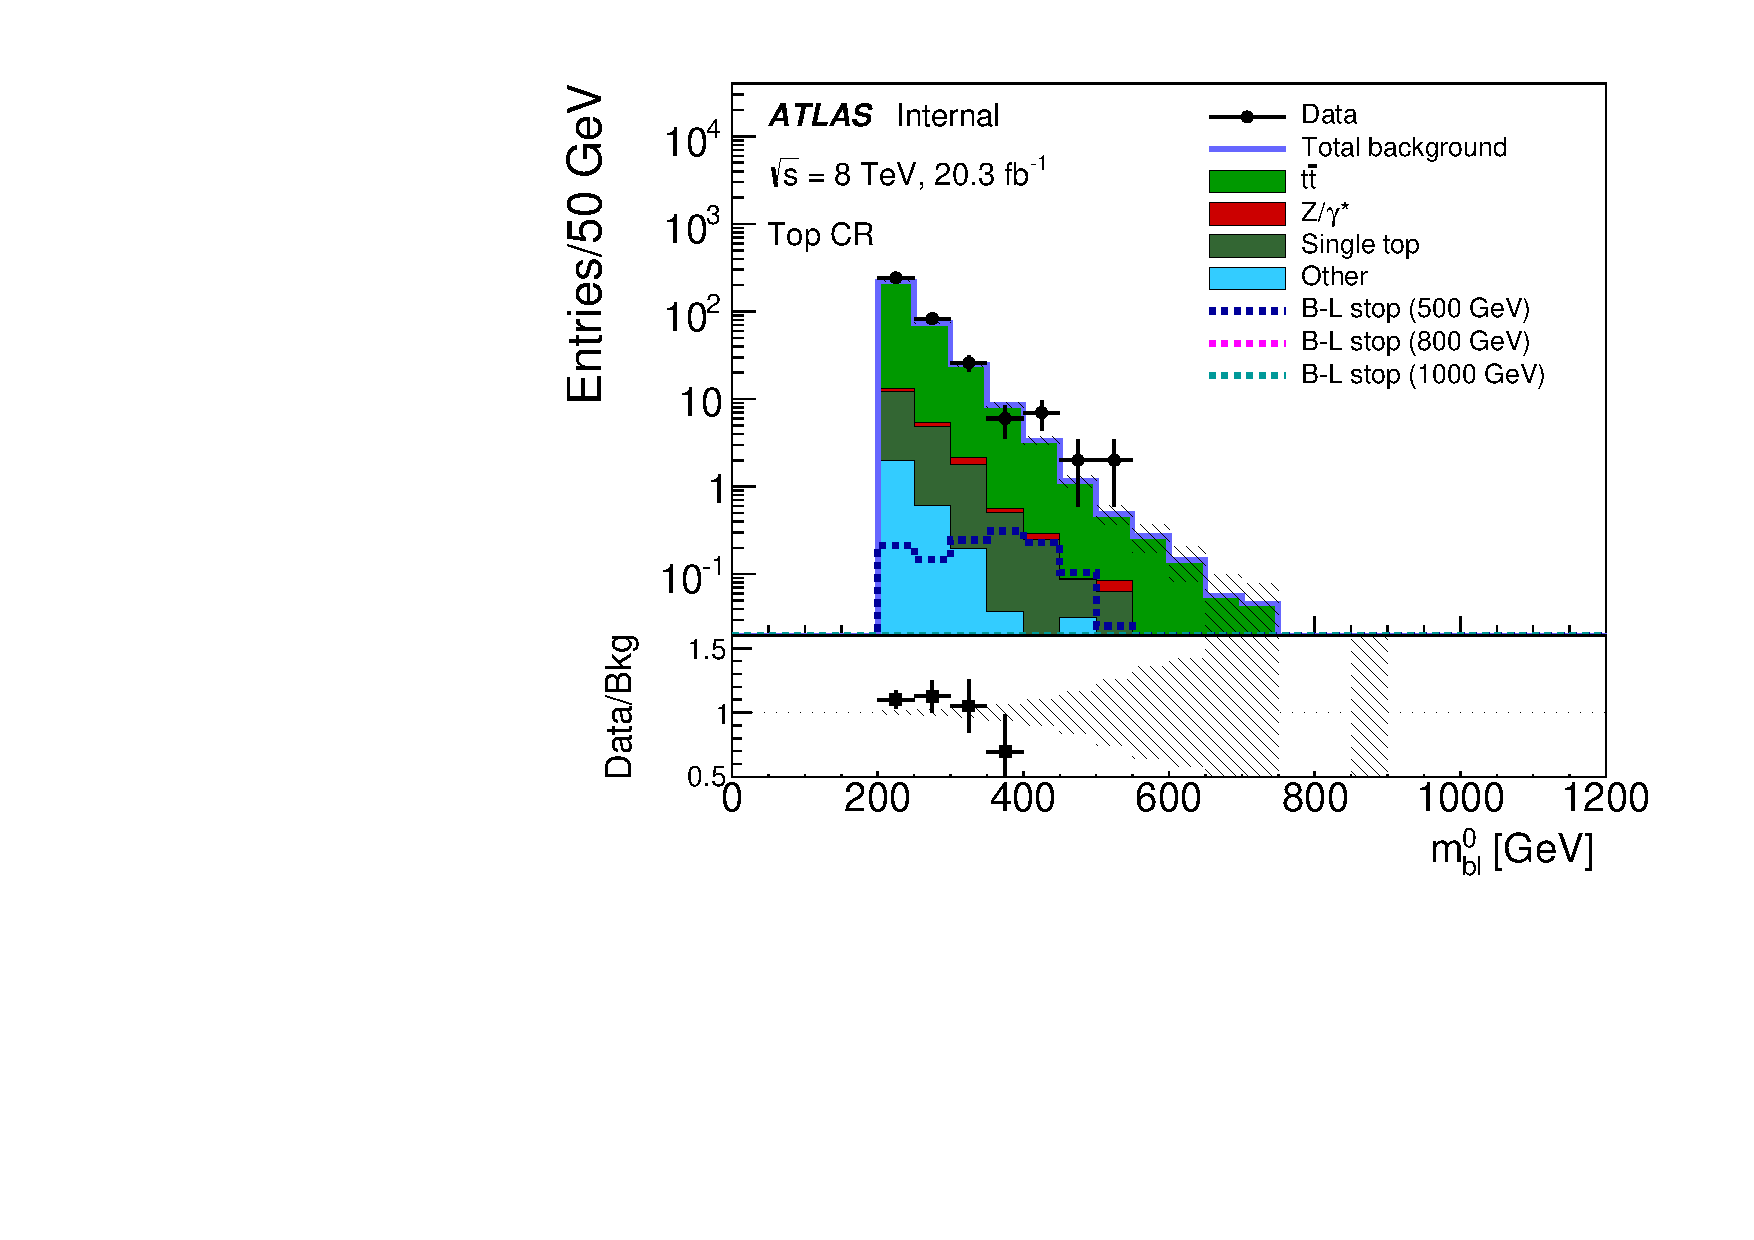
\includegraphics[width=0.48\textwidth, clip=true, trim=0 0 1cm 0]
      {figs/blstop/w_data__no_k_factor__dists/flavor_all__mbl_0__BMINUSL_CR_TOP_MBL_200__log.pdf}
  }
  \subbottom[$Z$ CR]{
    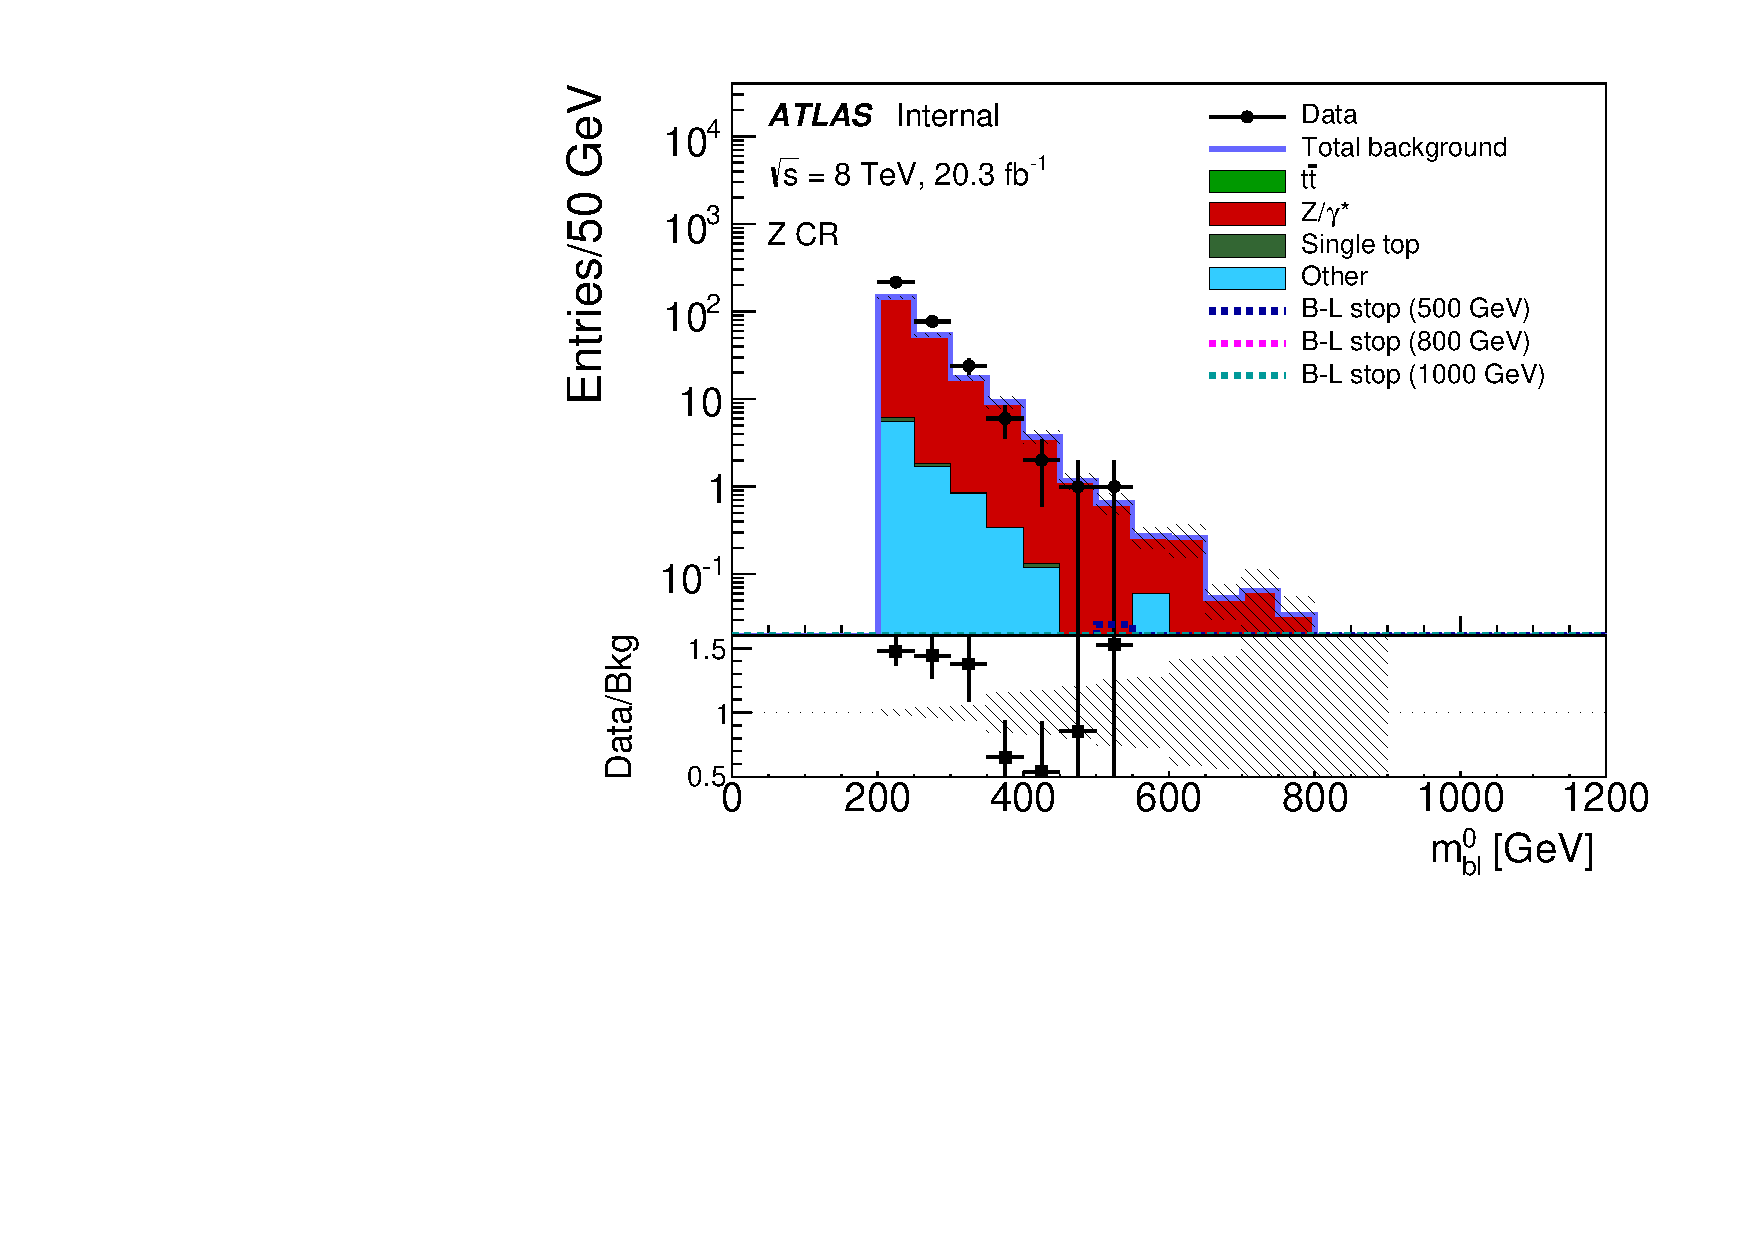
\includegraphics[width=0.48\textwidth, clip=true, trim=0 0 1cm 0]
      {figs/blstop/w_data__no_k_factor__dists/flavor_all__mbl_0__BMINUSL_CR_Z_MBL_200__log.pdf}
  }
  \caption{Expected and observed $\MBL^0$ distribution in the Top CR and
    $Z$ CR when all flavor channels are combined.
    The prediction in the Top CR shows reasonable agreement with the observed
    data.
    The background is underpredicted in the $Z$ CR.
    % In each plot, the last bin includes the overflow for values beyond the
    % maximum shown.
    The hashed error bands show only the statistical uncertainty on the
    background MC simulation samples.
    The signal models have an assumed
    $Br(\tilde{t}\rightarrow be) = Br(\tilde{t}\rightarrow b\mu) = 0.5$.
  }
  \label{fig:cr_mbl_0__no_norm_factor}
  %%
\end{figure}

After applying the $k_Z$ normalization factor the $\MBL^0$ distributions in
the Top CR and $Z$ CR are shown in Figure~\ref{fig:cr_mbl_0__w_norm_factor}.
While the prediction is roughly unchanged in the Top CR, the prediction in the
$Z$ CR shows much better agreement with the data.
The expected and observed event yields in the two CRs, broken out by background
production process, are shown in Table~\ref{tab:region_contributions_cr}.

\begin{figure}
  \centering
  \subbottom[Top CR]{
    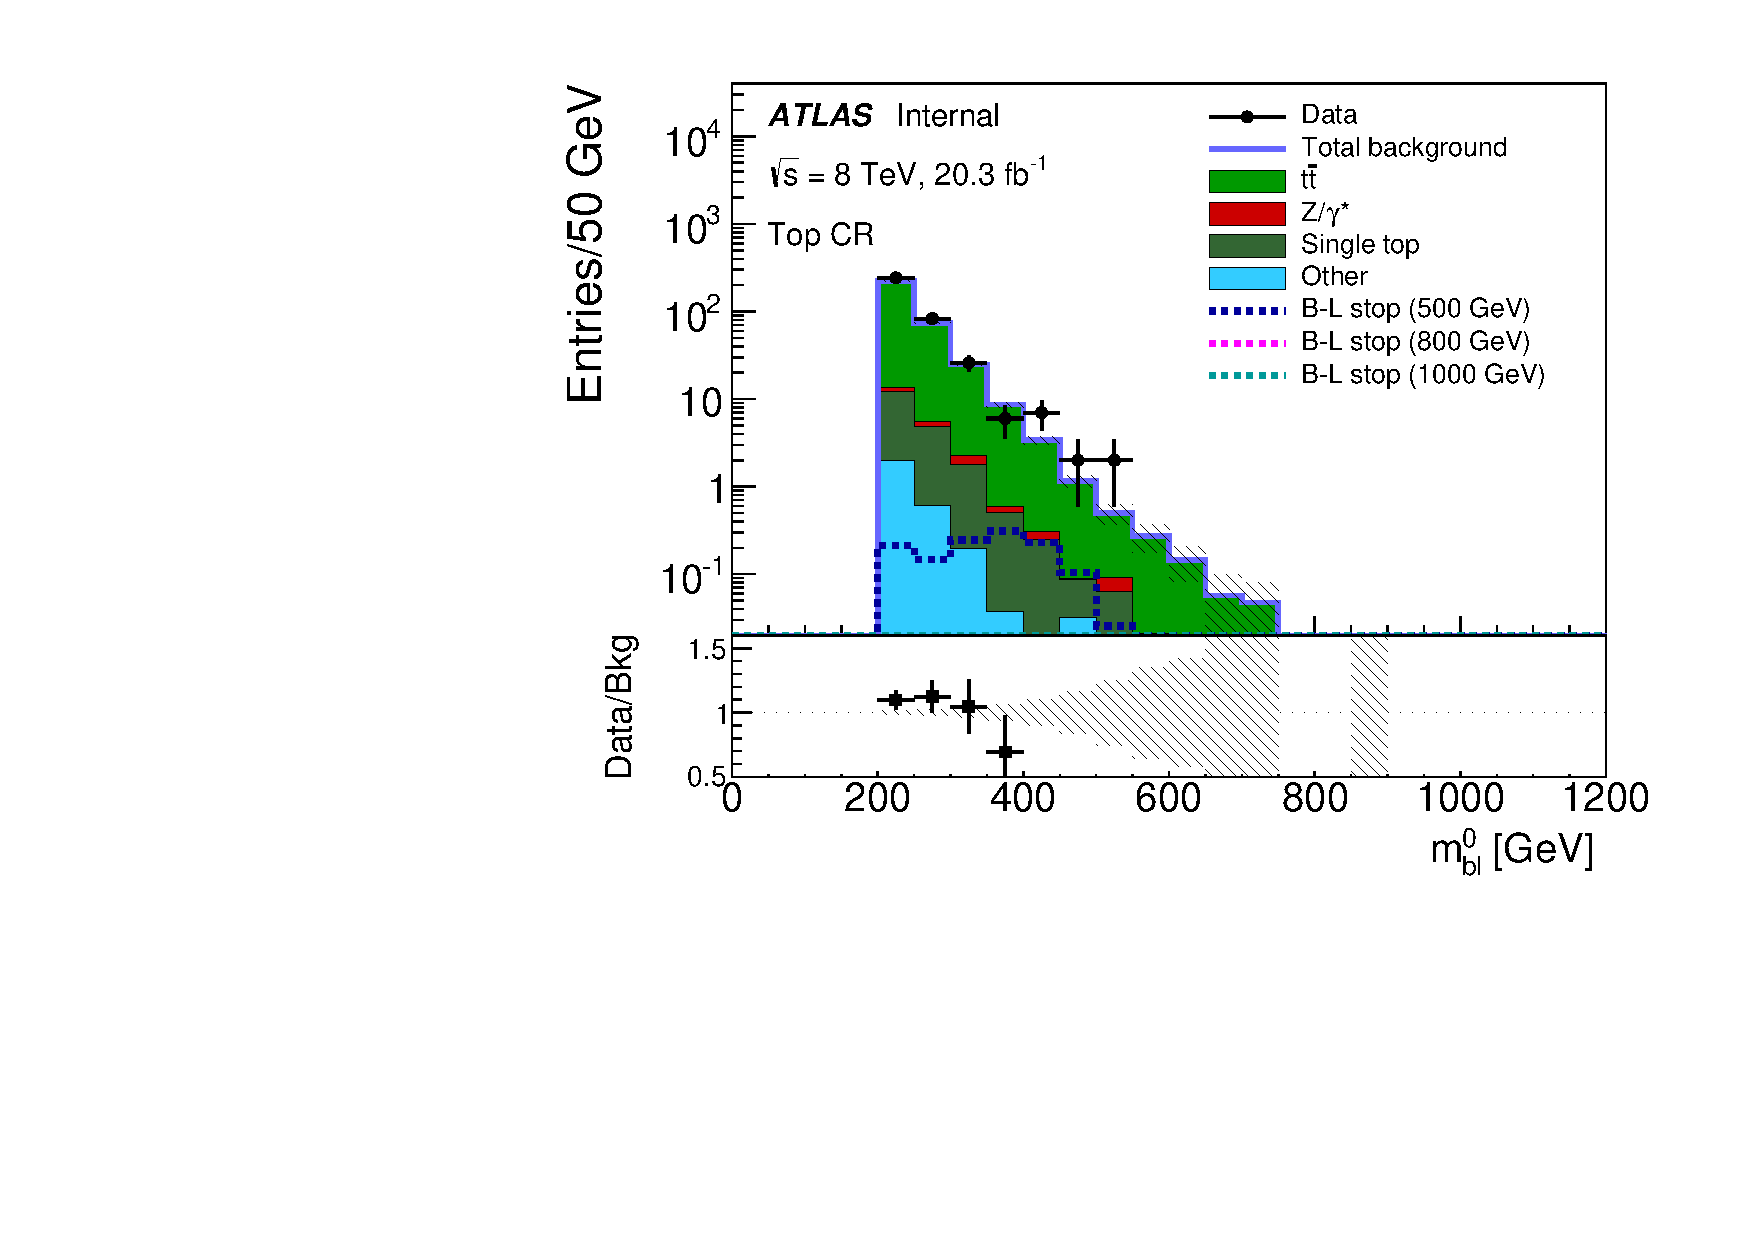
\includegraphics[width=0.48\textwidth, clip=true, trim=0 0 1cm 0]
      {figs/blstop/w_data__w_k_factor__dists/flavor_all__mbl_0__BMINUSL_CR_TOP_MBL_200__log.pdf}
  }
  \subbottom[$Z$ CR]{
    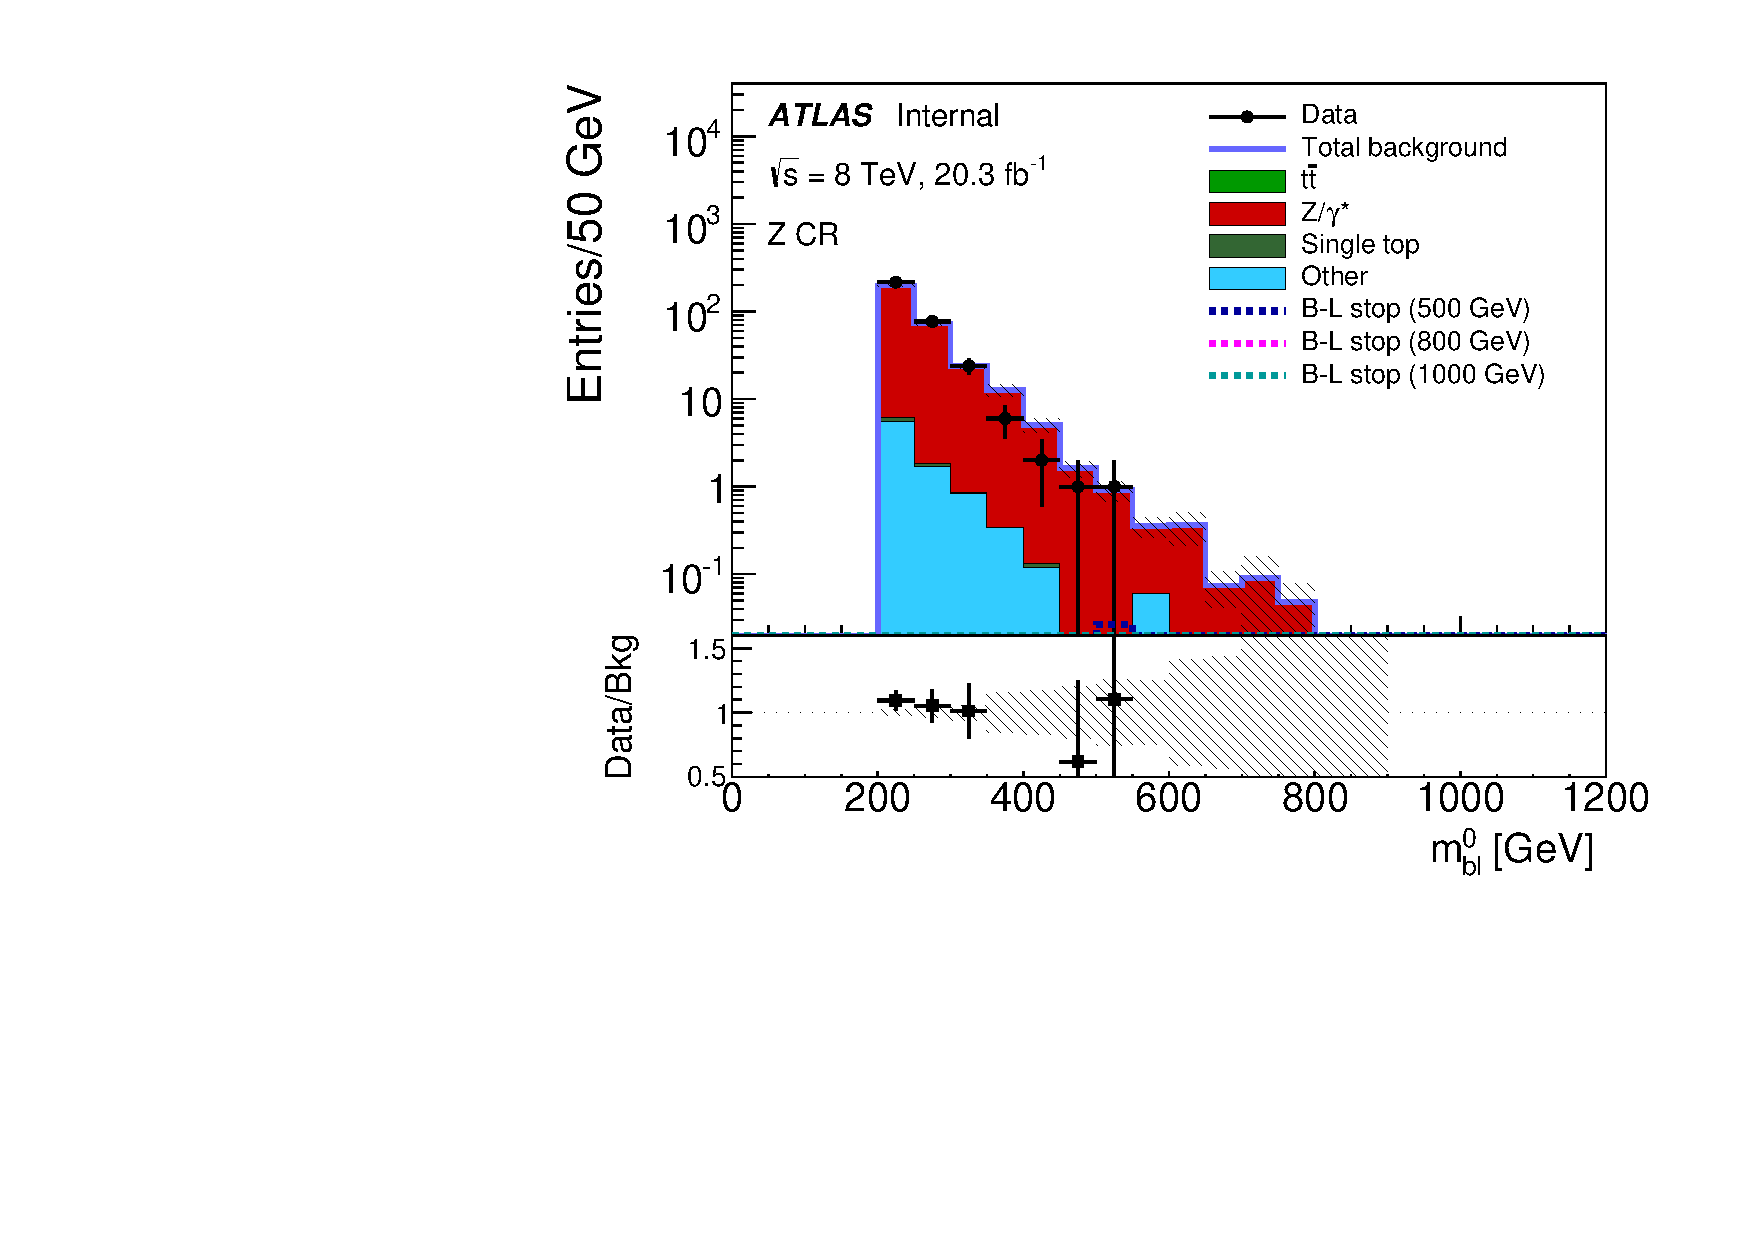
\includegraphics[width=0.48\textwidth, clip=true, trim=0 0 1cm 0]
      {figs/blstop/w_data__w_k_factor__dists/flavor_all__mbl_0__BMINUSL_CR_Z_MBL_200__log.pdf}
  }
  \caption{Expected and observed $\MBL^0$ distribution in the Top CR and
    $Z$ CR after applying the $k_Z$ normalization factor derived in the $Z$ CR
    when all flavor channels are combined.
    After applying the $k_Z$ normalization factor, both CRs show reasonable
    agreement between the predicted and observed distributions.
    % In each plot, the last bin includes the overflow for values beyond the
    % maximum shown.
    The hashed error bands show only the statistical uncertainty on the
    background MC simulation samples.
    The signal models have an assumed
    $Br(\tilde{t}\rightarrow be) = Br(\tilde{t}\rightarrow b\mu) = 0.5$.
  }
  \label{fig:cr_mbl_0__w_norm_factor}
  %%
\end{figure}

\begin{table}
  \caption{Number of expected events in each of the CRs broken down by process.
    The uncertainty on the total background prediction is the MC statistical
    uncertainty only for each background process.
    The total uncertainty is obtained by summing the uncertainty on each
    background process in quadrature.
    The $k_Z$ normalization factor is applied to the \ZGAMMAJETS\ background
    yield estimate.
    % For each signal model, the ratio of expected signal events to the sum of the
    % background in each region is show in parentheses.
    {\color{red} TODO add observed number events in each CR.}
    {\color{red} TODO update with only stat uncertainty.}
    {\color{red} TODO update with breakdown by flavor channel.}
  }
  \label{tab:region_contributions_cr}
  \centering{
    \begin{tabular}{c|cc}
      \toprule
                                           & Top CR                            & $Z$ CR                            \\
      \midrule
      \TTBAR                               & $311.8$                           & $8.2$                             \\
      \ZGAMMAJETS                          & $3.1$                             & $297.9$                           \\
      Single top                           & $16.7$                            & $0.8$                             \\
      Other                                & $2.9$                             & $8.6$                             \\
      \midrule
      Total                                & \multirow{2}{*}{$334.5 \pm 93.7$} & \multirow{2}{*}{$315.6 \pm 89.5$} \\
      background                           &                                   &                                   \\
      \midrule
      \multirow{2}{*}{B-L stop (500 GeV)}  & $1.3$                             & $0.03$                            \\
                                           & ($< 0.01$)                        & ($< 0.01$) \vspace{1ex}           \\
      \multirow{2}{*}{B-L stop (800 GeV)}  & $< 0.01$                          & $< 0.01$                          \\
                                           & ($< 0.01$)                        & ($< 0.01$) \vspace{1ex}           \\
      \multirow{2}{*}{B-L stop (1000 GeV)} & $< 0.01$                          & $< 0.01$                          \\
                                           & ($< 0.01$)                        & ($< 0.01$) \vspace{1ex}           \\
      \bottomrule
    \end{tabular}
  }
\end{table}

{\color{red} TODO add plots showing pre-fit agreement in CRs}

%% -----------------------------------------------------------------------------
\subsection{Validation regions}
\label{sec:vr}

The normalization factors for the \TTBAR\ and \ZGAMMAJETS\ background processes
are determined using the observed data in the CRs, then used to estimate the
background contribution in the SRs.
To show these normalization factors are valid in regions of kinematic space away
from the CRs, Validation regions (VRs), which are orthogonal to the CRs and SRs
are defined, where the background prediction can be compared with the
observation.
These VRs have low expected signal contamination, but do not need to be pure in
any particular background process, as is required of the CRs.
Since this analysis targets stops with reasonably high mass, all VRs require
$\MBL^0 \geq 200 \GeV$ as is required in the CRs.

Three orthogonal VRs are defined to validate the \TTBAR\ background estimate,
labeled Top VR 1, Top VR 2, and Top VR 3.
Top VR 1 is constructed by reversing the cut on \METSIG\ in the Top CR.
That is, Top VR 1 requires events have $\METSIG < 4 \GeV^{1/2}$, and is
otherwise identical to the Top CR.
Top VR 2 is obtained by reversing the \MBLASYM\ requirement in the Top CR and
relaxing the \METSIG\ requirement.
Top VR 3 is intended to validate the extrapolation of the \TTBAR\ background
prediction from the low \HT\ Top CR to the high \HT\ region of the SRs.
The Top VR 3 region is obtained by reversing the \HT\ selection criteria from
the Top VR 2 region, giving a region with $\MBLASYM > 0.2$ and $\HT > 500 \GeV$.

The $Z$ VR is used to validate the extrapolation of the \ZGAMMAJETS\ background
prediction from the $Z$ CR to kinematic regions higher \HT.
This region is constructed by reversing the \HT\ selection criteria from the
$Z$ CR, and relaxing the \METSIG\ requirement.
The full VR selection criteria are outlined along with the other analysis
regions in Table~\ref{tab:regions} and Figure~\ref{fig:region_coverage}.
The expected and observed event yields in the VRs, broken out by background
production process, are shown in Table~\ref{tab:region_contributions_vr}.
The agreement between the observed and predicted yields and distributions in the
VRs are explored in more detail in Section~\ref{sec:bkg_fit}.

\begin{table}
  \caption{Number of expected events in each of the VRs broken down by process.
    The uncertainty on the total background prediction is the MC statistical
    uncertainty only for each background process.
    The total uncertainty is obtained by summing the uncertainty on each
    background process in quadrature.
    The $k_Z$ normalization factor is applied to the \ZGAMMAJETS\ background
    yield estimate.
    For each signal model, the ratio of expected signal events to the sum of the
    background in each region is show in parentheses.
    {\color{red} TODO add observed number events in each VR.}
    {\color{red} TODO update with only stat uncertainty.}
    {\color{red} TODO update with breakdown by flavor channel.}
  }
  \label{tab:region_contributions_vr}
  \centering{
    \begin{tabular}{c|cccc}
      \toprule
                                             & Top VR 1                           & Top VR 2                           & Top VR 3                         & $Z$ VR                \\
      \midrule
      \TTBAR                                 & $542.6$                            & $447.3$                            & $48.9$                           & $2.7$                 \\
      \ZGAMMAJETS                            & $58.4$                             & $59.6$                             & $1.5$                            & $115.5$               \\
      Single top                             & $23.0$                             & $56.5$                             & $14.1$                           & $0.3$                 \\
      Other                                  & $4.8$                              & $8.2$                              & $2.0$                            & $6.4$                 \\
      \midrule
      Total                                  & \multirow{2}{*}{$628.8 \pm 163.9$} & \multirow{2}{*}{$571.6 \pm 136.5$} & \multirow{2}{*}{$66.6 \pm 15.3$} & \multirow{2}{*}{$125.0 \pm 34.7$}               \\
      background                             &                                    &                                    &                                  & \\
      \midrule
      \multirow{2}{*}{B-L stop (500 GeV)}    & $5.1$                              & $2.4$                              & $10.7$                           & $3.8$                 \\
                                             & ($< 0.01$)                         & ($<0.01$)                          & ($0.2$)                          & ($0.03$) \vspace{1ex} \\
      \multirow{2}{*}{B-L stop (800 GeV)}    & $< 0.01$                           & $< 0.01$                           & $0.6$                            & $0.02$   \\
                                             & ($< 0.01$)                         & ($< 0.01$)                         & ($< 0.01$)                       & ($< 0.01$) \vspace{1ex} \\
      \multirow{2}{*}{B-L stop (1000 GeV)}   & $< 0.01$                           & $< 0.01$                           & $0.1$                            & $< 0.01$                     \\
                                             & ($< 0.01$)                         & ($< 0.01$)                         & ($< 0.01$)                       & ($< 0.01$)
      \vspace{1ex} \\
      \bottomrule
    \end{tabular}

  }
\end{table}

%% -----------------------------------------------------------------------------
\subsection{Background fit}
\label{sec:bkg_fit}

The normalization of the \TTBAR\ and the \ZGAMMAJETS\ backgrounds are
determined using a simultaneous fit, which takes into account
cross-contamination of the different background processes between the
CRs as well as the statistical and systematic uncertainties (described in
Section~\ref{sec:systematics}).
The fit is implemented using the HistFitter version~1.2.1, a framework for
statistical data analysis~\cite{Baak:2014wma}.
The remaining background estimates, due to  single top and other SM processes,
are taken from the MC simulation.

The background-only estimate is performed using a maximum likelihood fit
to the data in the Top and Z CRs.
The three flavor channels ($ee$, $\mu\mu$, and $e\mu$) are summed over, and the
total event yield in these regions are considered.
The predicted event yield for a background process $p$ (\TTBAR\ or \ZGAMMAJETS)
in a particular region $r$ is $\mu_{p} \cdot N_{r,p}^\mathrm{MC}$, where
$N_{r,p}^\mathrm{MC}$ is the number of events from process $p$ in region $r$
predicted by the MC simulation estimate, after applying all the relevant
scale factors and efficiencies.
$\mu_{p}$ is a strength parameter for each process which enters the likelihood
fit, which is used to model any under/over-prediction in the MC simulation
which is assumed to be constant across all regions.
A strength parameter is defined for the \TTBAR\ and \ZGAMMAJETS\ background
predictions, $\mu_{\TTBAR}$ and $\mu_\mathrm{Z}$ respectively.

The background fit is performed by first summing the total background estimate
for all backgrounds in each of the CRs.
The strength parameters are varied until to obtain the best agreement between
the observed event yields and the background predictions.
The systematic uncertainties are treated as Gaussian nuisance parameters.
The background only fit finds that the best fit values for $\mu_{\TTBAR}$ and
$\mu_\mathrm{Z}$ are $1.11 \pm 0.14$ and $1.43 \pm 0.19$ respectively.

The number of observed events as well as the post-fit expected number
of events in each of the CRs and VRs are shown in
Table~\ref{tab:bkg_only_fit_results}.
The agreement between the observed number of events and the fitted event
yields in the VRs is summarized in Figure~\ref{fig:pull_dist_vr}.
Using the fitted backgrounds, the dominant process in the same-flavor
channels of the SRs is \ZGAMMAJETS\ followed by single top and
\TTBAR. In the $e\mu$ channel, the \ZGAMMAJETS\ background does
not contribute, thus, the largest backgrounds are single top and \TTBAR.

As a result of the fit, the \ZGAMMAJETS\ background is scaled up by
approximately 40\%. Due to this large normalization factor, the background is
over-predicted in the $Z$ VR. This over-prediction is taken as an additional
systematic uncertainty, described in Section~\ref{sec:systematics}.

% - - - - - - - - - - - - - - - - - - - - - - - - - - - - - - - - - - - - - - -
\begin{table}[ht]
  \caption{The observed and expected event yields in the CRs and VRs. The
    expected event yields are shown before and after a fit to the data in
    the CRs. The fitted background yields in the CRs match the observed
    number of events in data by construction.
  }
  \label{tab:bkg_only_fit_results}
  %
  \begin{center}
    \begin{tabular}{lrrrrrr}
      \toprule
                         & Top CR           & Z CR            & Top VR 1       & Top VR 2      & Top VR 3        & Z VR            \\
      \midrule
      Observed           & $369$            & $327$           & $645$          & $606$         & $67$            & $101$           \\
      \midrule
      Fitted background  & $369   \pm 19$   & $327  \pm 18$   & $690  \pm 50$  & $630 \pm 40$  & $72   \pm 5$    & $130  \pm 60$   \\
      \midrule
      Fitted \TTBAR      & $346   \pm 19$   & $9.1  \pm 0.7$  & $600  \pm 40$  & $497 \pm 35$  & $54   \pm 5$    & $2.99 \pm 0.24$ \\
      Fitted \ZGAMMAJETS & $3.2   \pm 0.5$  & $309  \pm 18$   & $63   \pm 5$   & $64  \pm 5$   & $1.5  \pm 0.8$  & $120  \pm 60$   \\
      Single top         & $16.7  \pm 2.0$  & $0.83 \pm 0.09$ & $23.0 \pm 2.6$ & $56  \pm 6$   & $14.1 \pm 1.9$  & $0.32 \pm 0.04$ \\
      Other              & $2.83  \pm 0.27$ & $8.64 \pm 1.0$  & $4.7  \pm 0.4$ & $8.2 \pm 0.8$ & $2.03 \pm 0.27$ & $6.4  \pm 0.7$  \\
      \midrule
      Input SM           & $330$            & $230$           & $614$          & $557$         & $66$            & $93$            \\
      \midrule
      Input \TTBAR       & $310$            & $8.2$           & $543$          & $447$         & $49$            & $2.7$           \\
      Input \ZGAMMAJETS  & $2.2$            & $220$           & $44$           & $45$          & $1.1$           & $83$            \\
      Input single top   & $17$             & $0.8$           & $23$           & $57$          & $14$            & $0.30$          \\
      Input other        & $2.8$            & $8.6$           & $4.7$          & $8.2$         & $2.0$           & $6.40$          \\
      \bottomrule
    \end{tabular}
  \end{center}
\end{table}

\begin{figure}[ht]
\centering
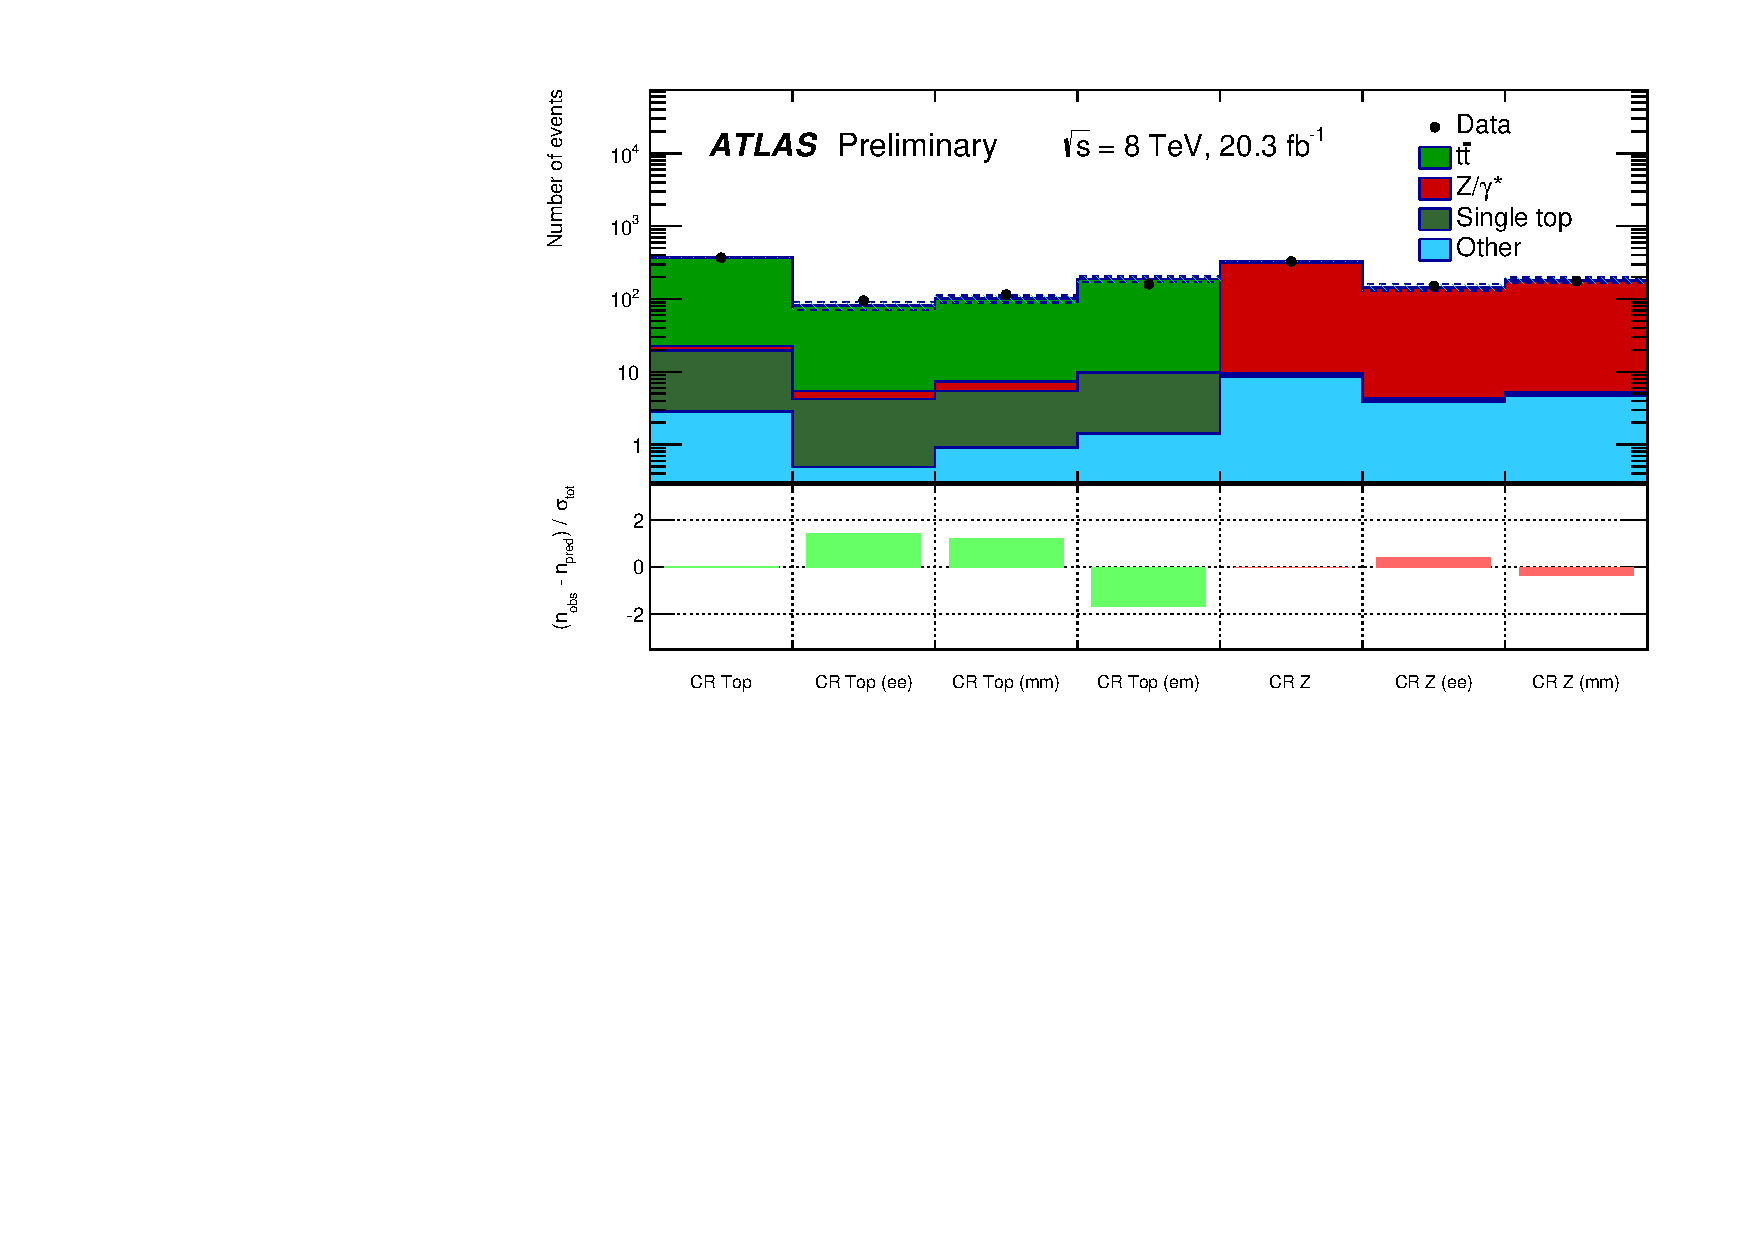
\includegraphics[width=\textwidth]{figs/blstop/histpull_CR_detailed.pdf}
\caption{The top of this plot shows the number of observed and expected
  events in the CRs, and broken down by flavor channel.
  The uncertainty band includes the statistical uncertainty as well as the
  systematic uncertainty (described in Section~\ref{sec:systematics}). The
  bottom of the plot shows the deviation of that channel's prediction
  from the observed number of events divided by the uncertainty on the
  prediction. The normalization of the background yields are determined
  by fitting the \TTBAR\ and \ZGAMMAJETS\ backgrounds to the observed
  data in the two CRs, so the Top CR and $Z$ CR bins have perfect agreement by
  construction.
}
\label{fig:pull_dist_cr}
\end{figure}

\begin{figure}[ht]
\centering
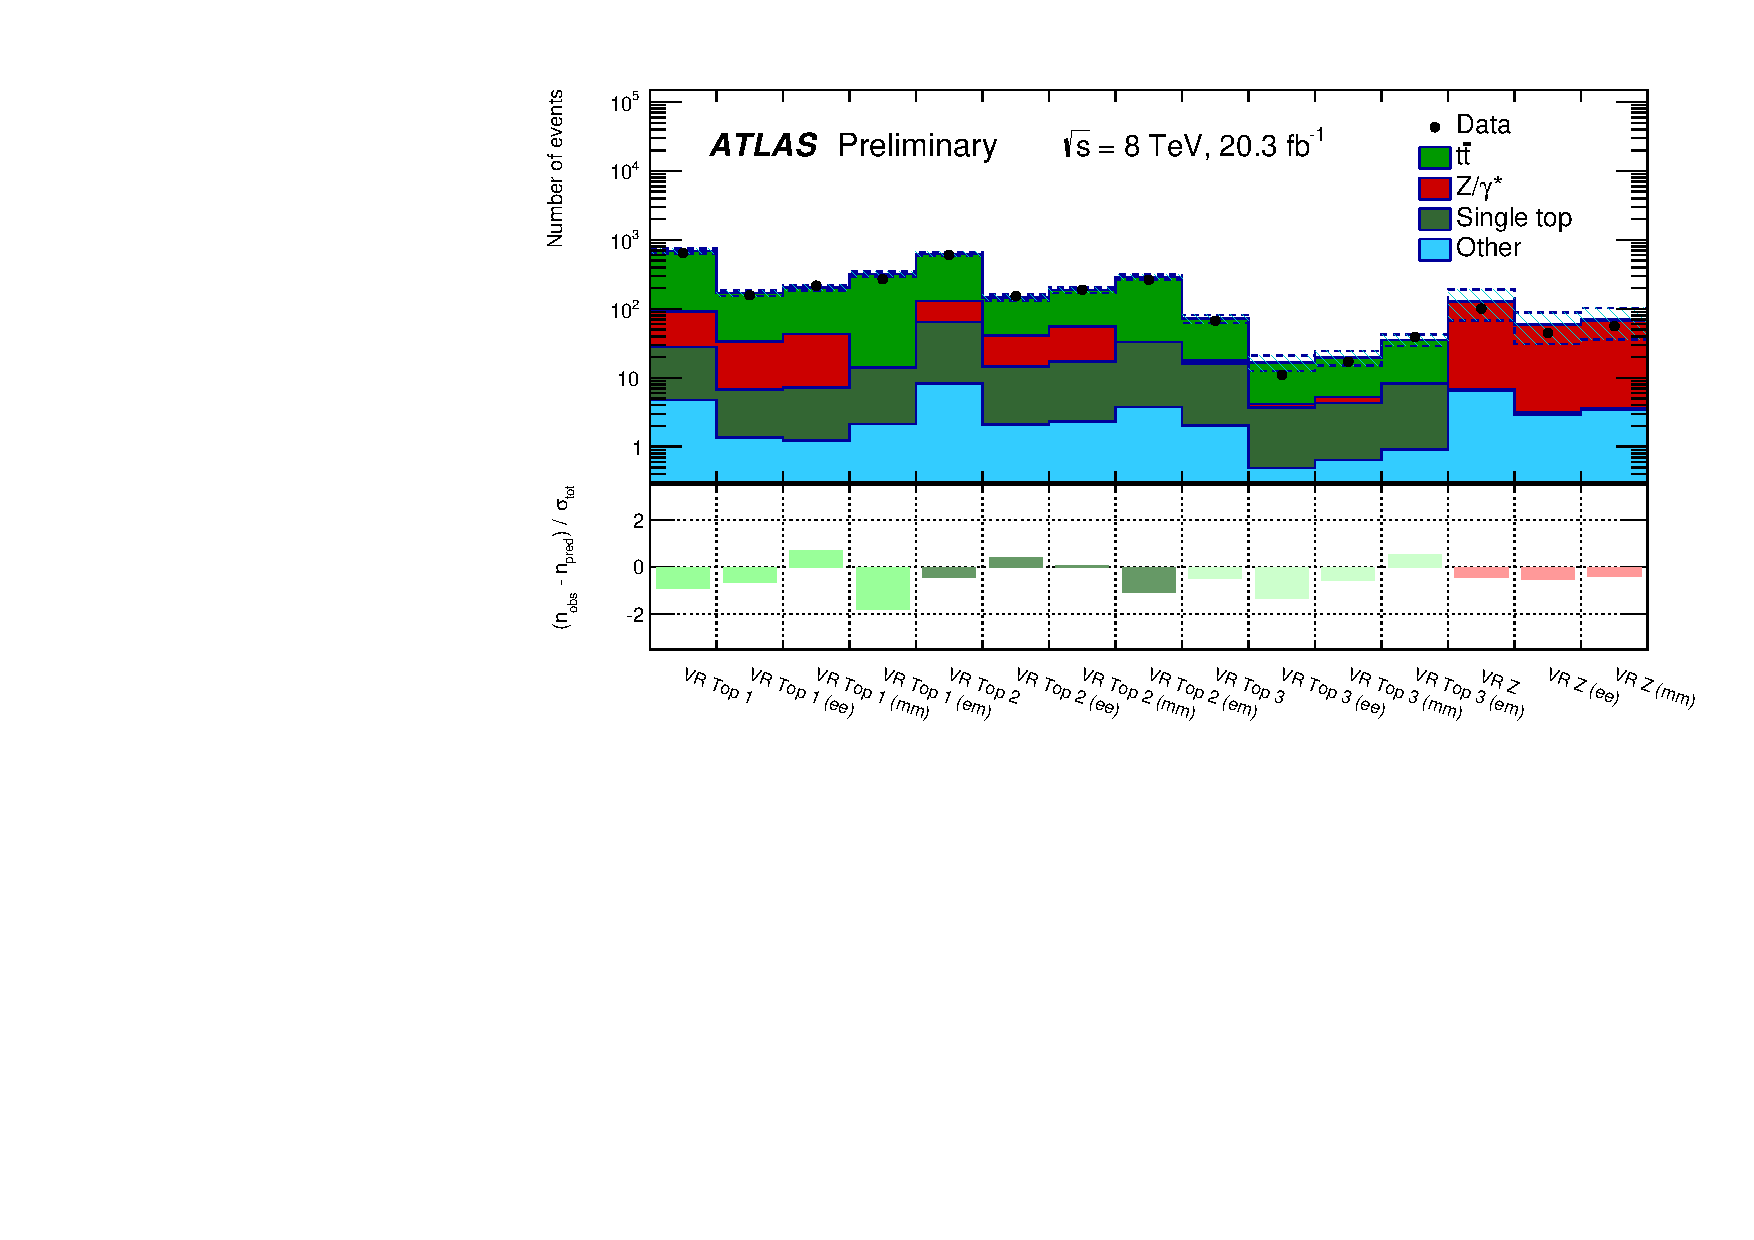
\includegraphics[width=\textwidth]{figs/blstop/histpull_VR_detailed.pdf}
\caption{The top of this plot shows the number of observed and expected
  events in the VR, and broken down by flavor channel.
  The uncertainty band includes the statistical uncertainty as well as the
  systematic uncertainty (described in Section~\ref{sec:systematics}). The
  bottom of the plot shows the deviation of that channel's prediction
  from the observed number of events divided by the uncertainty on the
  prediction. The normalization of the background yields are determined
  by fitting the \TTBAR\ and \ZGAMMAJETS\ backgrounds to the observed
  data in the two CRs.
}
\label{fig:pull_dist_vr}
\end{figure}

The extrapolation from low \HT\ CRs to the high \HT\ region
where the SRs are located is validated using the Top VR 3
and $Z$ VR. These validation regions show fair
agreement between the observed and predicted event yields as well as
for the shape of the $\MBL^{0}$ and \HT\ distributions as shown in
Figures \ref{fig:mbl_vr} and \ref{fig:ht_vr}.

\begin{figure}
  \centering
  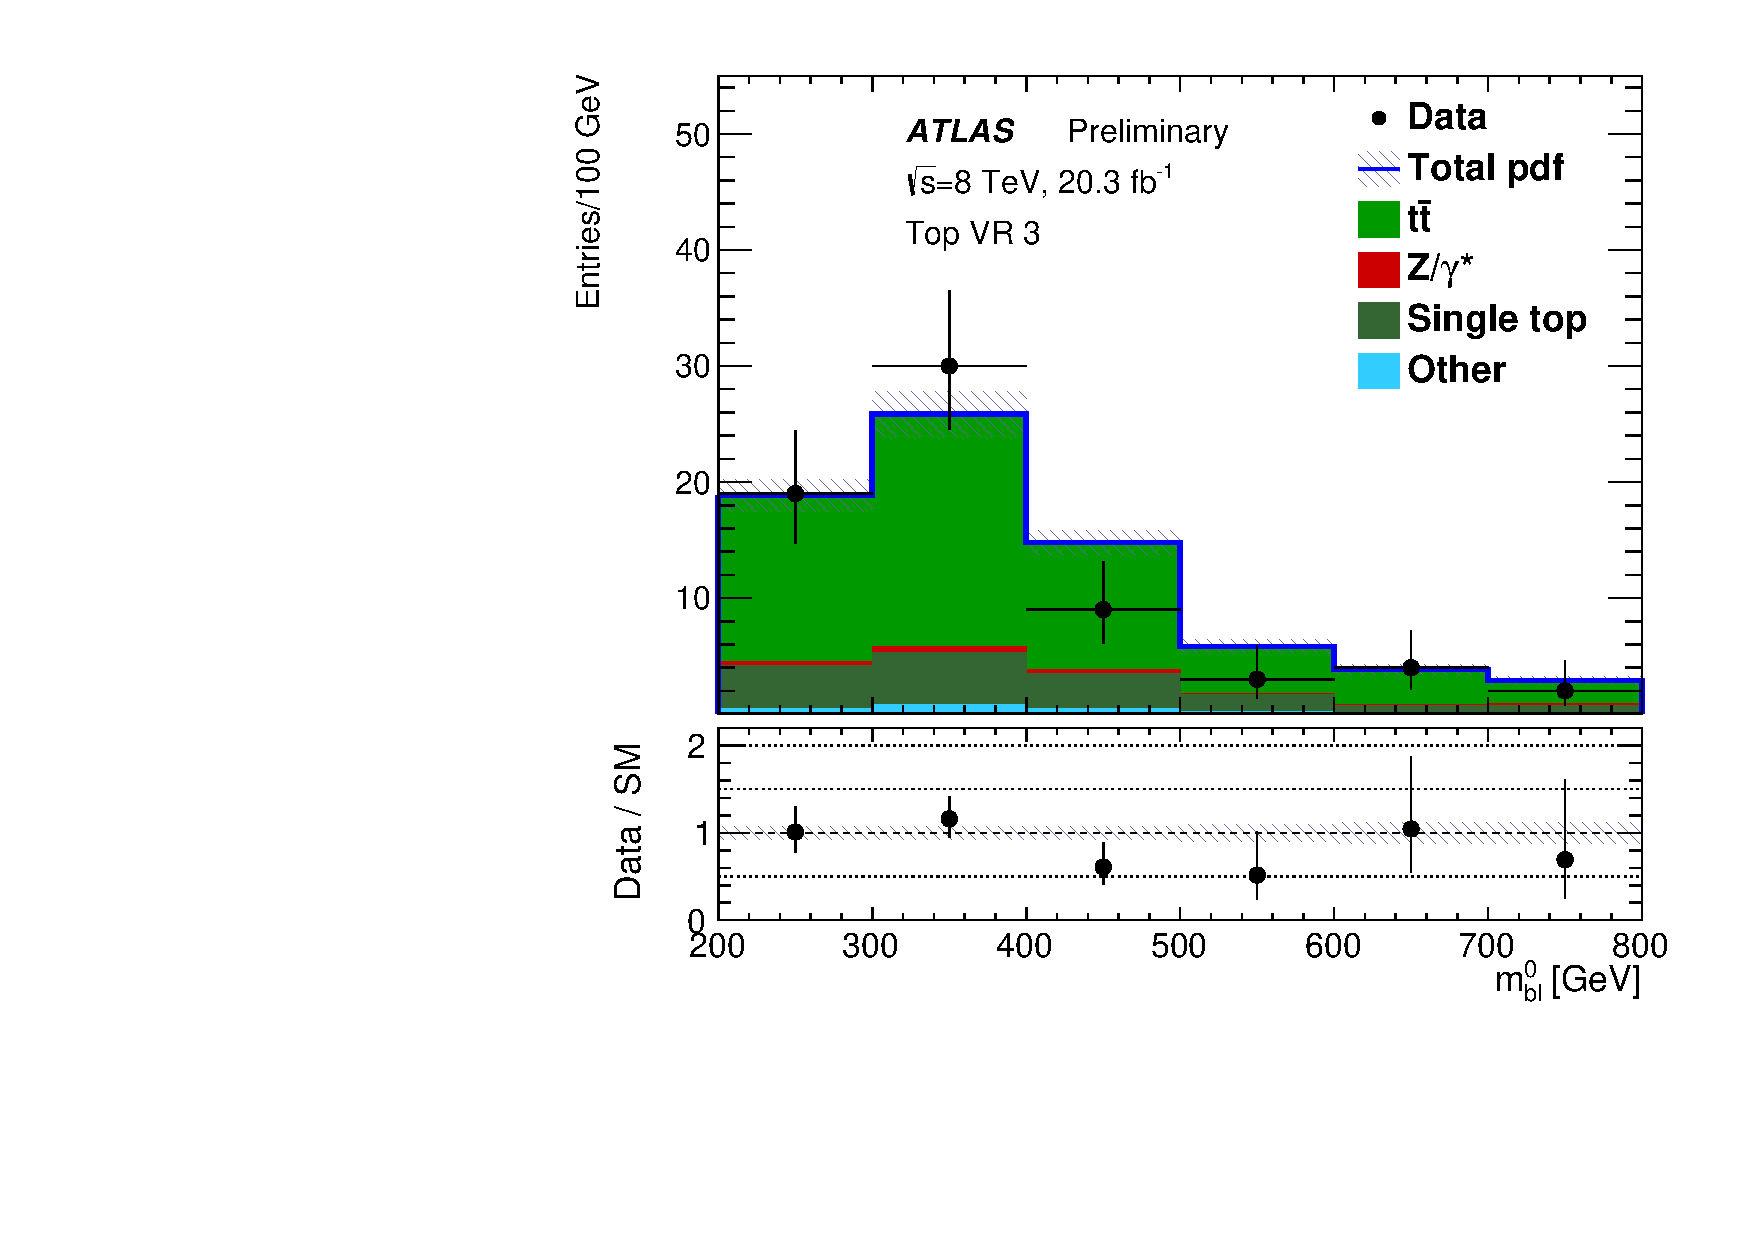
\includegraphics[width=0.48\textwidth]{figs/blstop/vr_top_3_mbl_0.pdf}
  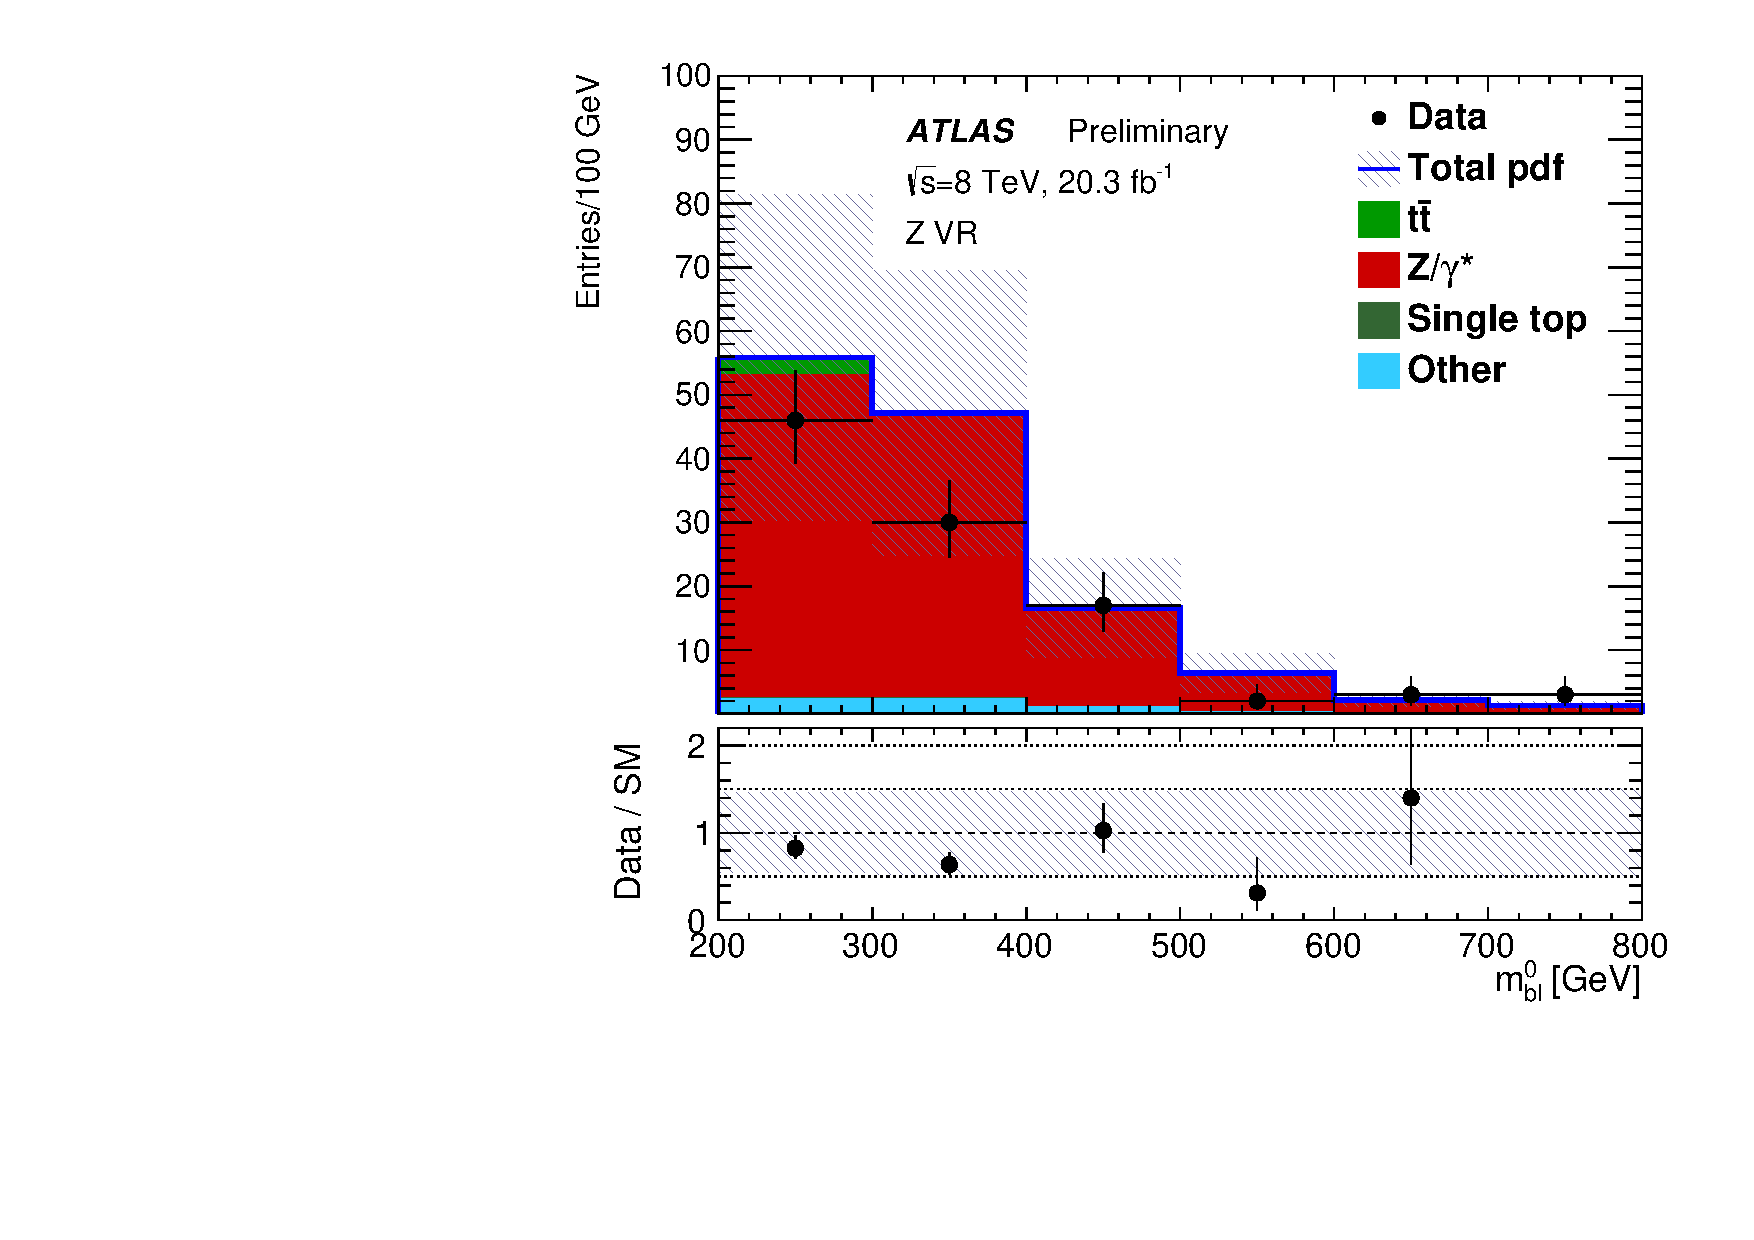
\includegraphics[width=0.48\textwidth]{figs/blstop/vr_Z_mbl_0.pdf}
  \caption{The $\MBL^0$ distribution in Top VR 3 (left) and $Z$ VR (right).
    The Standard Model background prediction is shown after setting the
    normalization of the \TTBAR\ and \ZGAMMAJETS\ backgrounds based on the
    observed data in the CRs. The hashed bands show the uncertainty on the
    fitted background prediction including all statistical and systematics
    uncertainties.
    The bottom of each plot shows the ratio of the observed data to the
    Standard Model background prediction.
  }
  \label{fig:mbl_vr}
\end{figure}

\begin{figure}
  \centering
  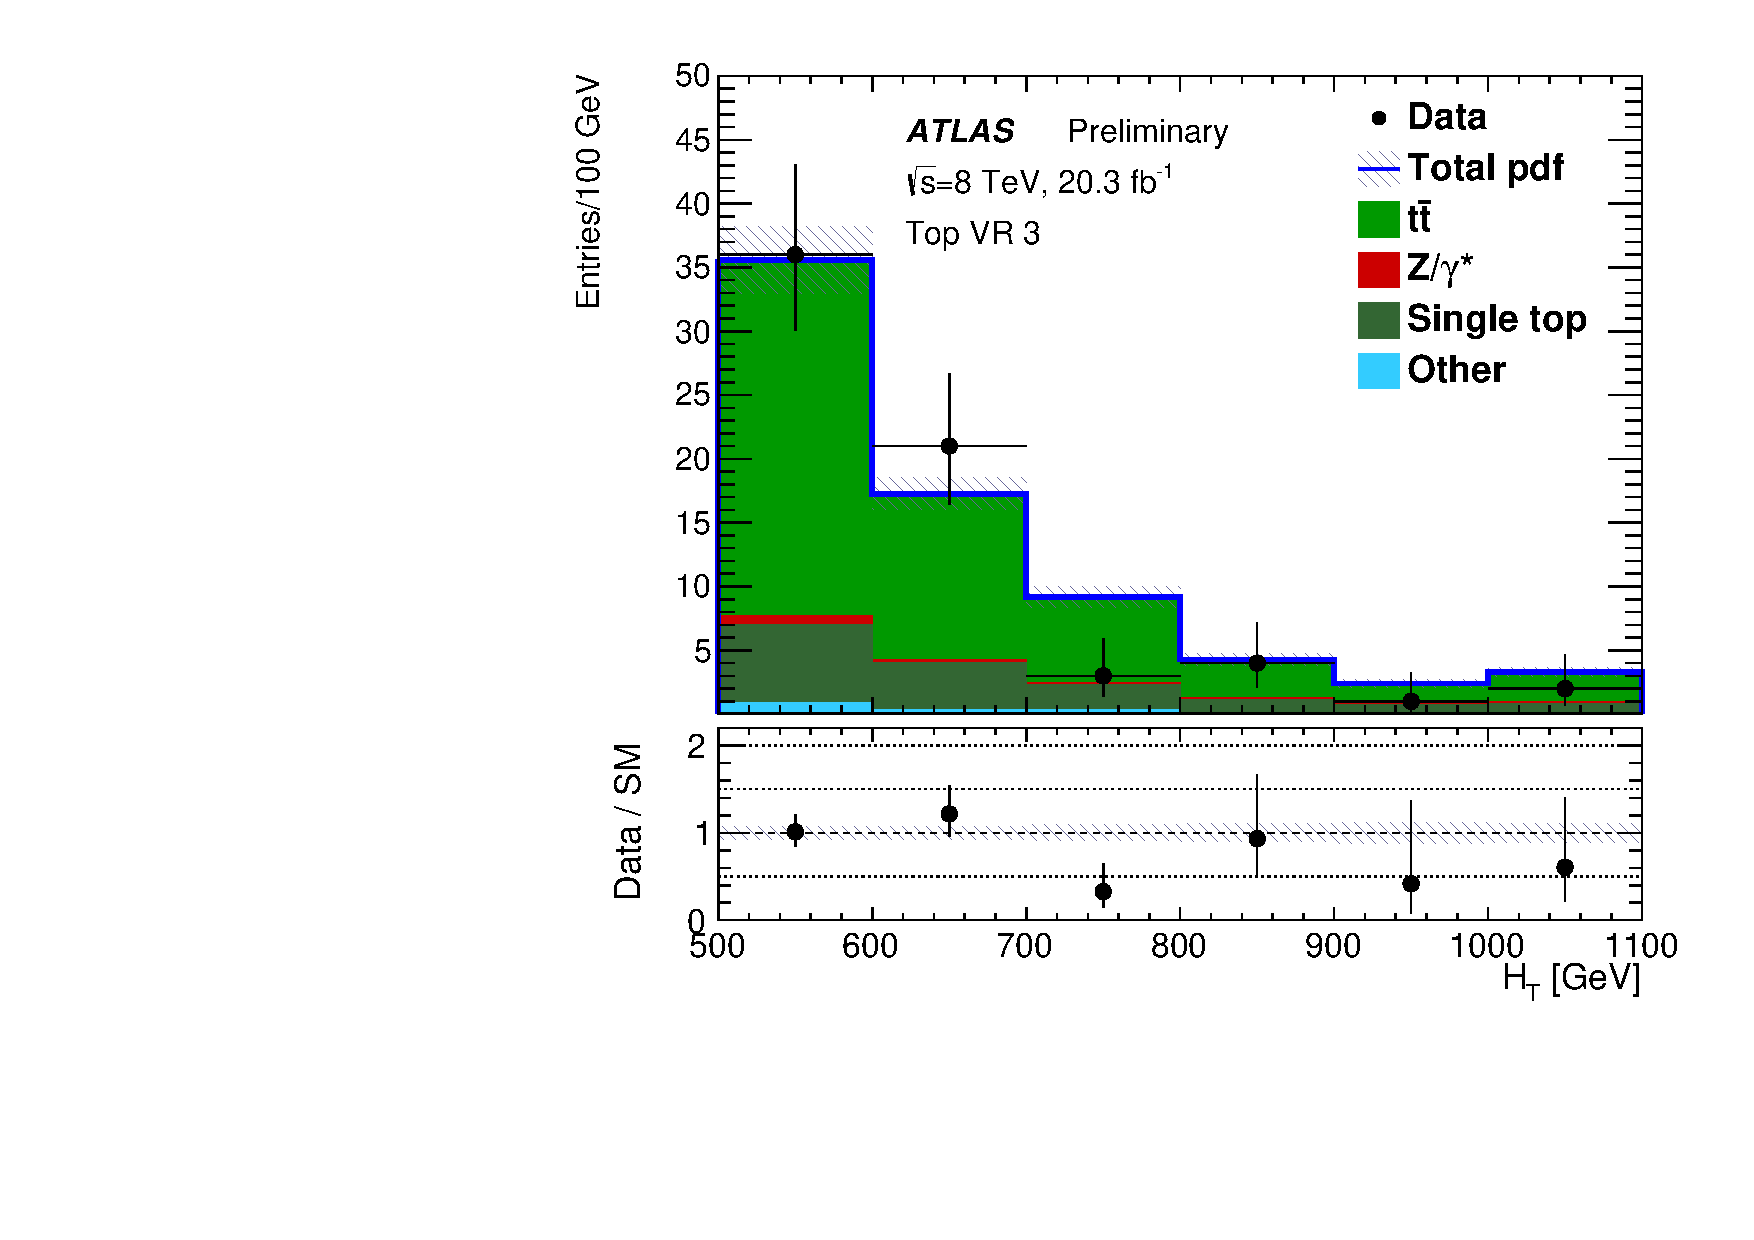
\includegraphics[width=0.48\textwidth]{figs/blstop/vr_top_3_ht_signal.pdf}
  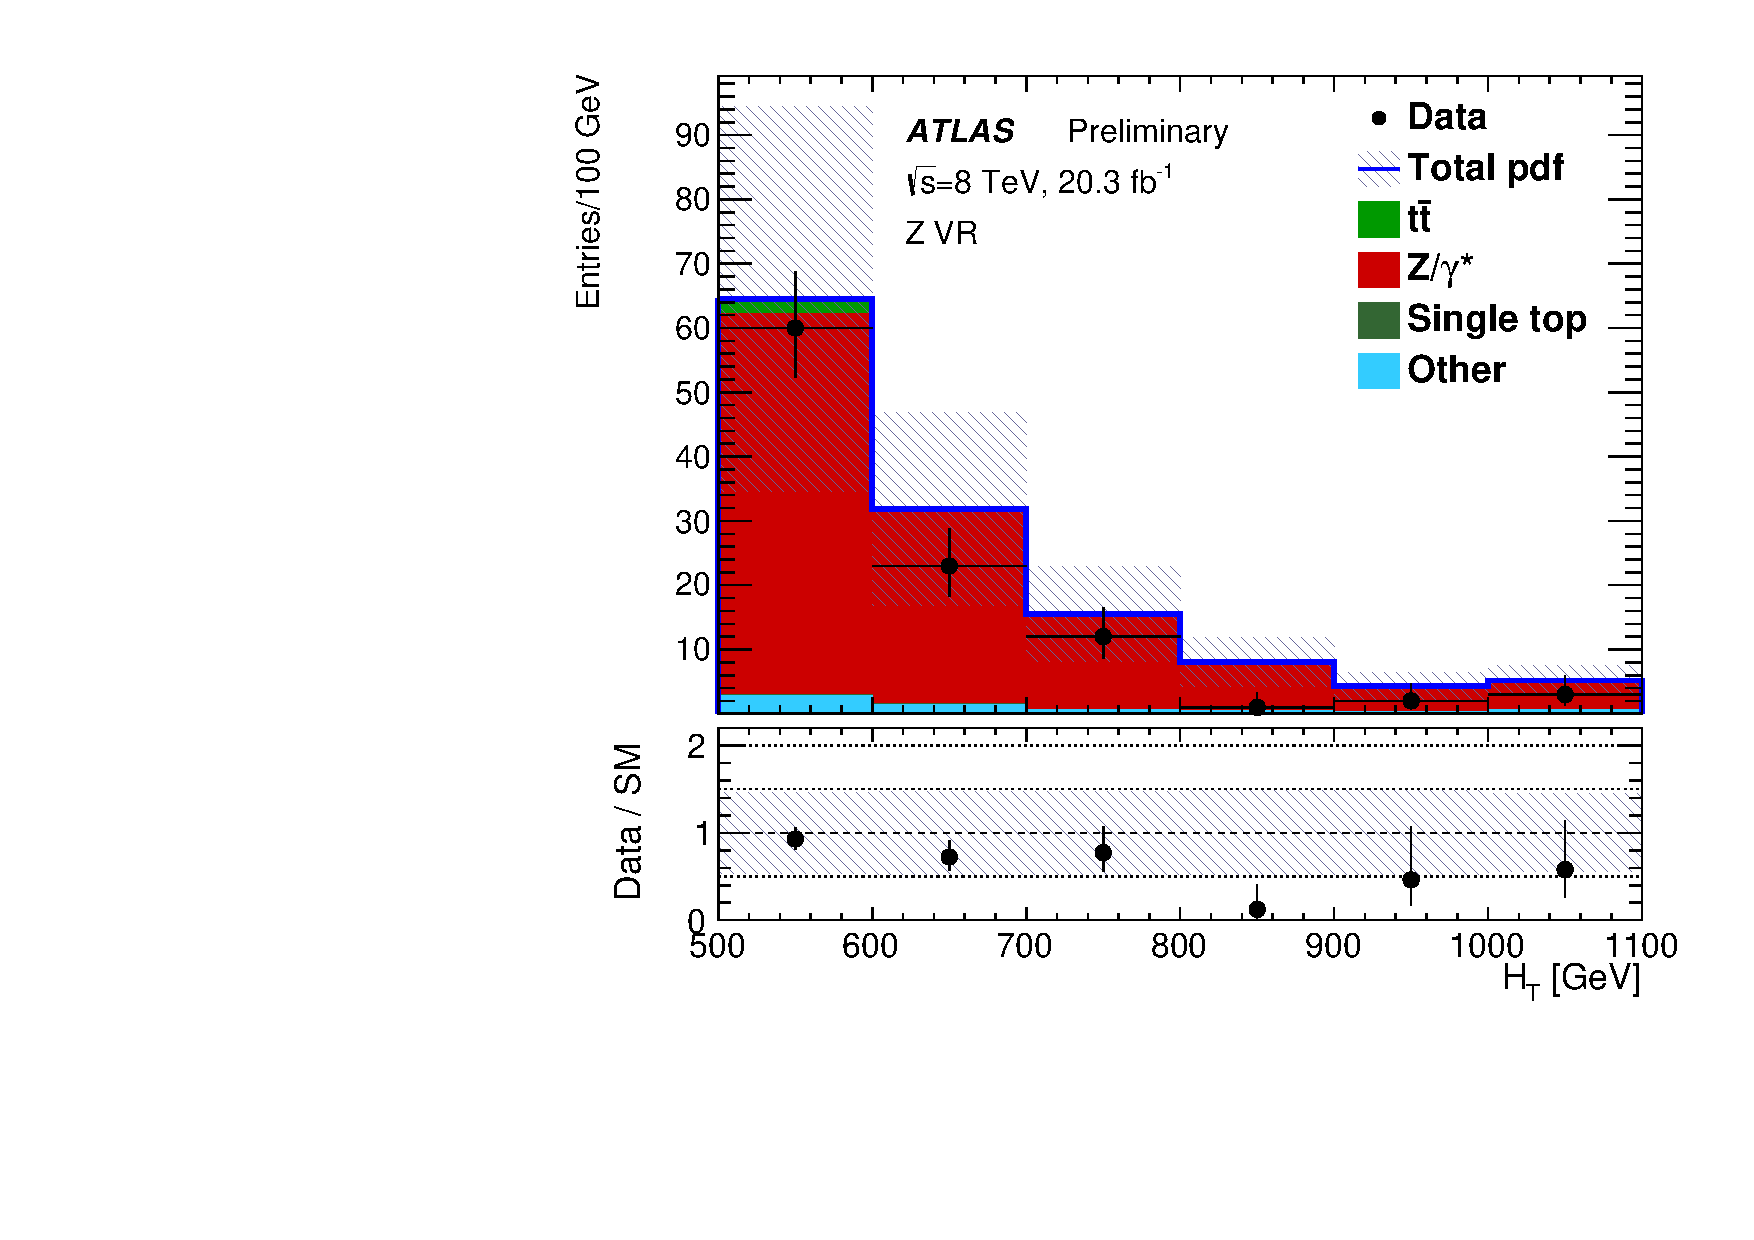
\includegraphics[width=0.48\textwidth]{figs/blstop/vr_Z_ht_signal.pdf}
  \caption{The \HT\ distribution in Top VR 3 (left) and $Z$ VR (right).
    The Standard Model background prediction is shown after setting the
    normalization of the \TTBAR\ and \ZGAMMAJETS\ backgrounds based on the
    observed data in the CRs.
    The hashed bands show the uncertainty on the fitted background prediction
    including all statistical and systematics uncertainties.
    The bottom of each plot shows the ratio of the observed data to the
    Standard Model background prediction.
  }
  \label{fig:ht_vr}
\end{figure}


%% -----------------------------------------------------------------------------
\section{Systematic uncertainties}
\label{sec:systematics}

In addition to the statistical uncertainty, several sources of systematic
uncertainty are considered when determining the estimated signal and background
contributions.
The largest sources of systematic uncertainty are those related to the
MC statistical uncertainty in the SRs, the JES, the $b$-tagging efficiency
The uncertainty on the lepton energy scale and resolution was considered,
but shown to be negligible.

%% - - - - - - - - - - - - - - - - - - - - - - - - - - - - - - - - - - - - - - -
The uncertainty on the jet energy scale (JES) has an impact on both the jet
selection criteria and the kinematics of the event, such as the \HT\ and the
\MET\ measurements.
The JES uncertainty is evaluated using the EM+JES scheme as described
in~\cite{JES}, and the scaling is provided by the
\texttt{MultijetJESUncertaintyProvider} tool.
The uncertainty on the JES is composed of 16 parameters, and takes into account
the dependence on \pt, $\eta$, jet flavor, and the number of primary vertices.
The effect of each component on the event yield is estimated by varying the
component by $\pm 1 \sigma$ in the MC simulation and re-running the full event
selection, propagating the variation in the JES to the jet selection and related
kinematic quantities.

%% - - - - - - - - - - - - - - - - - - - - - - - - - - - - - - - - - - - - - - -
The uncertainty on the jet energy resolution (JER) is evaluated by applying an
additional smearing to the \pt\ measurement of each of the jets in the MC
simulation.
The size of the smearing is determined in dijet events as described
in~\cite{JER}.
The smearing is provided by the \texttt{JetSmearingTool} tool, and depends on
the \pt\ and \eta\ of the jets within an event.
The JER smearing alters the \pt\ of the jets within the event, and therefore
the event selection.
As with the JES, the JER uncertainty is evaluated by re-running the full event
selection on MC simulation, applying the smearing, then propagating the
variations to the event kinematic variables and yields.

%% - - - - - - - - - - - - - - - - - - - - - - - - - - - - - - - - - - - - - - -
As flavor tagging is used in this analysis, the efficiency of the $b$-tagging
algorithms affects the overall yields in each of the analysis regions.
This includes the possibility of a light flavor jet being incorrectly tagged
as a $b$-jet, or a jet which initiated by a $b$-quark failing the $b$-tagging
requirement.
The $b$-tagging efficiency uncertainty is broken into three components,
corresponding to the tagging and rejection efficiency of the different jet
flavors, $b$-jets, $c$-jets, and light flavor jets (light quarks and gluons).
These uncertainties take into account the dependence on \pt\ and jet flavor.
For the MC simulation, the $b$-tagging efficiency is implemented as a scale
factor, so the $b$-tagging uncertainty can be evaluated without running the
full event selection multiple times.
Rather, the $b$-tagging scale factor is varied up or down based on the specific
parameter of interest, and used to determine the uncertainty on the event yield.

%% - - - - - - - - - - - - - - - - - - - - - - - - - - - - - - - - - - - - - - -
The backgrounds are constrained in the CRs which are regions with low \HT,
while the SRs require high \HT.
Top VR 3 and $Z$ VR are used to assess any uncertainty associated with the
extrapolation from low \HT\ to high \HT.
The \TTBAR\ background extrapolation is assessed using Top VR 3. It can be seen
from Table \ref{tab:bkg_only_fit_results} that the post-fit background estimate
in Top VR 3 is in reasonably agreement with the observed data, so no additional
uncertainty is applied to the \TTBAR\ backgrounds due to the \HT\ extrapolation.
The \ZGAMMAJETS\ background extrapolation is assessed using the $Z$ VR.
The overall background is overpredicted in this region by 29\%, and the
prediction is the worst in the highest \HT\ bins.
An additional uncertainty of 50\% is applied to the \ZGAMMAJETS\ background
for events with $\HT > 500 GeV$.
% An \HT\ extrapolation uncertainty of 50\% is applied to \ZGAMMAJETS\ events
% with $\HT \geq 500$~\GeV. This is assigned to account for uncertainty on
% the \ZGAMMAJETS\ \HT\ spectrum. This uncertainty is derived from the
% disagreement observed in Figures~\ref{fig:pull_dist_vr}-\ref{fig:ht_vr}.
%%

%% - - - - - - - - - - - - - - - - - - - - - - - - - - - - - - - - - - - - - - -
Several theoretical uncertainties are considered in the modeling of the major
background processes in MC simulation.
These include the uncertainty on the cross sections, scale variations, and
generator uncertainties.
These uncertainties are evaluated by performing the event selection using only
the MC truth information, and comparing the expected event yields obtained
from MC simulation samples produced using different generator configurations.
An additional systematic uncertainty, due to the $\pm 2.8$\% uncertainty on the
integrated luminosity is evaluated for all background processes except
\TTBAR\ and \ZGAMMAJETS, because these backgrounds take the normalization from
data control regions.
A breakdown of the estimated effect of each source of systematic uncertainty
(both experimental and theoretical) are outlined in
Table~\ref{tab:systematic_breakdown}.

%% - - - - - - - - - - - - - - - - - - - - - - - - - - - - - - - - - - - - - - -
%% ttbar theory systematics
The sources of systematic uncertainty specific to the \TTBAR\ background include
the renormalization and factorization scale variations, MC generator
uncertainties, parton shower, and the amount of initial or final state
radiation (ISR or FSR) in the event.
%%
% scale variations
The scale variations are evaluated by comparing the expected event yields at the
truth level obtained using dedicated \TTBAR\ samples, each generated using
\powheg\ and \pythia, where the factorization and renormalization
scales are varied up and down by a factor of 2.
This isolates the effect of each of the scale variations, and the difference in
expected number of events in each region is taken to be the uncertainty on the
\TTBAR\ background.
The differences in the expected event yields for these samples is take to be
the uncertainty due to the scale variations.
%%
% MC generator
The MC generator uncertainty accounts for the difference in the MC predictions
obtained using different generator programs.
These are assessed by comparing the truth level event selection for a
\TTBAR\ sample generated using \powheg\ and \jimmy\ with a sample
generated using \mcnlo\ and \jimmy.
Since \jimmy\ is used to perform the parton shower in both of these
samples, the differences can be attributed to the differences in the
generation rather than the parton shower step.

%%
% parton shower
The uncertainty in the parton shower in \TTBAR\ samples is estimated by
comparing the expected event yields using the truth level information for two
\TTBAR\ samples each generated using \powheg.
One sample uses \pythia\ for the parton shower step, while the other
uses \jimmy.
This isolates the parton shower part of the MC simulation, which is performed
either using \pythia\ or \jimmy.
%%
% ISR/FSR
The uncertainty on the ISR and FSR is evaluated by comparing the expected number
of events in a truth level event selection found in two \TTBAR\ samples, each
generated using \acermc\ and \pythia.
The two samples differ in the amount of parton shower is included in the
simulation.
%%

%% - - - - - - - - - - - - - - - - - - - - - - - - - - - - - - - - - - - - - - -
%% single top theory systematics
The sources of systematic uncertainty specific to the single top background
include the single top cross section, the MC generator uncertainties, the parton
shower, ISR and FSR, and the interference with \TTBAR.
%%
% cross section
Single top can be produced through three production channels, with production
cross sections
\begin{itemize}
  \item $s$-channel: $5.61 \pm 0.22$ pb
  \item $t$-channel: $87.76^{+3.44}_{-1.91}$ pb
  \item $Wt$-channel: $22.37 \pm 1.52$ pb.
\end{itemize}
It was shown that the $Wt$-channel is dominant single top production channel for
the regions of interest.
For his reason, the uncertainty on the $Wt$-channel cross section is the only
single top cross section uncertainty which is considered, and a systematic
uncertainty of 7\% was applied to the single top background estimate in every
analysis region.
%%
% MC gen uncertainty.
The MC generator uncertainty on the single top background estimate is evaluated
by comparing the predicted yields from two single top samples, one generated
using \powheg, and the other generated using \mcnlo.
Both MC samples use \herwig\ to calculate the parton shower.
%%
% parton shower
The parton shower uncertainty is determined by comparing the truth level yields
of two simulated $Wt$-channel samples, each generated using \herwig.
The parton shower step was performed using \pythia\ and \herwig.
%%
% ISR/FSR
Similar to the \TTBAR\ background, the uncertainty on the single top background
estimate due to ISR and FSR uncertainties is determined by comparing two
samples, each generated using \acermc\ and \pythia, where the two samples
differ in the amount of parton shower is included in the simulation
%%
% ttbar interference
There is some interference between the \TTBAR\ and the $Wt$-channel single top
background processes.
This interference is handled by applying an additional uncertainty to the single
top background estimate by comparing the truth level event selection of two
$Wt$-channel samples, each generated using \powheg, but one using the DS
renormalization scheme, and the other using the DR renormalization scheme.

%% - - - - - - - - - - - - - - - - - - - - - - - - - - - - - - - - - - - - - - -
%% Z+jets theory systematics
In addition to the \HT\ extrapolation uncertainty discussed previously, an
additional uncertainty is applied to account for the finite number of partons in
the \ZGAMMAJETS\ background MC samples.
This uncertainty is evaluated by comparing the truth level event yields for two
\ZGAMMAJETS\ samples, generated with different numbers of additional partons
included in the matrix element calculation.
The first sample has exactly four additional partons in the matrix element
calculation, while the second set has four or five additional partons.
Both samples are generated using \sherpa.

%% - - - - - - - - - - - - - - - - - - - - - - - - - - - - - - - - - - - - - - -
%% MC stat systematics
In addition to the above sources of systematic uncertainty, the uncertainty
on the background estimate due to limited MC statistics in the CRs and SRs is
considered.
The MC statistical uncertainty was evaluated for each background process
independently in each analysis region as
\begin{equation}
  \sigma_{r,p}^\mathrm{MC~stat}
  =
  \sqrt{N_{r,p}^\mathrm{gen}},
\end{equation}
where $r$ and $p$ represent the region and background MC process respectively.
$N_{r,p}^\mathrm{gen}$ is the number of MC simulated events from background
process $p$ in region $r$.
No weights or scale factors are applied to this number of simulated events.
The total relative uncertainty in a region $r$ due to MC statistical
limitations ($\sigma_{r}^\mathrm{MC~stat,relative}$) is obtained by summing the
relative uncertainties for each process in region $r$ in quadrature, giving
\begin{equation}
  \sigma_{r}^\mathrm{MC~stat,relative}
  =
  \sqrt{ \sum_{p} \left(\frac{\sigma_{r,p}^\mathrm{MC~stat}}{N_{r,p}^\mathrm{gen}}\right)^2 }
  =
  \sqrt{ \sum_{p} \frac{1}{N_{r,p}^\mathrm{gen}} }.
\end{equation}
The total MC statistical uncertainty is evaluated in each region, and treated
as a systematic uncertainty on the background estimate.
The Top CR and $Z$ CR are used to constrain the \TTBAR\ and
\ZGAMMAJETS\ background estimates, so the MC statistical uncertainty in the
CRs results in additional uncertainty on the background estimate in the SRs.
For this reason, the MC statistical uncertainty in the Top ($Z$) CR is applied
as an additional systematic uncertainty on the \TTBAR\ (\ZGAMMAJETS) background
estimate in the SRs.

%% - - - - - - - - - - - - - - - - - - - - - - - - - - - - - - - - - - - - - - -
\begin{table}[ht]
\caption{Summary of the effect of each considered sources of systematic
  uncertainty on the background estimate in SR~400 and SR~600. Several
  sources of theoretical systematic uncertainty which have a small
  effect on the total background estimate are grouped into the
  ``Other theory'' category.
  {\color{red} TODO update this table with broken down info and CRs.}
}
\label{tab:systematic_breakdown}
%
\centering{
  \begin{tabular}{lcc}
  \toprule
    Systematic &
    \multirow{2}{*}{SR~400} &
    \multirow{2}{*}{SR~600} \\
    Uncertainty (\%) \\
    \midrule
    JES                          & 15     & 3  \\
    $b$-tagging                  & 13     & 12 \\
    JER                          & 5      & 1  \\
    Luminosity                   & 1      & 1  \\
    \midrule                                   
    \HT\ extrapolation           & 19     & 20 \\
    MC statistical               & 13     & 23 \\
    CR statistical               & 3      & 3 \\
    $Wt$ cross section           & 2      & 2  \\
    Other theory                 & 1      & 2  \\
    \bottomrule
    \end{tabular}
}
\end{table}

When determining the expected contributions of each of the signal models,
the effects of the JES, $b$-tagging efficiency, JER, and luminosity are
considered as well as the uncertainty on the signal model cross section which
ranges between 14\% and 28\%.

%% -----------------------------------------------------------------------------
\section{Results}
\label{sec:results}

The background yields in these signal regions are determined by a maximum
likelihood fit~\cite{Baak:2014wma} for the \TTBAR\ and
\ZGAMMAJETS\ normalizations, which are constrained by the observed data in the
Top and $Z$ CRs.
The systematic uncertainties described previously are included as
Gaussian-distributed nuisance parameters.
The fitted background yields and the observed number of events in each
signal region are shown in Tables~\ref{tab:event_yields_sr_400} and
\ref{tab:event_yields_sr_600}. Two events are observed, in agreement with
the Standard Model prediction.  The kinematics of the two selected events
are shown in Table~\ref{tab:sr_event_kinematics}, the $\MBL^0$ and
\HT\ distributions in SR 400 are shown in Figure~\ref{fig:sr_dists}.

\begin{table}
  \caption{The expected and observed event yields in SR~400. The expected event
    yields are shown before and after performing the fit to the data in the
    control regions.
    The last three rows show the model-independent 95\% CL on
    the visible cross section and the number of events (expected and observed)
    in SR~400 from a generic non-Standard Model process.
  }
  \label{tab:event_yields_sr_400}
  %
  \begin{center}
    \begin{tabular}{lrrrr}
      \toprule
                                     & SR~400                & SR~400 $ee$           & SR~400 $\mu\mu$       & SR~400 $e\mu$  \\
      \midrule
      Observed                       & $2$                   & $0$                   & $2$                   & $0$                \\
      \midrule
      Fitted background              & $1.39 \pm 0.35$       & $0.36 \pm 0.15$       & $0.57 \pm 0.20$       & $0.45 \pm 0.11$    \\
      \midrule
      Fitted \TTBAR                  & $0.33 \pm 0.09$       & $0.07 \pm 0.08$       & $0.07 \pm 0.02$       & $0.19 \pm 0.05$    \\
      Fitted \ZGAMMAJETS             & $0.54 \pm 0.28$       & $0.20 \pm 0.10$       & $0.35 \pm 0.18$       & $\leq 0.01$    \\
      Single Top                     & $0.44 \pm 0.08$       & $0.10 \pm 0.03$       & $0.11 \pm 0.03$       & $0.23 \pm 0.05$    \\
      Other                          & $0.07 \pm 0.04$       & $\leq 0.01$           & $0.04 \pm 0.02$       & $0.03 \pm 0.03$    \\
      \midrule
      Input SM                       & $1.2$                 & $0.30$                & $0.46$                & $0.43$             \\
      \midrule
      Input \TTBAR                   & $0.30$                & $0.06$                & $0.06$                & $0.17$             \\
      Input \ZGAMMAJETS              & $0.38$                & $0.14$                & $0.24$                & $0.00$             \\
      Input single Top               & $0.44$                & $0.10$                & $0.11$                & $0.23$             \\
      Input other                    & $0.07$                & $0.00$                & $0.04$                & $0.03$             \\
      \midrule
      $\sigma_\mathrm{vis}$~[fb]     & $0.23$                & $0.11$                & $0.26$                & $0.11$                \\
      Observed $N_\mathrm{non-SM}$   & $4.8$                 & $2.2$                 & $5.4$                 & $2.3$                 \\
      Expected $N_\mathrm{non-SM}$   & ${4.0}^{+2.2}_{-1.1}$ & ${3.2}^{+1.7}_{-1.1}$ & ${3.6}^{+1.9}_{-1.5}$ & ${3.3}^{+1.8}_{-1.3}$ \\
      \bottomrule
    \end{tabular}
  \end{center}
\end{table}

\begin{table}
  \caption{The expected and observed event yields in SR~600. The expected event
    yields are shown before and after performing the fit to the data in the
    control regions.  The last three rows show the model-independent 95\% CL on
    the visible cross section and the number of events (expected and observed)
    in SR~600 from a generic non-Standard Model process.
  }
  \label{tab:event_yields_sr_600}
  %
  \begin{center}
    \begin{tabular}{lrrrr}
      \toprule
                                      & SR~600                & SR~600 $ee$           & SR~600 $\mu\mu$       & SR~600 $e\mu$   \\
      \midrule
      Observed                        & $1$                   & $0$                   & $1$                   & $0$              \\
      \midrule
      Fitted background               & $0.55 \pm 0.15$       & $0.15 \pm 0.06$       & $0.24 \pm 0.10$       & $0.16 \pm 0.06$  \\
      \midrule
      Fitted \TTBAR                   & $0.10 \pm 0.02$       & $0.03 \pm 0.01$       & $\leq 0.01$           & $0.07 \pm 0.03$  \\
      Fitted \ZGAMMAJETS              & $0.23 \pm 0.12$       & $0.08 \pm 0.05$       & $0.15 \pm 0.08$       & $\leq 0.01$  \\
      Single Top                      & $0.18 \pm 0.04$       & $0.03 \pm 0.01$       & $0.05 \pm 0.02$       & $0.09 \pm 0.03$  \\
      Other                           & $0.04 \pm 0.01$       & $\leq 0.01$           & $0.04 \pm 0.02$       & $\leq 0.01$  \\
      \midrule
      Input SM                        & $0.47$                & $0.12$                & $0.20$                & $0.16$           \\
      \midrule
      Input \TTBAR                    & $0.09$                & $0.03$                & $0.00$                & $0.06$           \\
      Input \ZGAMMAJETS               & $0.16$                & $0.06$                & $0.10$                & $0.00$           \\
      Input single Top                & $0.18$                & $0.03$                & $0.05$                & $0.09$           \\
      Input other                     & $0.04$                & $0.00$                & $0.04$                & $0.00$           \\
      \midrule
      $\sigma_\mathrm{vis}$~[fb]      & $0.19$                & $0.10$                & $0.20$                & $0.10$                \\
      Observed $N_\mathrm{non-SM}$    & $3.9$                 & $2.1$                 & $4.0$                 & $2.1$                 \\
      Expected $N_\mathrm{non-SM}$    & ${3.5}^{+1.9}_{-1.4}$ & ${2.6}^{+1.6}_{-0.6}$ & ${3.0}^{+1.7}_{-1.0}$ & ${2.7}^{+1.6}_{-0.7}$ \\
      \bottomrule
    \end{tabular}
  \end{center}
\end{table}

\begin{table}
  \caption{The event and object kinematics for the two events passing the
    signal region selection. The first event passes the SR~400 selection
    while the second event passes both SR~400 and SR~600 selections.
  }
  \label{tab:sr_event_kinematics}
  %
  \begin{center}
    \begin{tabular}{lcc}
      \toprule
      Run number              & 214216    & 210302  \\
      Event number            & 121272046 & 2292645861 \\
      \midrule
      $\MBL^0$ [\GeV]         & 558       & 686   \\
      %
      $\ell_0$ flavor         & $\mu$     & $\mu$ \\
      $\ell_0$ charge         & $-$       & $-$   \\
      %
      $\ell_0\ \pt$ [\GeV]    & 375       & 272   \\
      $b_0\ \pt$ [\GeV]       & 330       & 460   \\
      %
      $\ell_0\ \eta$          & $-0.11$   & 1.22  \\
      $b_0\ \eta$             & 0.56      & 0.95  \\
      %
      $\ell_0\ \phi$          & 2.0       & $-1.3$  \\
      $b_0\ \phi$             & $-2.7$    & 2.5   \\
      %
      \midrule
      $\MBL^1$ [\GeV]         & 526       & 528   \\
      %
      $\ell_1$ flavor         & $\mu$     & $\mu$ \\
      $\ell_1$ charge         & $+$       & $+$     \\
      %
      $\ell_1\ \pt$ [\GeV]    & 88        & 96    \\
      $b_1\ \pt$ [\GeV]       & 542       & 374   \\
      %
      $\ell_1\ \eta$          & 0.45      & 1.43  \\
      $b_1\ \eta$             & $-1.1$    & $-0.26$ \\
      %
      $\ell_1\ \phi$          & $-2.3$    & $-0.91$ \\
      $b_1\ \phi$             & $-0.21$   & 2.3   \\
      %
      \midrule
      \MBLASYM                & 0.03      & 0.13  \\
      \HT\ [\GeV]             & 1335      & 1203  \\
      \METSIG\ $[\GeV^{1/2}]$ & 2.9       & 6.4   \\
      \MET\ [\GeV]            & 107       & 223   \\
      $m_{\ell\ell}$ [\GeV]   & 324       & 71    \\
      \bottomrule
    \end{tabular}
  \end{center}
\end{table}

\begin{figure}[ht]
  \centering
  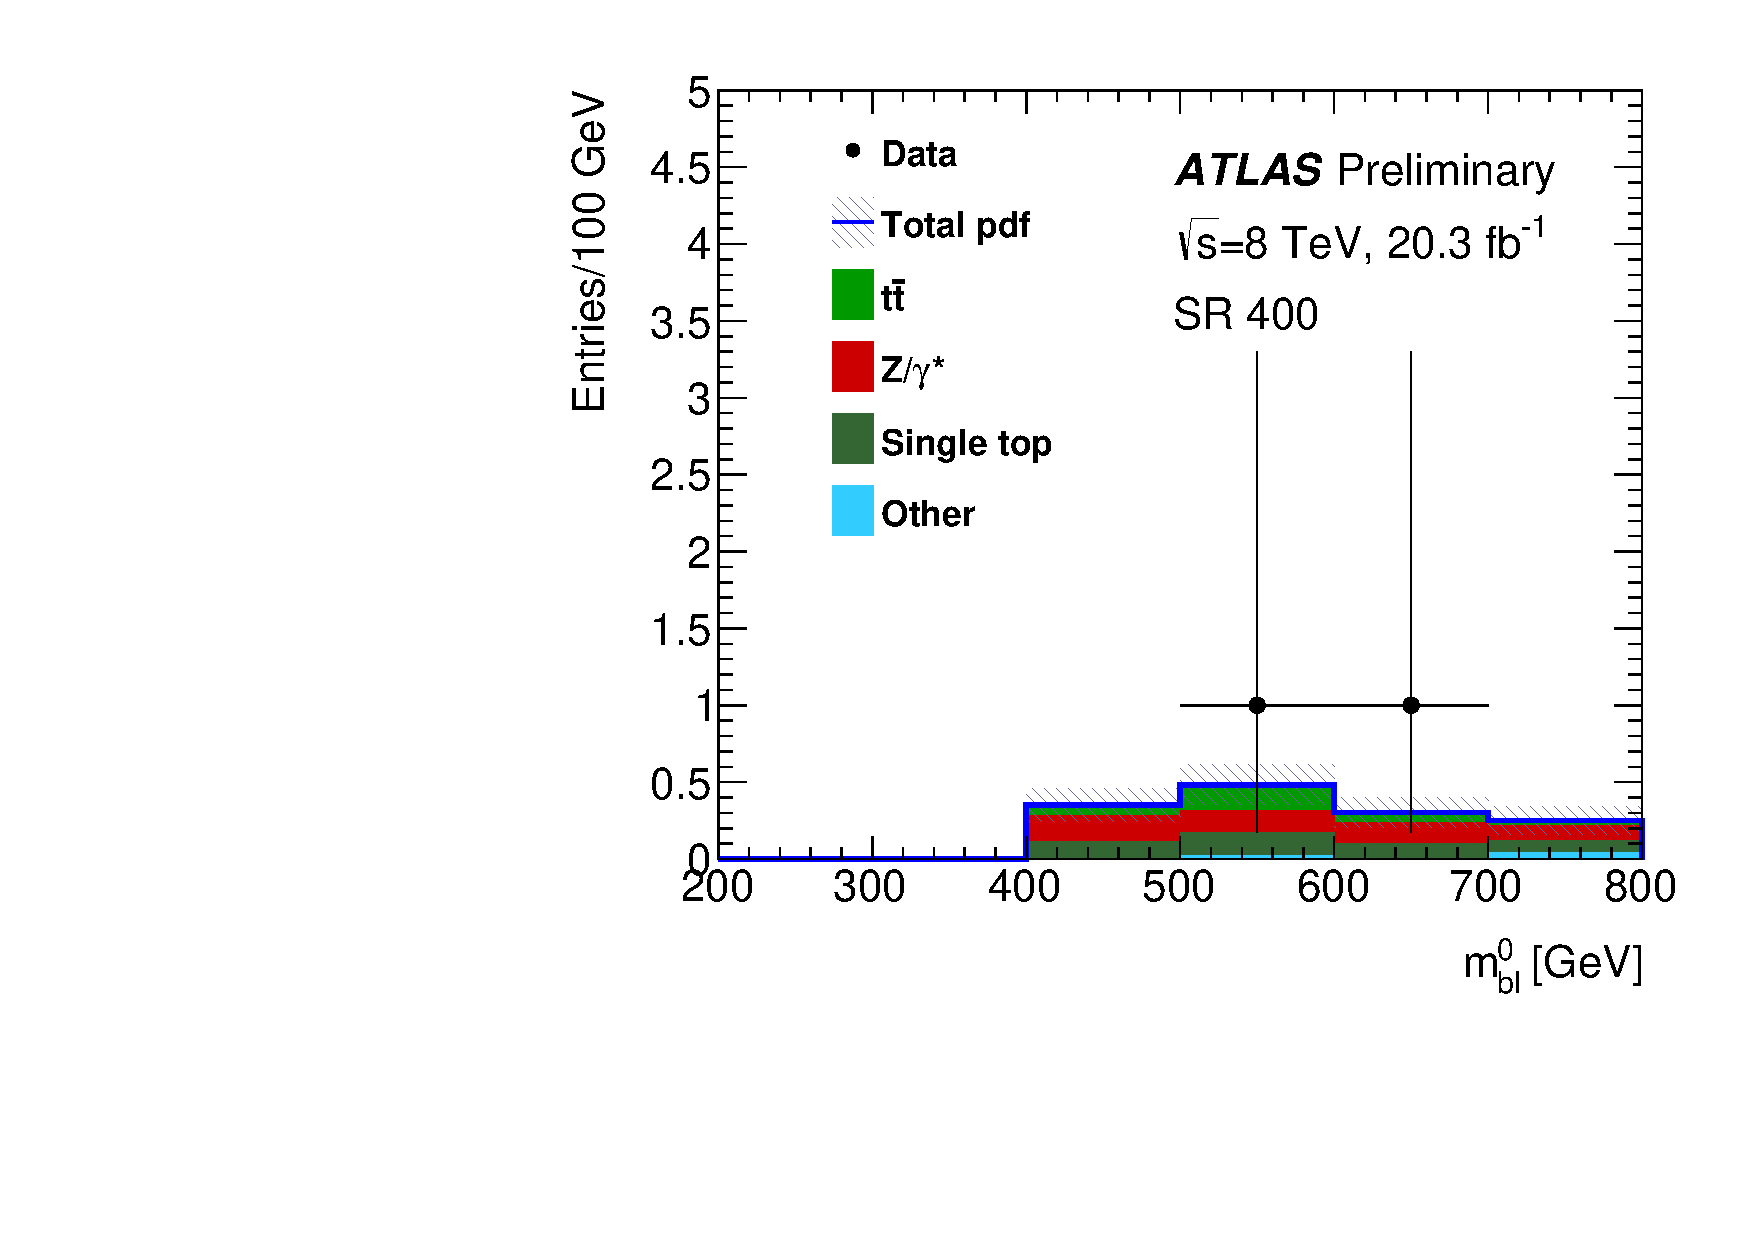
\includegraphics[width=0.45\textwidth]{figs/blstop/sr_mbl_0.pdf}
  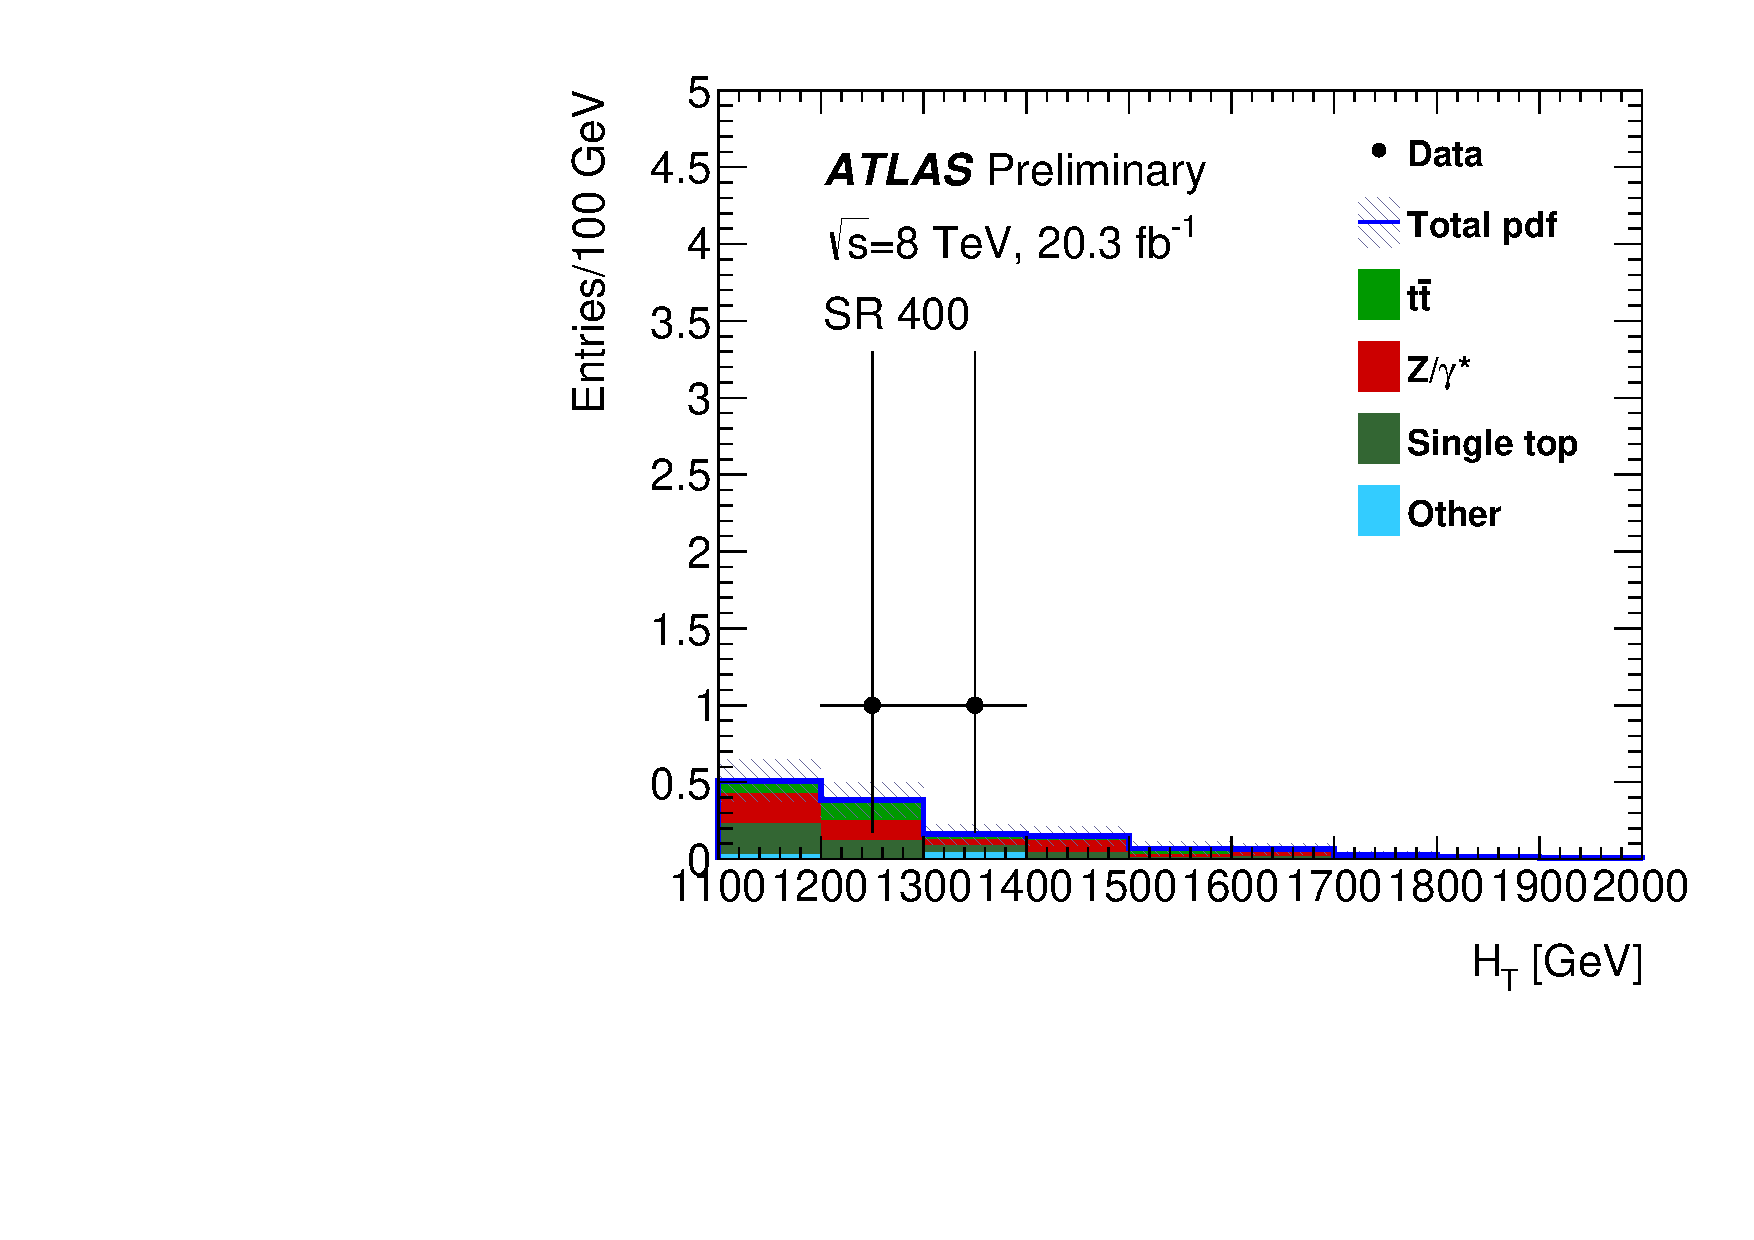
\includegraphics[width=0.45\textwidth]{figs/blstop/sr_ht.pdf}
  \caption{These plots show the $\MBL^0$ (left) and \HT\ (right) distributions
    in SR 400. The Standard Model background prediction is taken from the
    fitted background prediction. The hashed bands show
    the uncertainty on the fitted background prediction including the MC
    statistical and sources of systematic uncertainty.  The bottom of
    each plot shows the ratio of the observed data to the Standard Model
    background prediction.
  }
  \label{fig:sr_dists}
\end{figure}

As the observed number of events is consistent with the Standard Model
prediction, Upper limits at 95\% confidence level (CL) on the number of
beyond the Standard Model (BSM) events for each signal region are derived
using the $CL_s$ prescription and neglecting any possible contamination in the
control regions. Normalizing these by the integrated luminosity of the data
sample they can be interpreted as upper limits on the visible BSM
cross section, $\sigma_\mathrm{vis}$, where $\sigma_\mathrm{vis}$ is defined
as the product of acceptance, reconstruction efficiency and production
cross section. The results are given in
Tables~\ref{tab:event_yields_sr_400}~and~\ref{tab:event_yields_sr_600}.

Exclusion limits on the signal model are determined using the $CL_S$
prescription based on a simultaneous fit of the SRs and
CRs~\cite{Baak:2014wma}. The predicted signal contamination is
taken into account in the CRs.  For each stop mass,
exclusion fits are performed with various assumptions on the branching
ratios of the stop. For each point on the branching ratio plane, the
SR which provided the best expected sensitivity, as
measured by the lowest expected $CL_S$ value, is chosen. The expected
and observed limits are shown in Figure \ref{fig:limit_contours}. This figure
shows, for each simulated stop mass, the observed (expected) 95\% exclusion
limit on the 
branching fraction under the red (blue) line. A yellow band shows the
$\pm 1\sigma$ uncertainty on the expected limit, determined from the
systematic uncertainty on the signal and background prediction excluding
the effect of the signal cross section uncertainty.  The effect of varying
the signal cross section on the observed limit is indicated by the dashed
red lines.  The final limit on the stop mass is shown in
Figure~\ref{fig:mass_limit_obs}.  This plot shows the 95\% confidence
limit~(CL)
on the mass obtained by choosing the maximum excluded mass for each
branching ratio on the plane using the nominal cross section value.  
As the branching ratio of $\tilde{t} \rightarrow b\tau$ increases, the number
of expected events with electrons or muons in the final state decreases
for the same simulated stop mass. Therefore, the limit on the mass is
strongest at the bottom of the plane. In the top corner of the plot, the
SRs described in this analysis note have no sensitivity, however traditional
lepto-quark searches for final states with $b$-tagged jets and $\tau$ leptons
are able to place experimental limits in this region \cite{ATLAS:2013oea}.

\begin{figure}[ht]
  \centering
  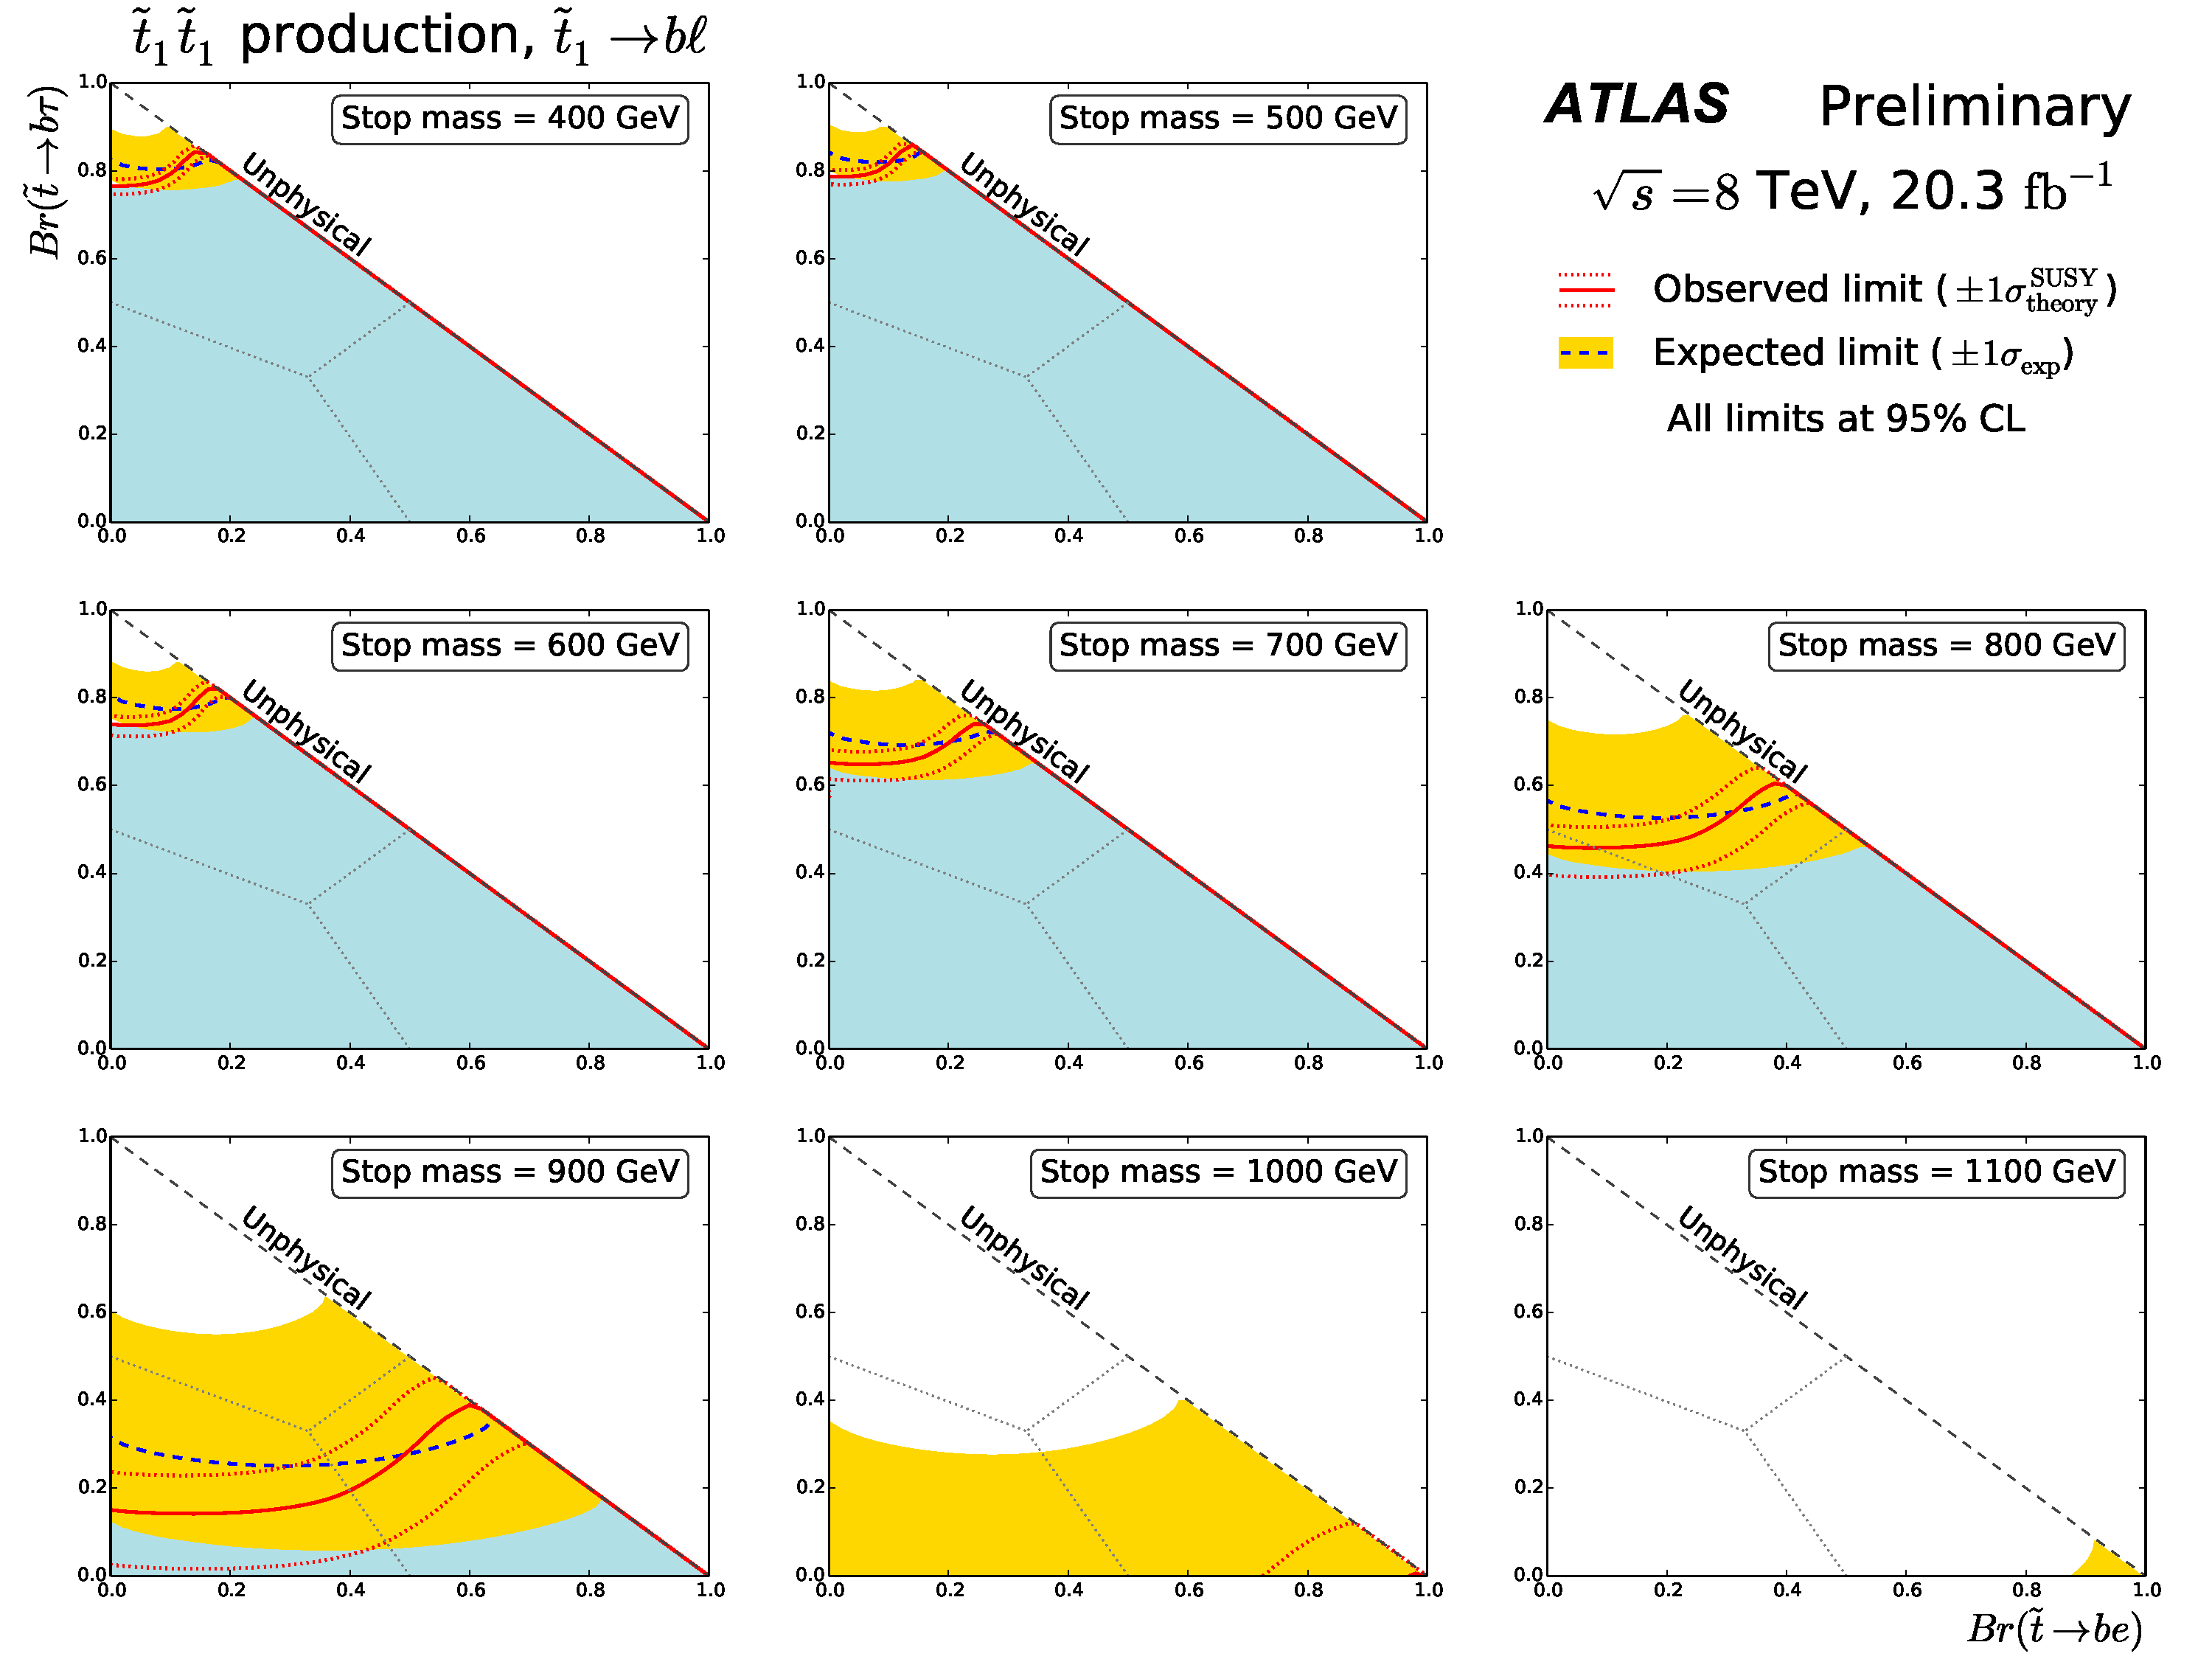
\includegraphics[width=\textwidth]{figs/blstop/limit_contours.pdf}
  \caption{Expected and observed limit on the branching ratios for the stop
    decaying to different lepton flavors shown for different stop mass
    hypotheses between 400~\GeV and 1~\TeV. The shaded area under the solid
    line represents the branching ratios which are excluded at 95\% CL
    for each stop mass.
    The dotted lines represent the uncertainty on the observed mass limit
    obtained by varying the signal model cross section up and down one standard
    deviation from the nominal value. The dashed line shows the
    expected 95\% CL exclusion for each stop mass, and the shaded band shows
    the uncertainty on this expected exclusion limit from statistical
    uncertainty and the sources of systematic uncertainty discussed in
    Section~\ref{sec:systematics}.
  }
  \label{fig:limit_contours}
\end{figure}

\begin{figure}[ht]
  \centering
  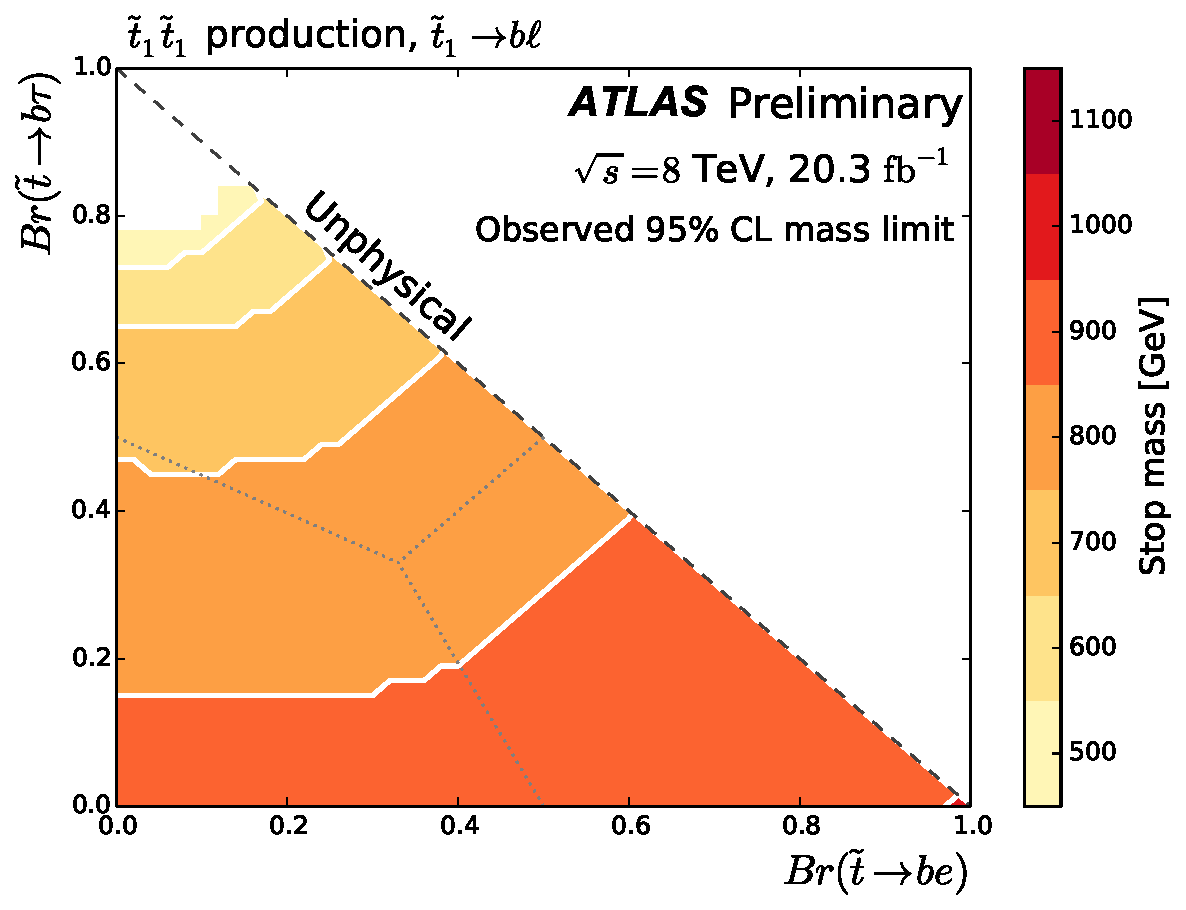
\includegraphics[width=\textwidth]
    {figs/blstop/mass_limit_contours_no_extras_obs.pdf}
  \caption{The observed mass limit on the stop at 95\% CL.
    This limit is obtained using the nominal stop cross section.
    Stop masses between 400~\GeV\ and 1100~\GeV, in steps of 100~\GeV, are
    tested. The mass limit shown corresponds to the highest-mass stop sample
    which was excluded.
    As the branching ratio of $\tilde{t} \rightarrow b\tau$ increases, the
    number of expected events with electrons or muons in the final state
    decreases. Therefore, the limit on the mass decreases.
  }
  \label{fig:mass_limit_obs}
\end{figure}

%% -----------------------------------------------------------------------------
\section{Proposed improvements}
\label{sec:improvements}

